

%%%%%%%%%%%%%%%%%%%%%%%%%%%%%%%%%%%%%%%%%
% University/School Laboratory Report
% LaTeX Template
% Version 3.1 (25/3/14)
%
% This template has been downloaded from:
% http://www.LaTeXTemplates.com
%
% Original author:
% Linux and Unix Users Group at Virginia Tech Wiki 
% (https://vtluug.org/wiki/Example_LaTeX_chem_lab_report)
%
% License:
% CC BY-NC-SA 3.0 (http://creativecommons.org/licenses/by-nc-sa/3.0/)
%
%%%%%%%%%%%%%%%%%%%%%%%%%%%%%%%%%%%%%%%%%

%----------------------------------------------------------------------------------------
%	PACKAGES AND DOCUMENT CONFIGURATIONS
%----------------------------------------------------------------------------------------

\documentclass{article}

\usepackage[version=3]{mhchem} % Package for chemical equation typesetting
\usepackage{siunitx} % Provides the \SI{}{} and \si{} command for typesetting SI units
\usepackage{graphicx} % Required for the inclusion of images
\usepackage{natbib} % Required to change bibliography style to APA
\usepackage{amsmath} % Required for some math elements 
\usepackage{pdfpages} % Required for adding pdf's


\setlength\parindent{0pt} % Removes all indentation from paragraphs

\renewcommand{\labelenumi}{\alph{enumi}.} % Make numbering in the enumerate environment by letter rather than number (e.g. section 6)

%\usepackage{times} % Uncomment to use the Times New Roman font

%----------------------------------------------------------------------------------------
%	DOCUMENT INFORMATION
%----------------------------------------------------------------------------------------

\title{Supplementary material \\  Sub-Saharan Africa sweetpotato virome } % Title

\author{Ricardo I. \textsc{Alcal\'a-Brise\~no}} % Author name

\date{\today} % Date for the report

\begin{document}

\maketitle % Insert the title, author and date

% If you wish to include an abstract, uncomment the lines below
 \begin{abstract}
 Results and supplementary figures of the Sub-Saharan Africa  sweetpotato virome (SSA-SPV).  
 \end{abstract}

%----------------------------------------------------------------------------------------
%	SECTION 1
%----------------------------------------------------------------------------------------

\section{Gravity model}

We evaluate the cropland density of sweetpotato using a cropland connecitvity risk index (Yanru et la., 2020). Implementing a gravity model using a negative exponential distribution using the sweetpotato density of 1degree pixel from the Monfreda and MapSpam databases (REFs). 


\begin{figure}[h!]
\begin{center}
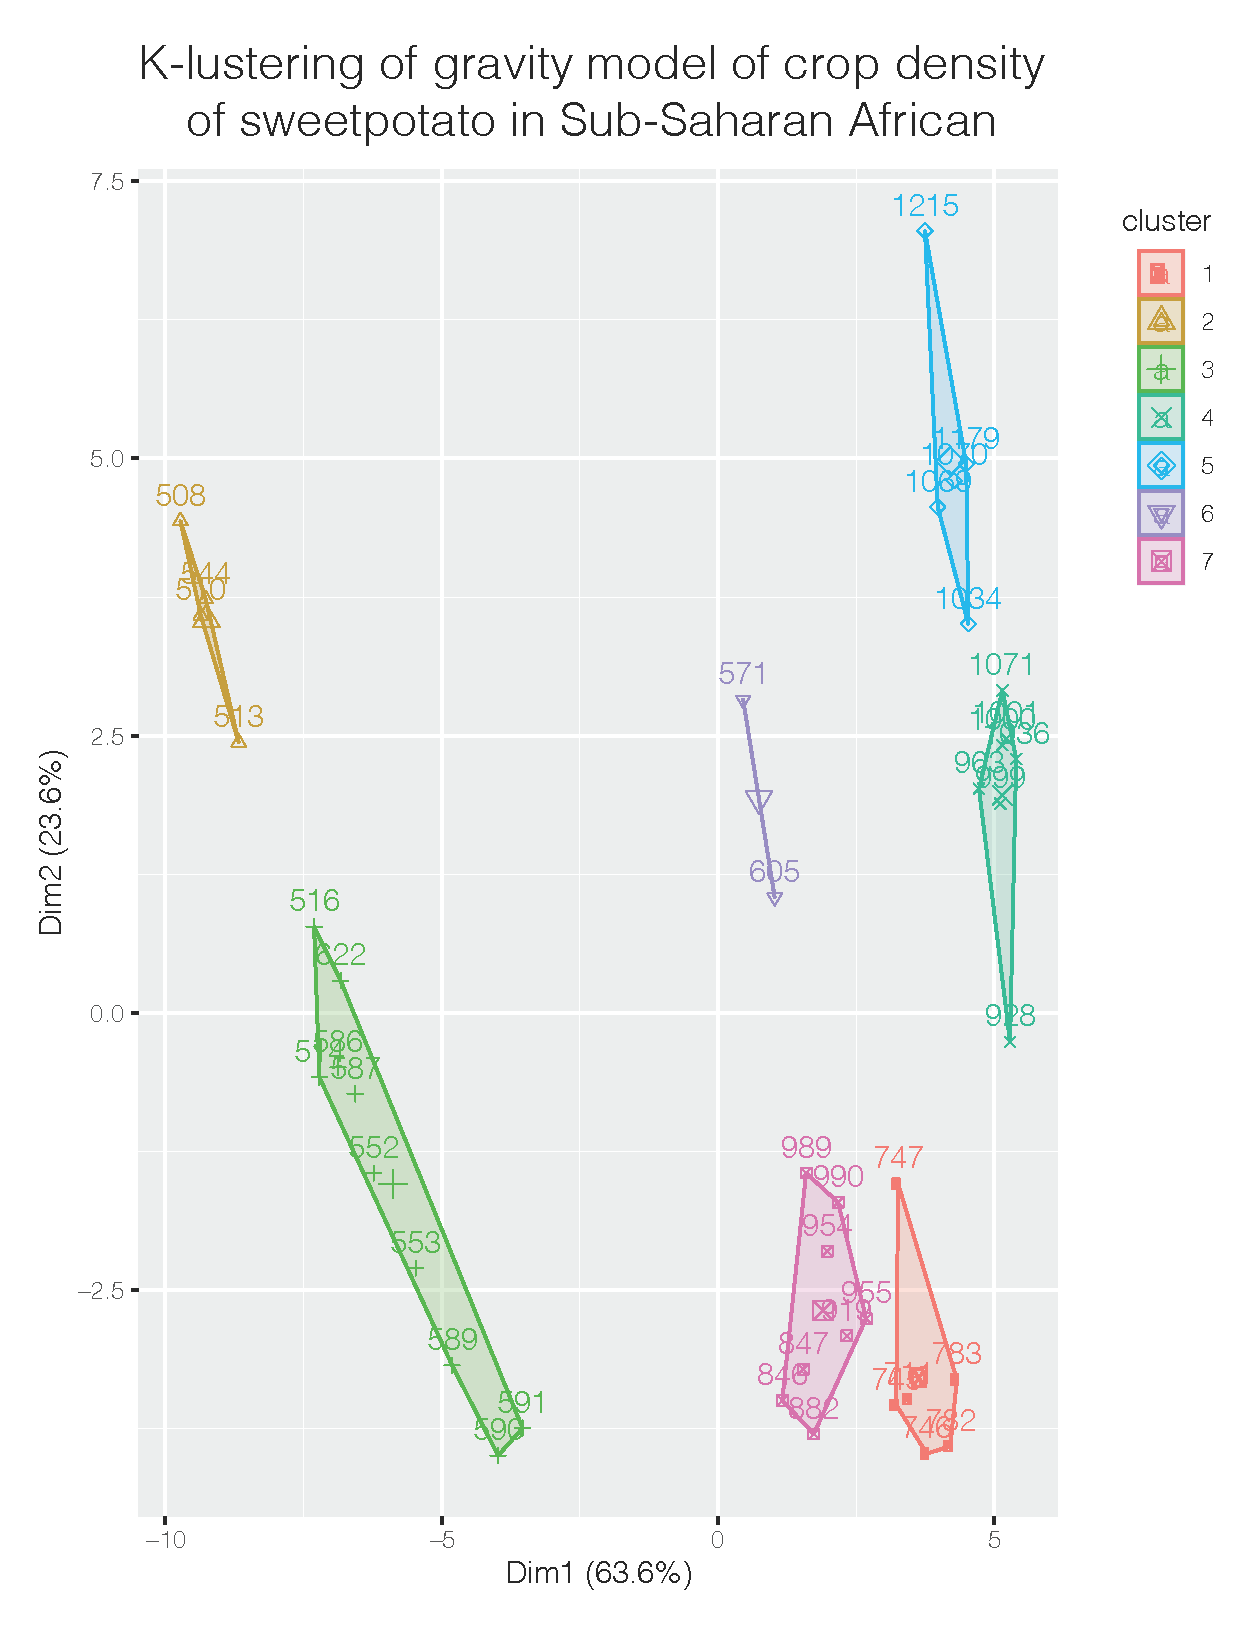
\includegraphics[width=0.45\textwidth]{../images/SSA-SPV-kcluster-1gamma-2_deg_1e-06_gap_statsMC1000} % Include the image placeholder.png
\caption{Gravity model Sub-Saharan Africa sweetpotato virome.}
\end{center}
\end{figure}

\begin{center}\ce{2 Mg + O2 -> 2 MgO}\end{center}

% If you have more than one objective, uncomment the below:
%\begin{description}
%\item[First Objective] \hfill \\
%Objective 1 text
%\item[Second Objective] \hfill \\
%Objective 2 text
%\end{description}

\subsection{Regions}
\label{Sweetpotato regions}
Seven regions of sweetpotato were identified with a gravity model (table 1).

\begin{table}[h!]
\begin{tabular}{lclc}
\hline \hline
K-cluster  & Regions      	& Countries                      			& Samples \\ \hline
Region 1  & East           	& Tanzania, Uganda                			& 228        \\
Region 2  & Near West      & Ghana, Benin and Nigeria      		& 36          \\
Region 3  & Southwest      & Angola                         				& 171        \\
Region 4  & East group 1   & Mozambique, Zimbabwe           		& 262         \\
Region 5  & East group 2   & Mozambique, Tanzania, Zimbabwe 	& 151         \\
Region 6  & East group 3   & Rwanda, Tanzania, Uganda       		& 261         \\
Region 7  & Far East       	& Ethiopia                      	 			& 171         \\ 
Total     	  &                	&                                				& 1286       \\  
\hline \hline
\end{tabular}
\end{table}

 
%----------------------------------------------------------------------------------------
%	SECTION 2
%----------------------------------------------------------------------------------------

\section{Regions}



\subsection{Region 1}

Region 1 corresponding to East Africa (Tanzania and Uganda) of 228 samples collected. We identified 98 viruses species, in \_\_\_\_\_\_\_ genera, and \_\_\_\_\_\_ families.  A barplot representing the frequency distribution and relative abundance of SSA-SPV region 1 (Fig. 2)

\begin{figure}[h!]
\begin{center}
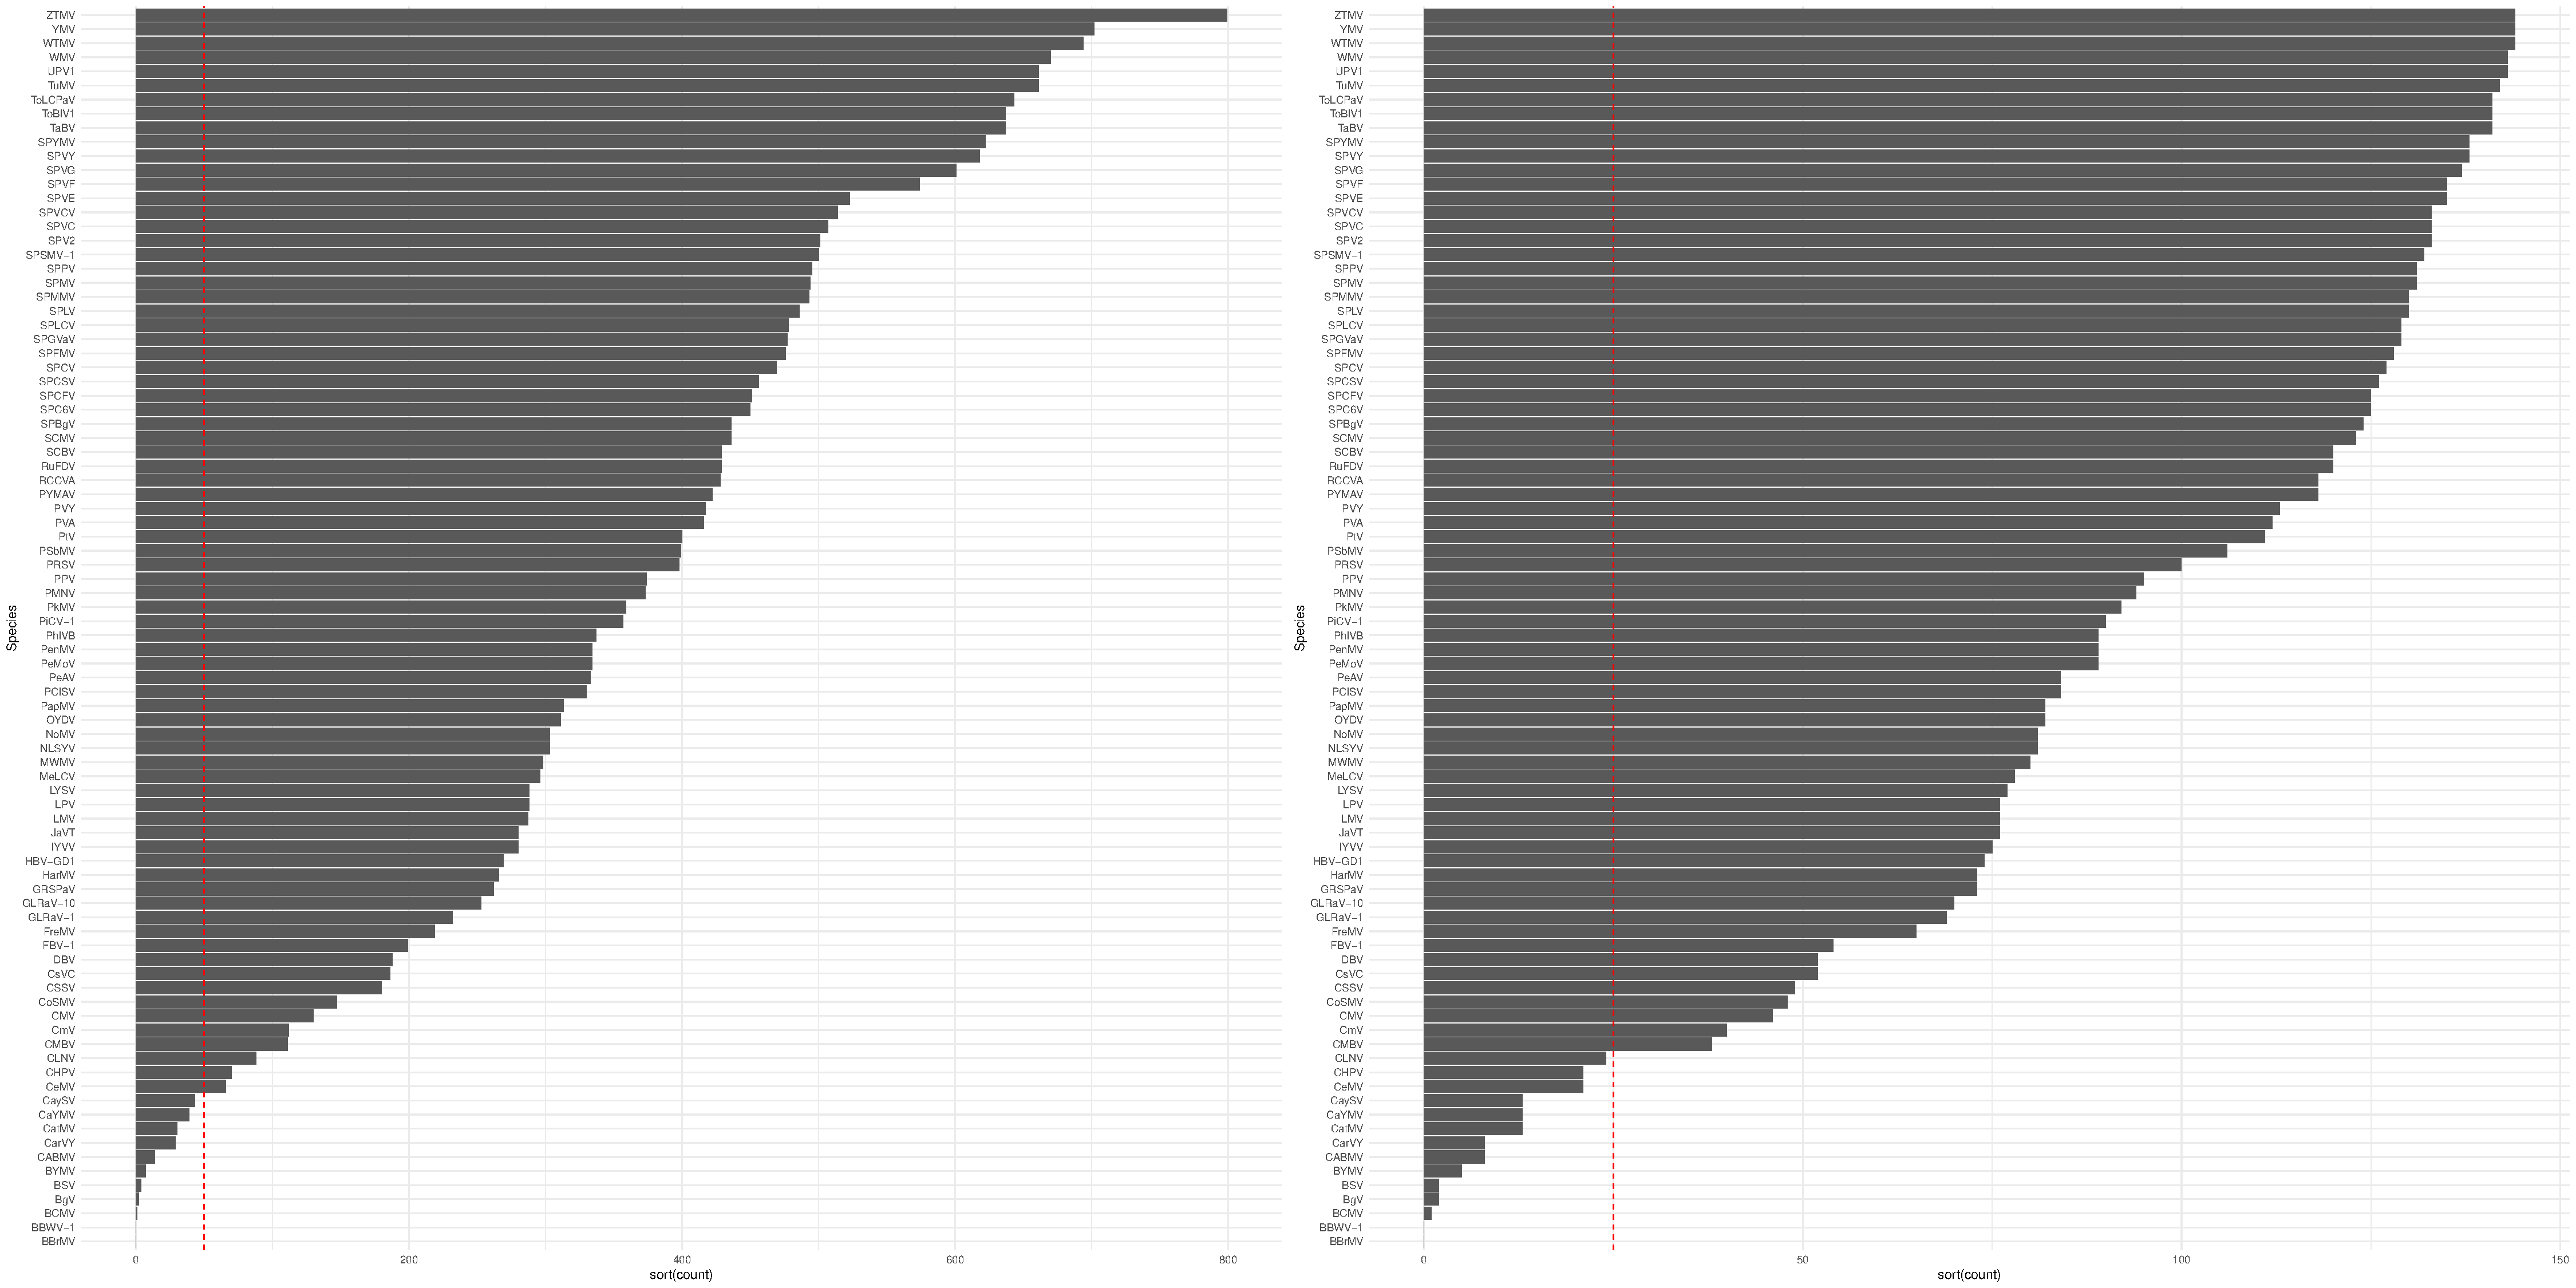
\includegraphics[width=0.95\textwidth]{../results/k-cluster1/1-kcluster_incidence_w+bFeb28.pdf
} % Include the image placeholder.png
\caption{Incidence distribution Sub-Saharan Africa sweetpotato virome region 1.}
\end{center}
\end{figure}


\begin{figure}[h!]
\begin{center}
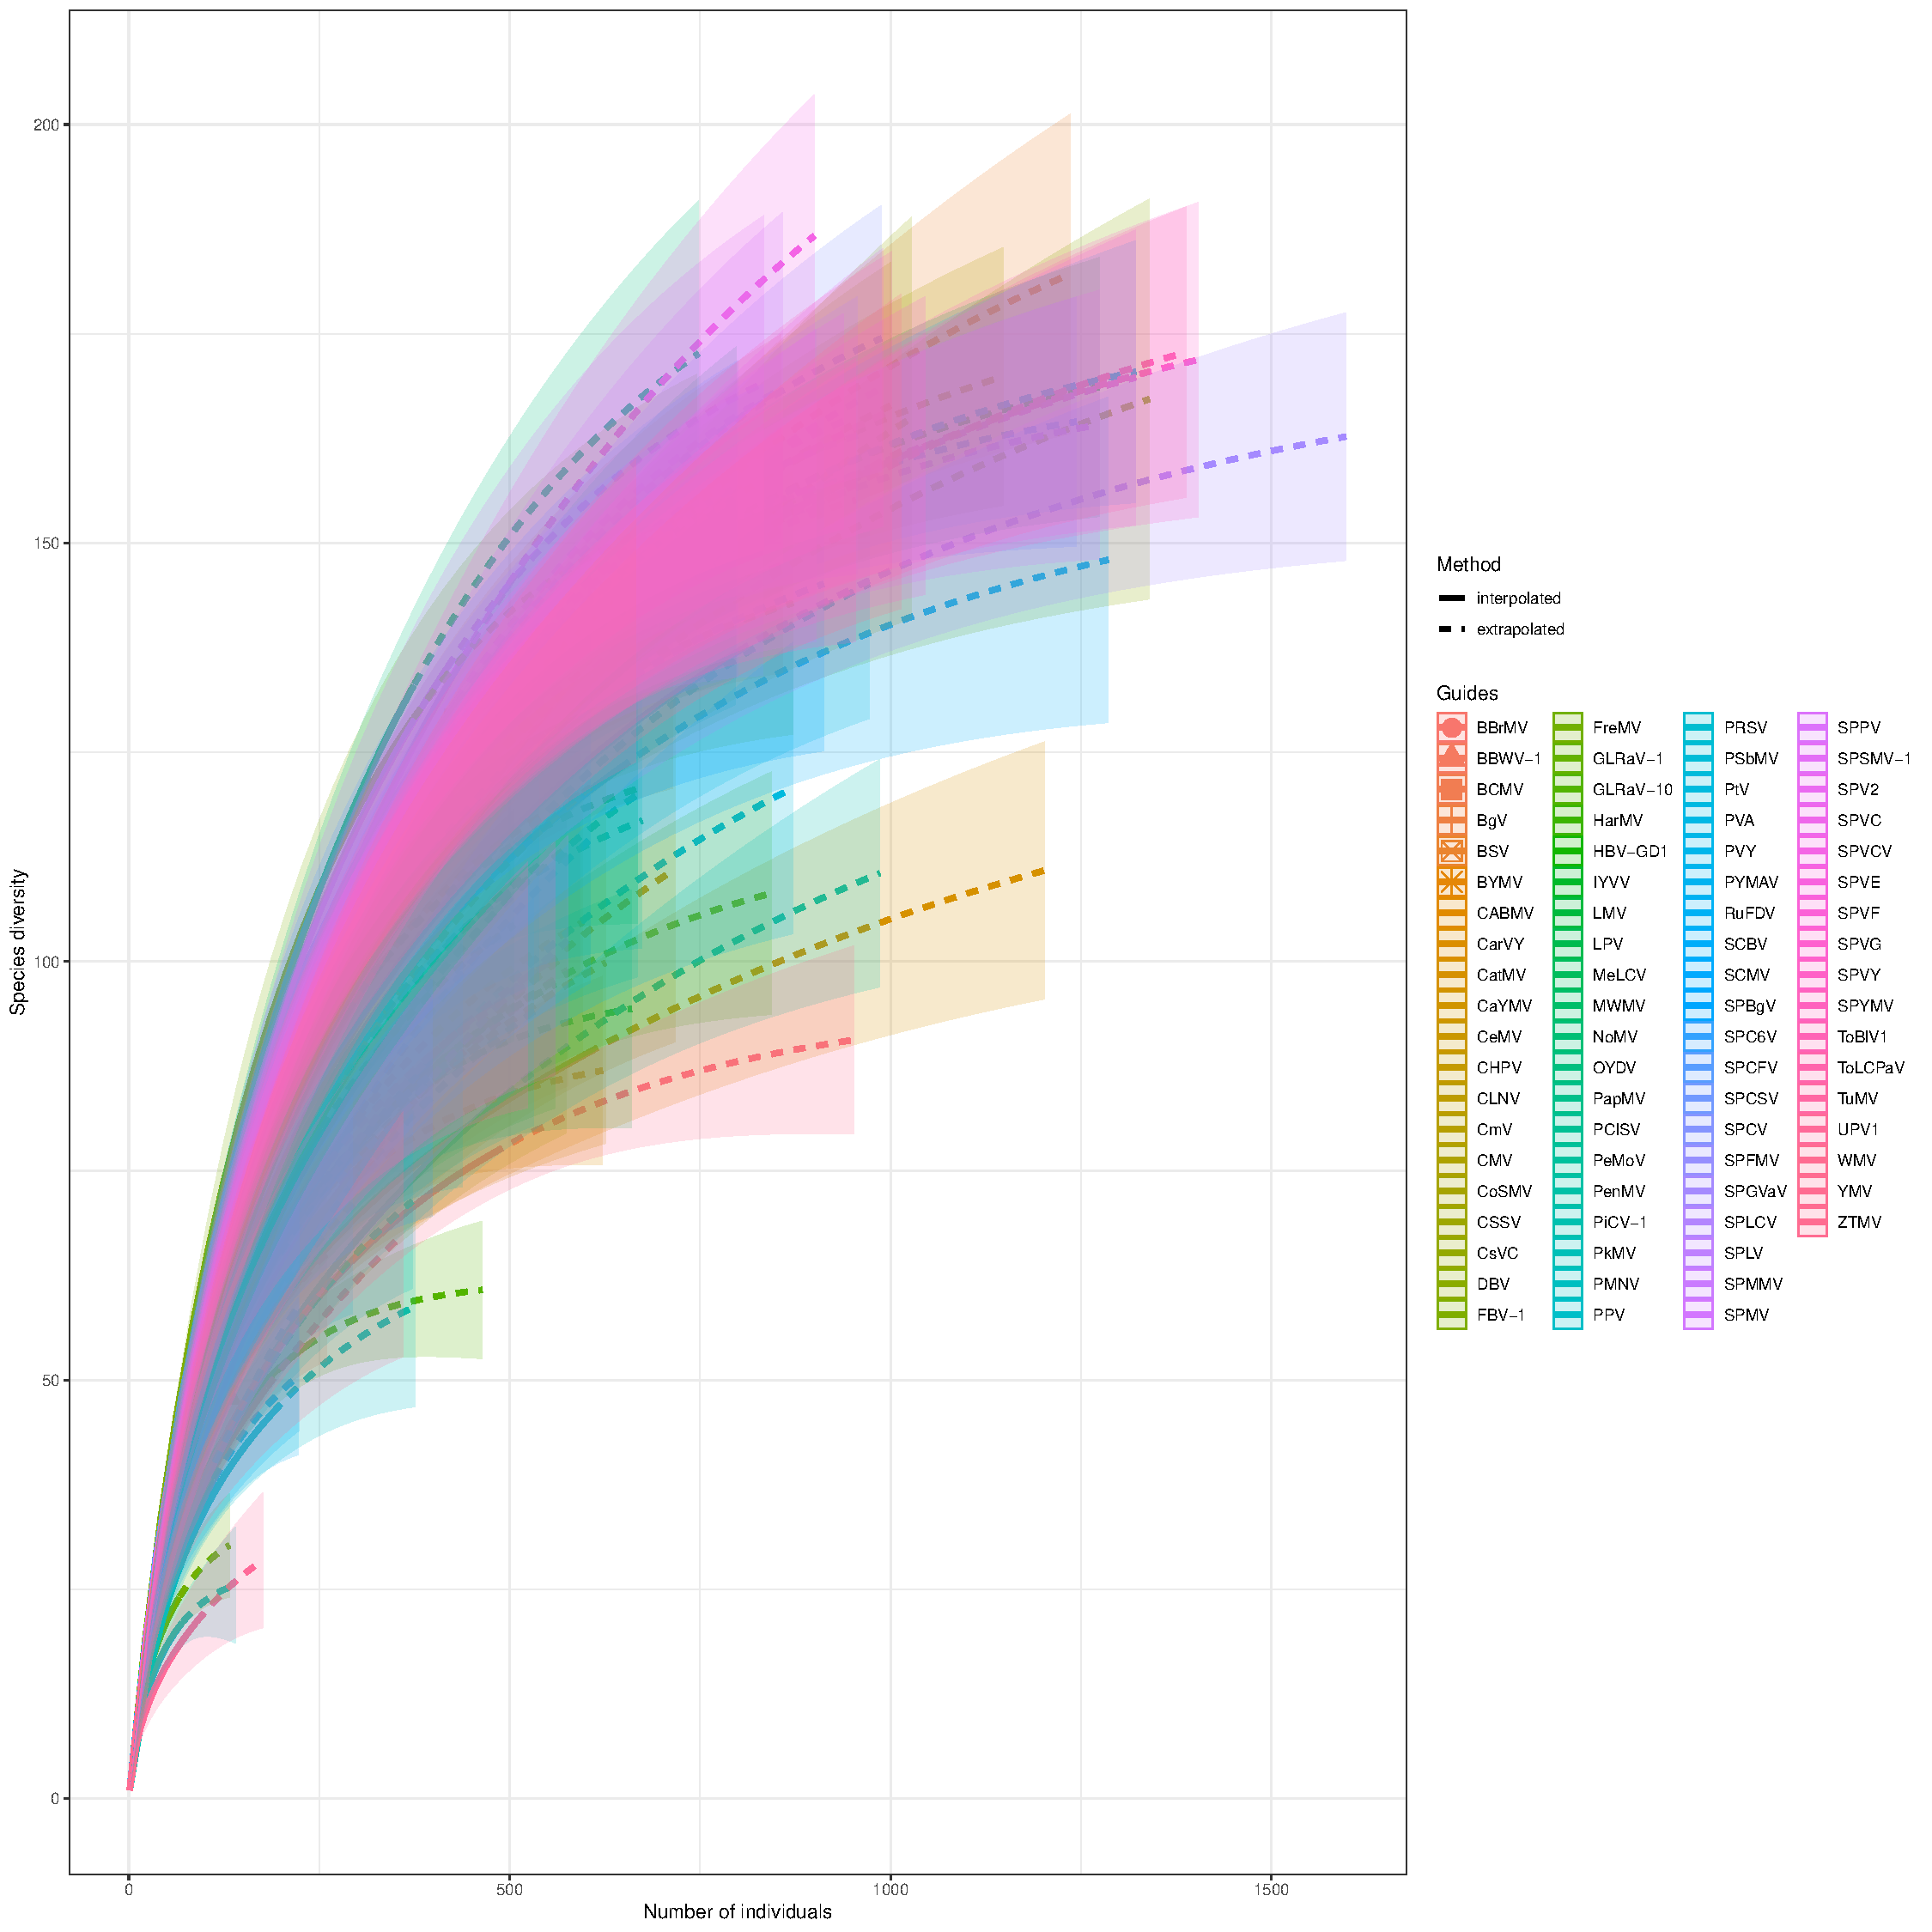
\includegraphics[width=0.75\textwidth]{../results/k-cluster1/1-kcluster_rarefaction-iNEXT_Feb28.pdf
} % Include the image placeholder.png
\caption{Rarefaction of Sub-Saharan Africa sweetpotato virome region 1.}
\end{center}
\end{figure}


\begin{figure}[h!]
\begin{center}
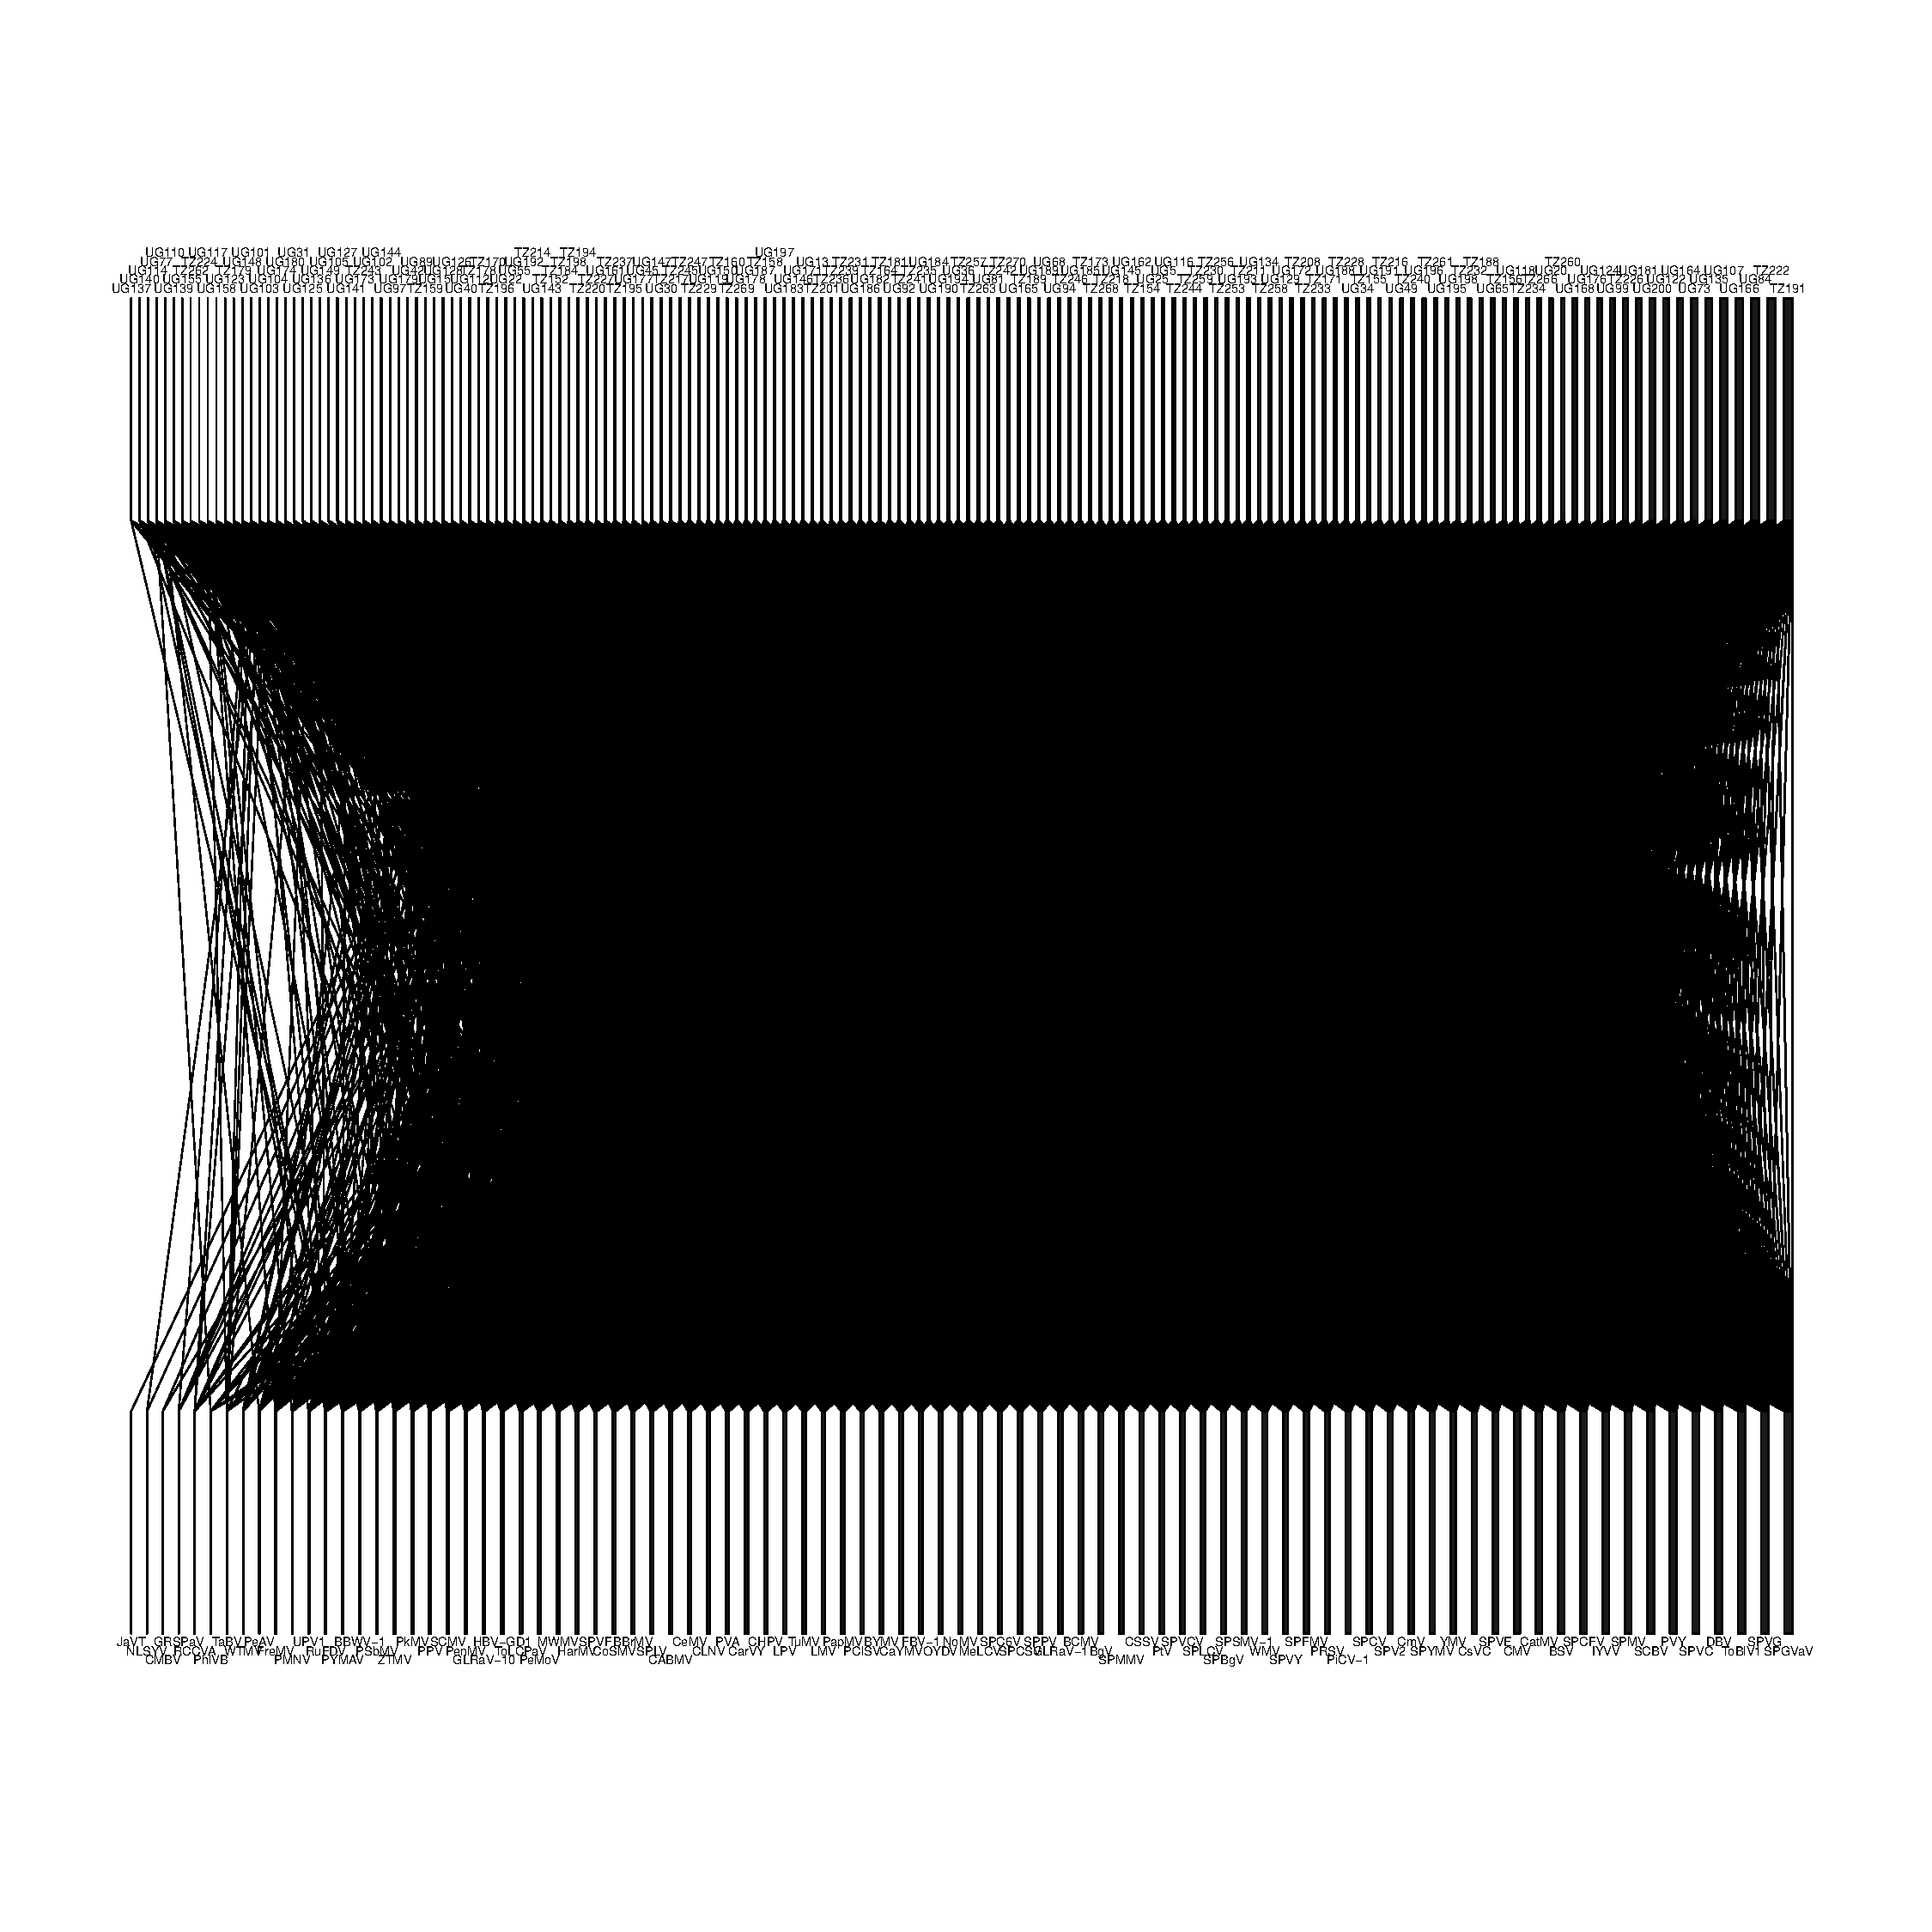
\includegraphics[width=0.75\textwidth]{../results/k-cluster1/1-kcluster_bipartitenetwork_Feb28.pdf
} % Include the image placeholder.png
\caption{Bipartite network Sub-Saharan Africa sweetpotato virome region 1.}
\end{center}
\end{figure}



\begin{figure}[h!]
\begin{center}
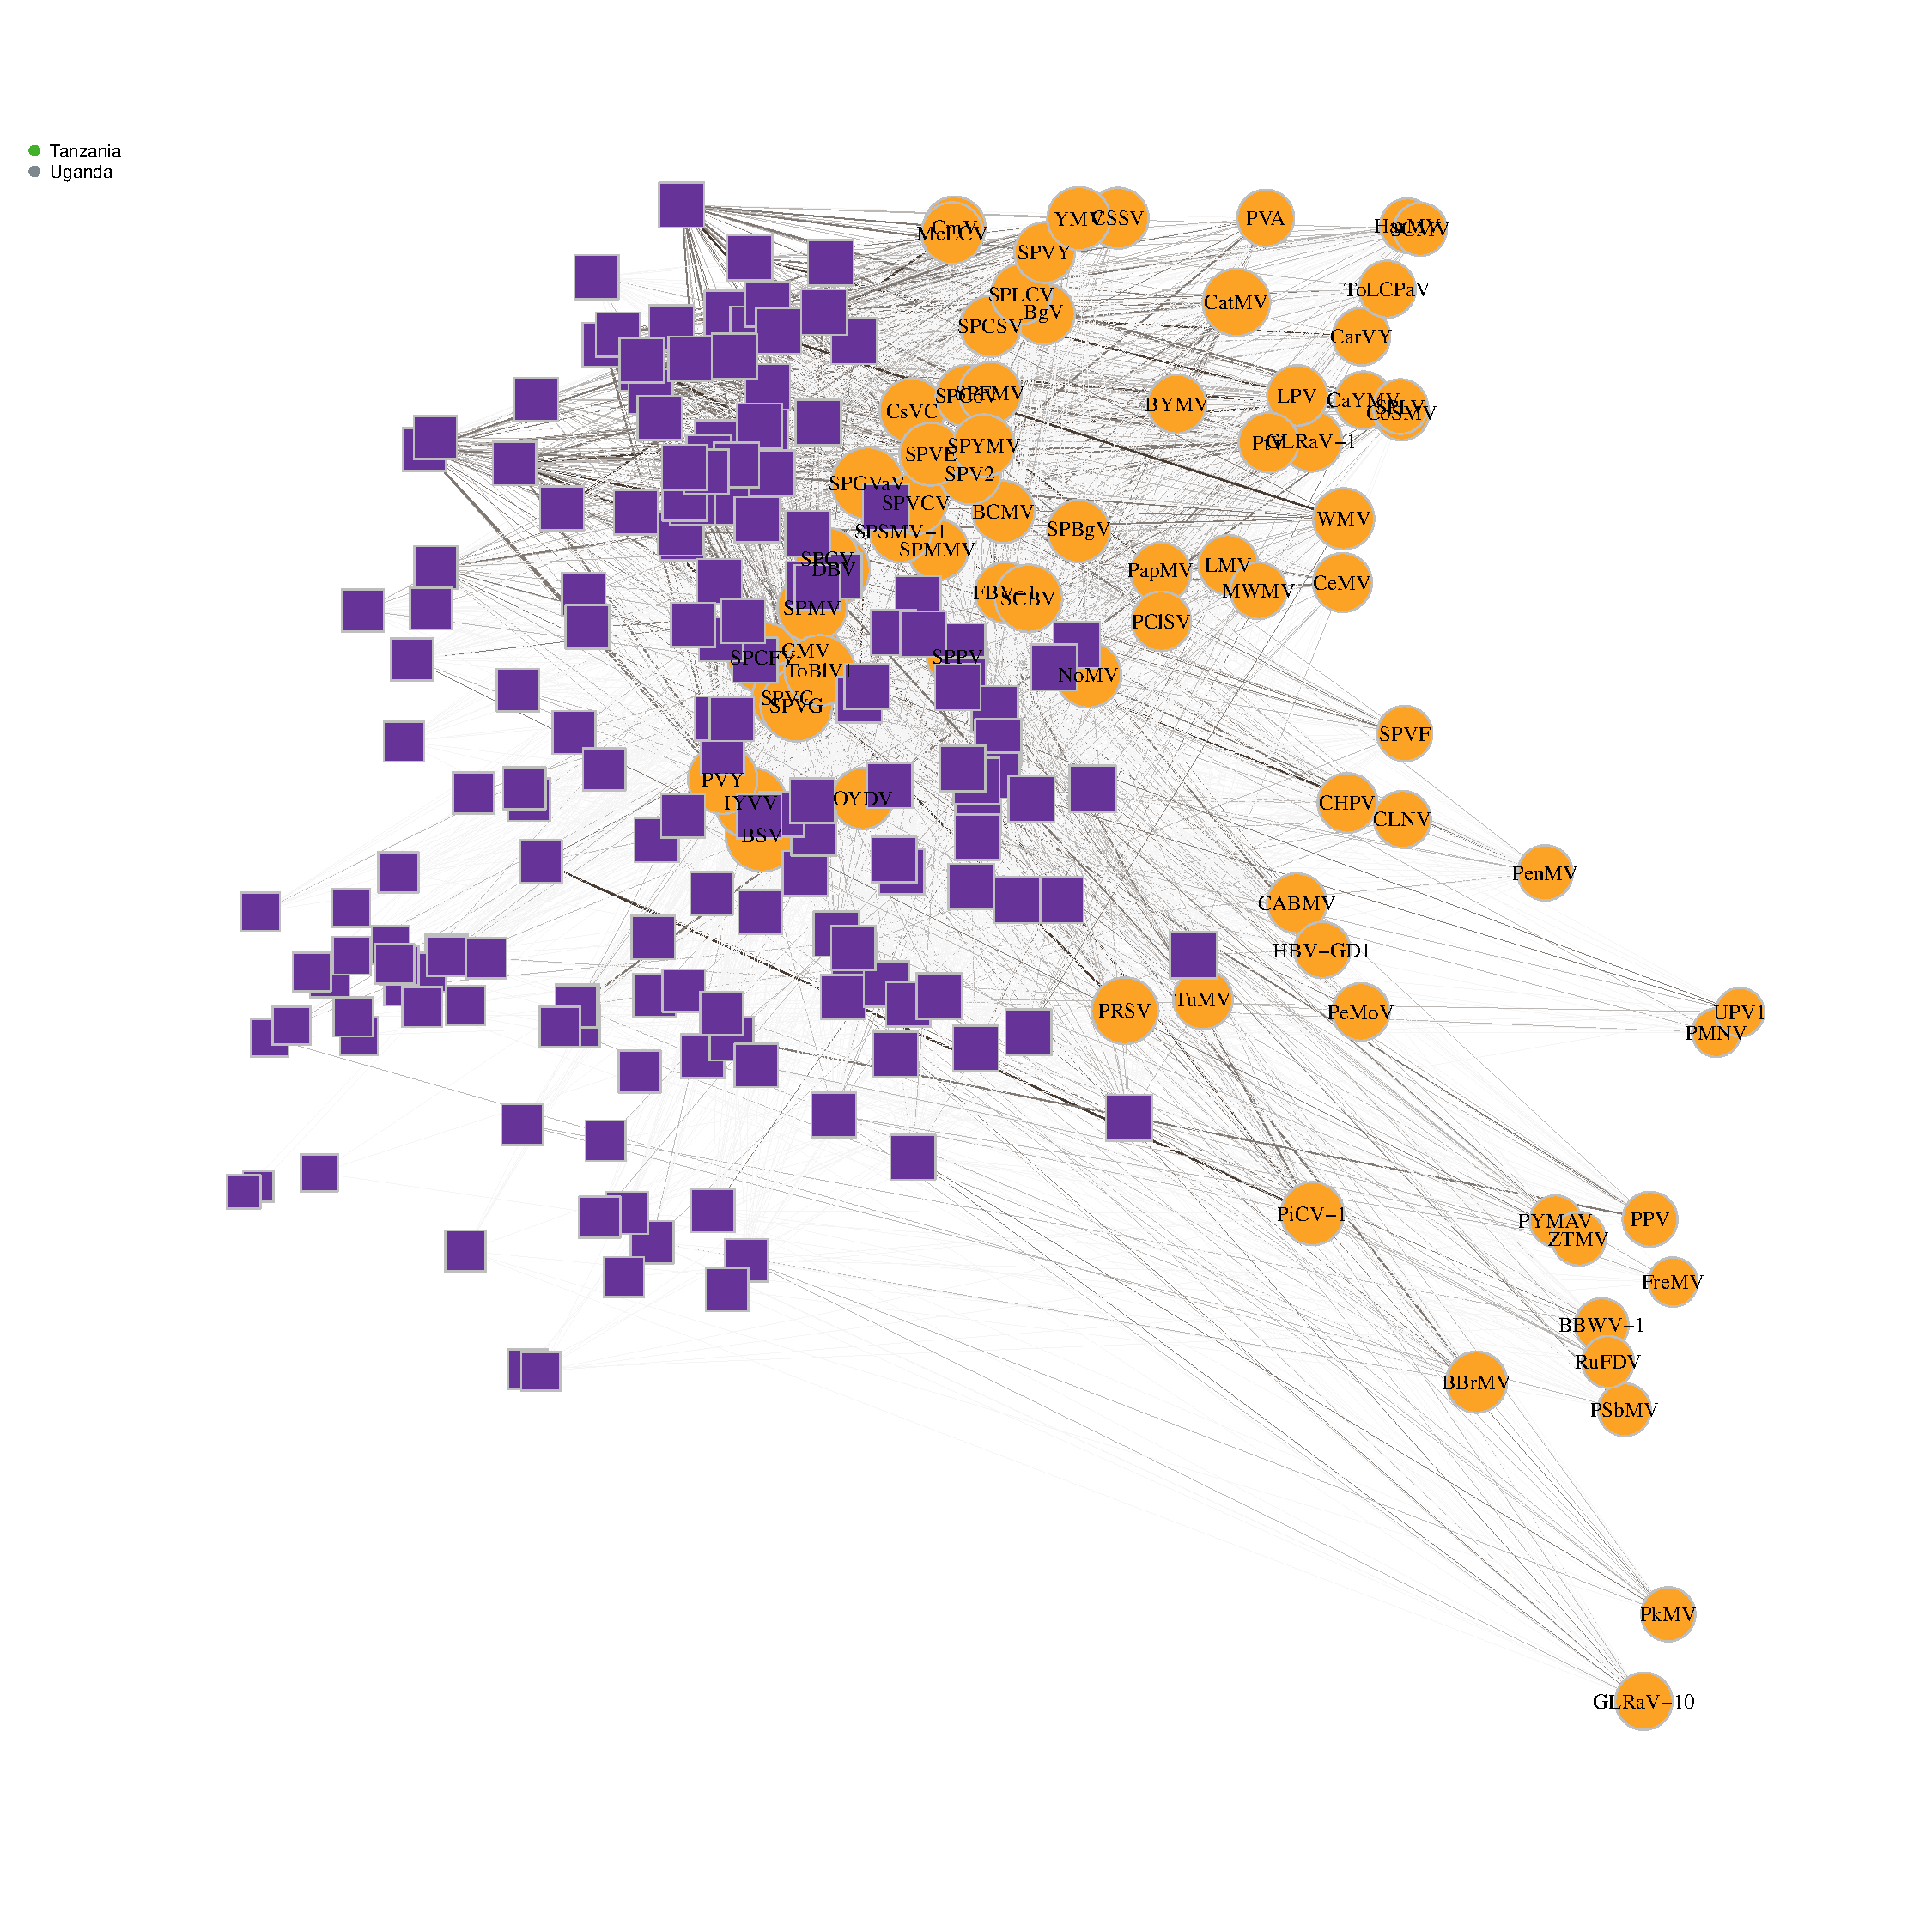
\includegraphics[width=0.85\textwidth]{../results/k-cluster1/1-kcluster_bipartitenetwork-kk_Feb28.pdf
} % Include the image placeholder.png
\caption{Bipartite network Sub-Saharan Africa sweetpotato virome region 1, Kimura-Kawai layout}
\end{center}
\end{figure}


\subsection{Region 2}
\begin{figure}[h!]
\begin{center}
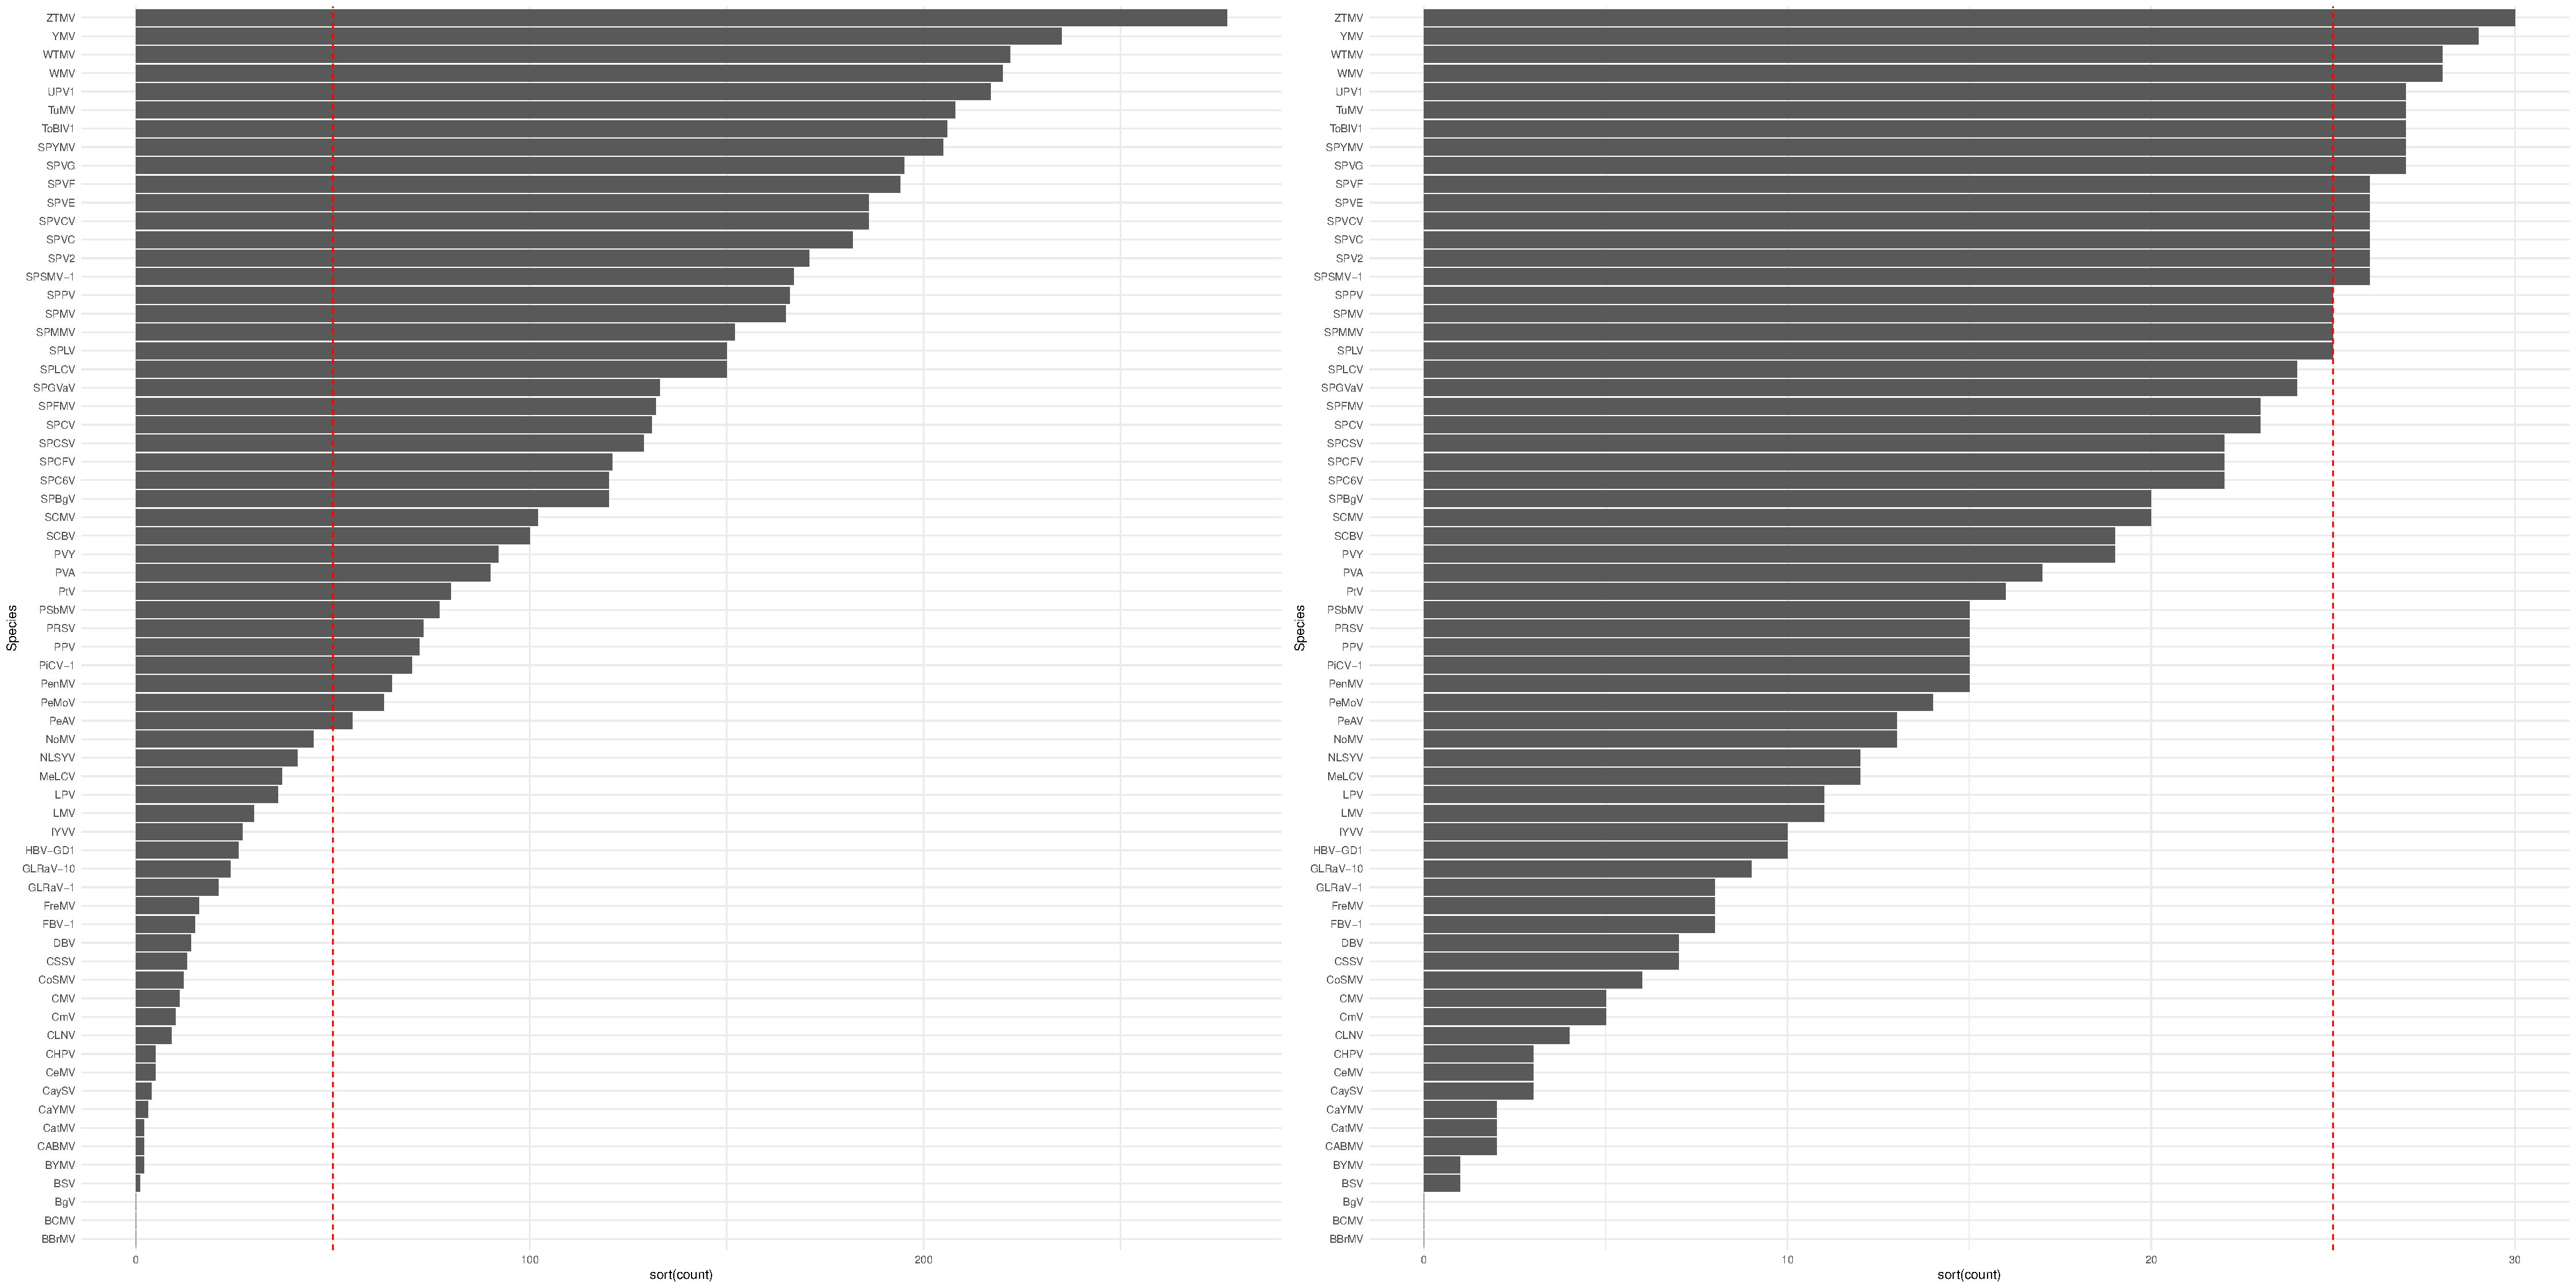
\includegraphics[width=0.95\textwidth]{../results/k-cluster2/2-kcluster_incidence_w+bFeb28.pdf
} % Include the image placeholder.png
\caption{Incidence distribution Sub-Saharan Africa sweetpotato virome region 1.}
\end{center}
\end{figure}


\begin{figure}[h!]
\begin{center}
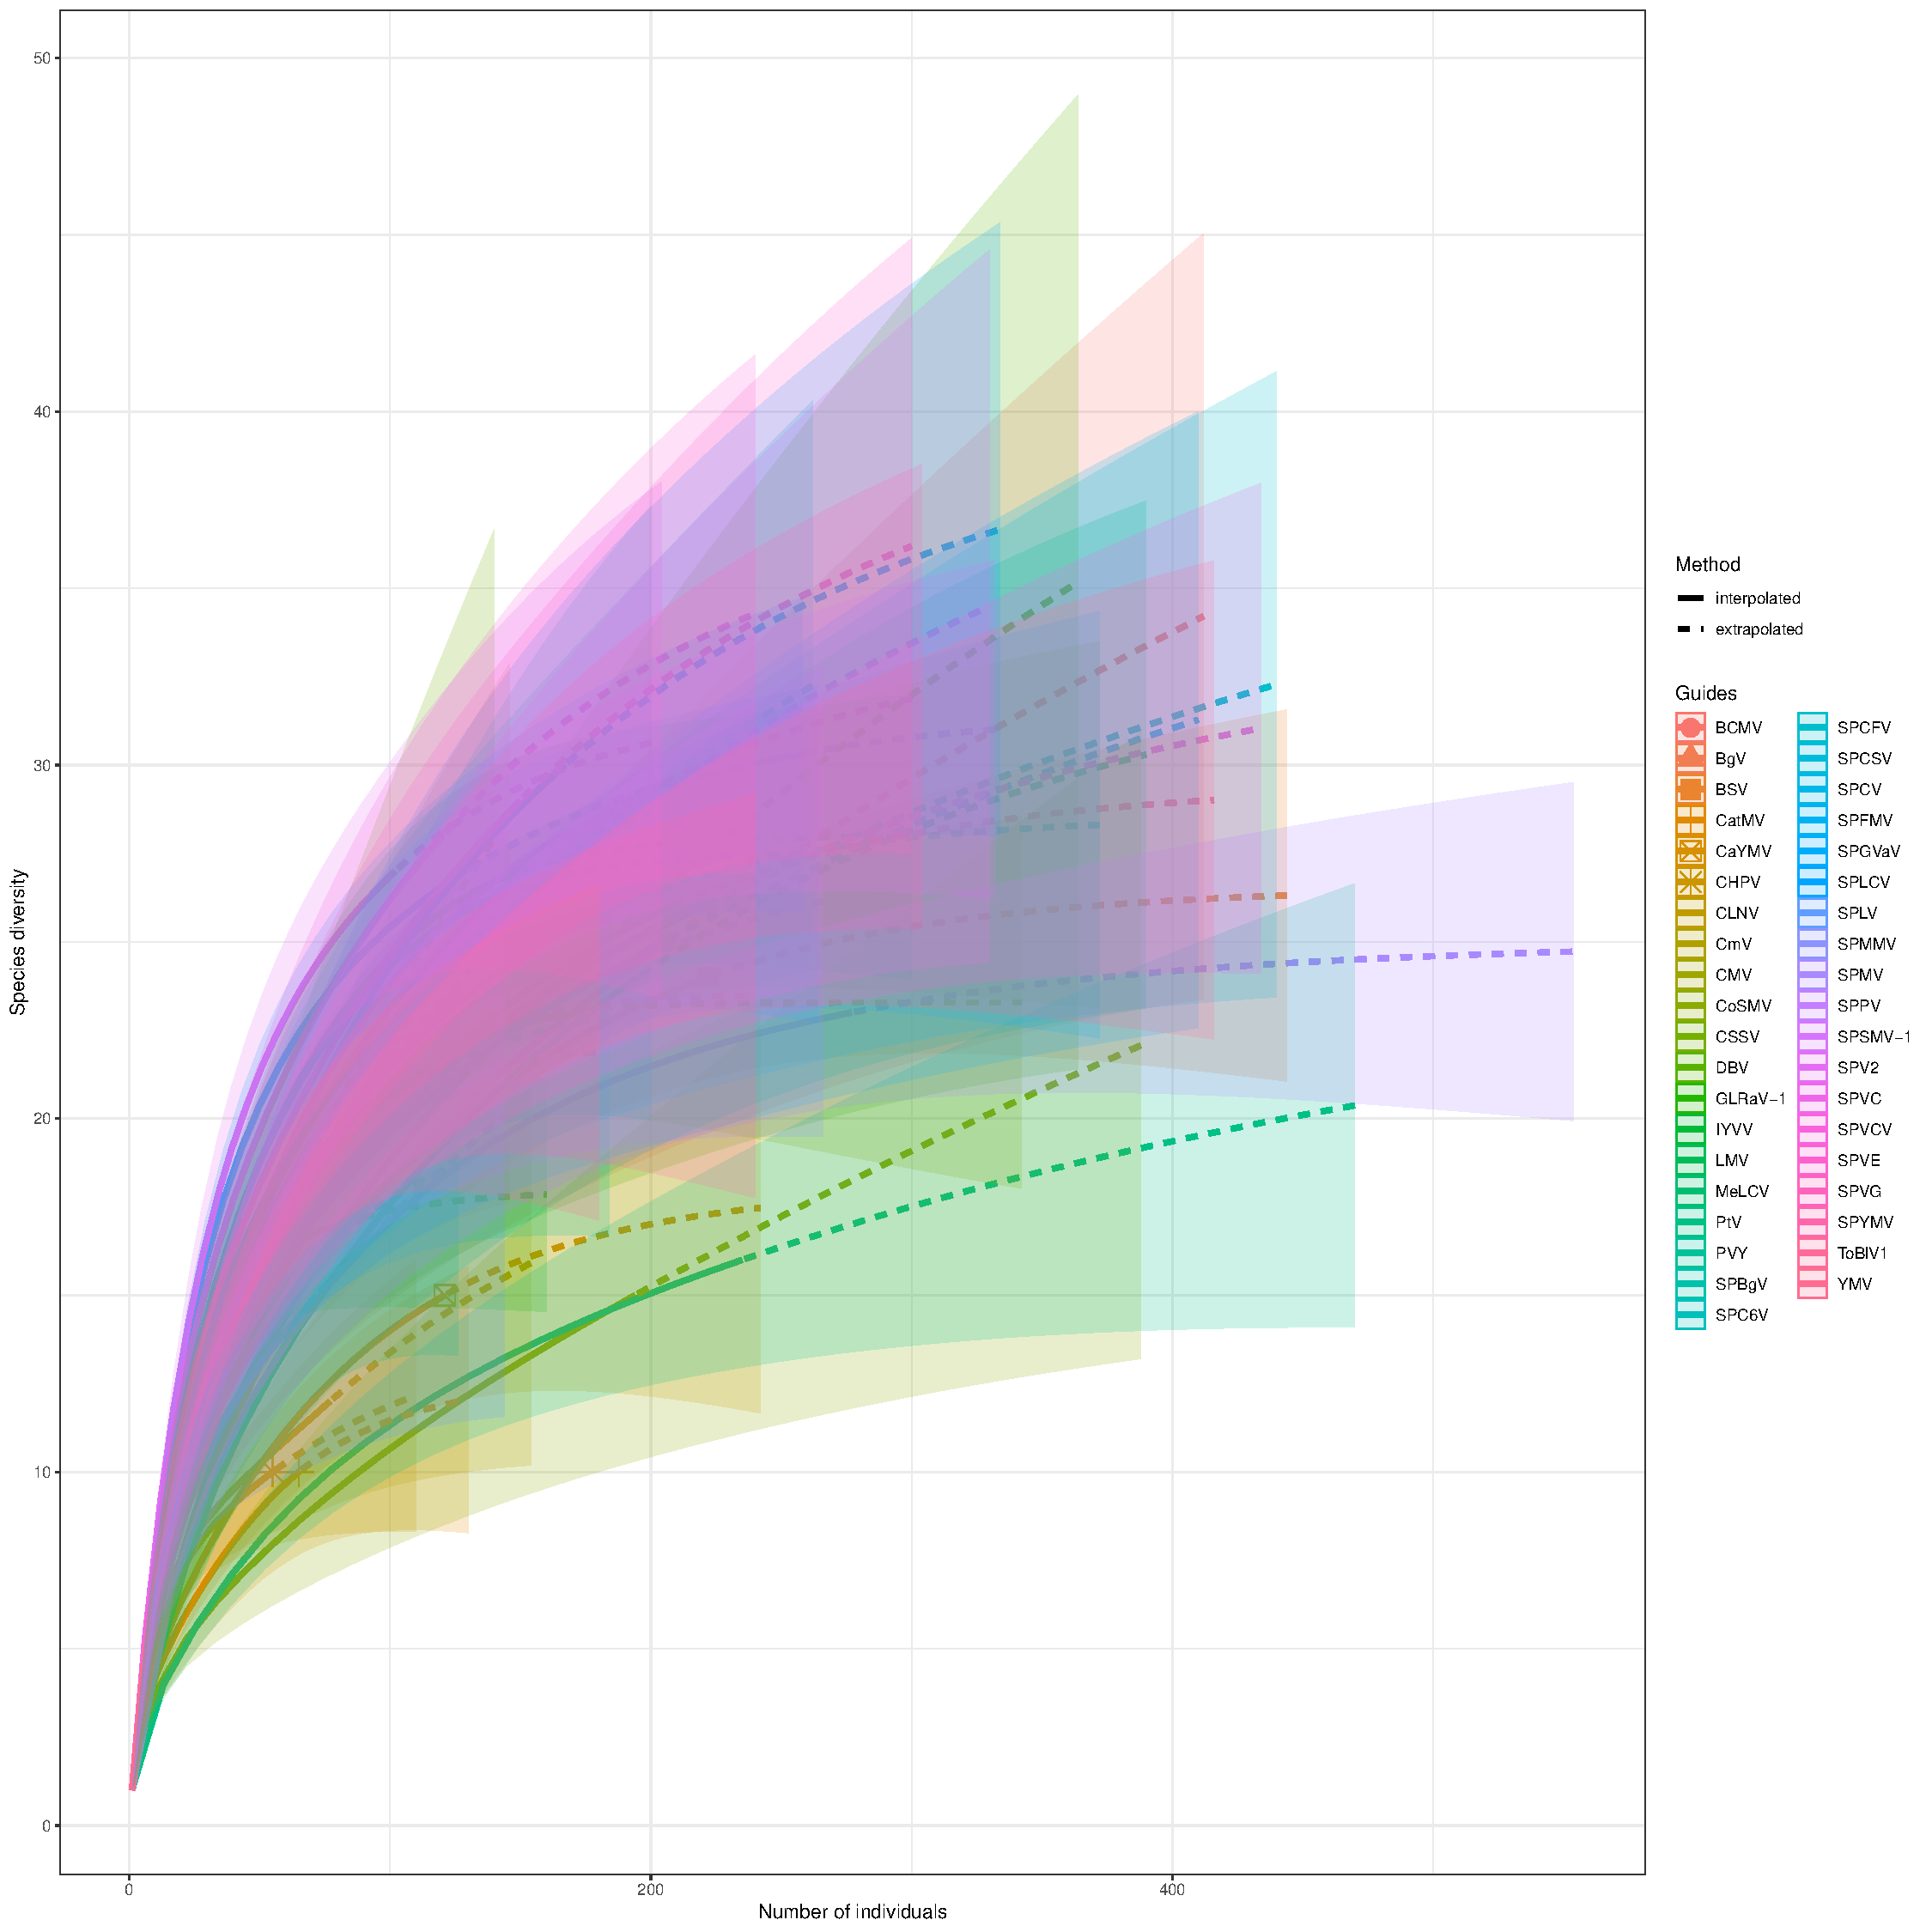
\includegraphics[width=0.75\textwidth]{../results/k-cluster2/2-kcluster_rarefaction-iNEXT_Feb28.pdf
} % Include the image placeholder.png
\caption{Rarefaction of Sub-Saharan Africa sweetpotato virome region 1.}
\end{center}
\end{figure}


\begin{figure}[h!]
\begin{center}
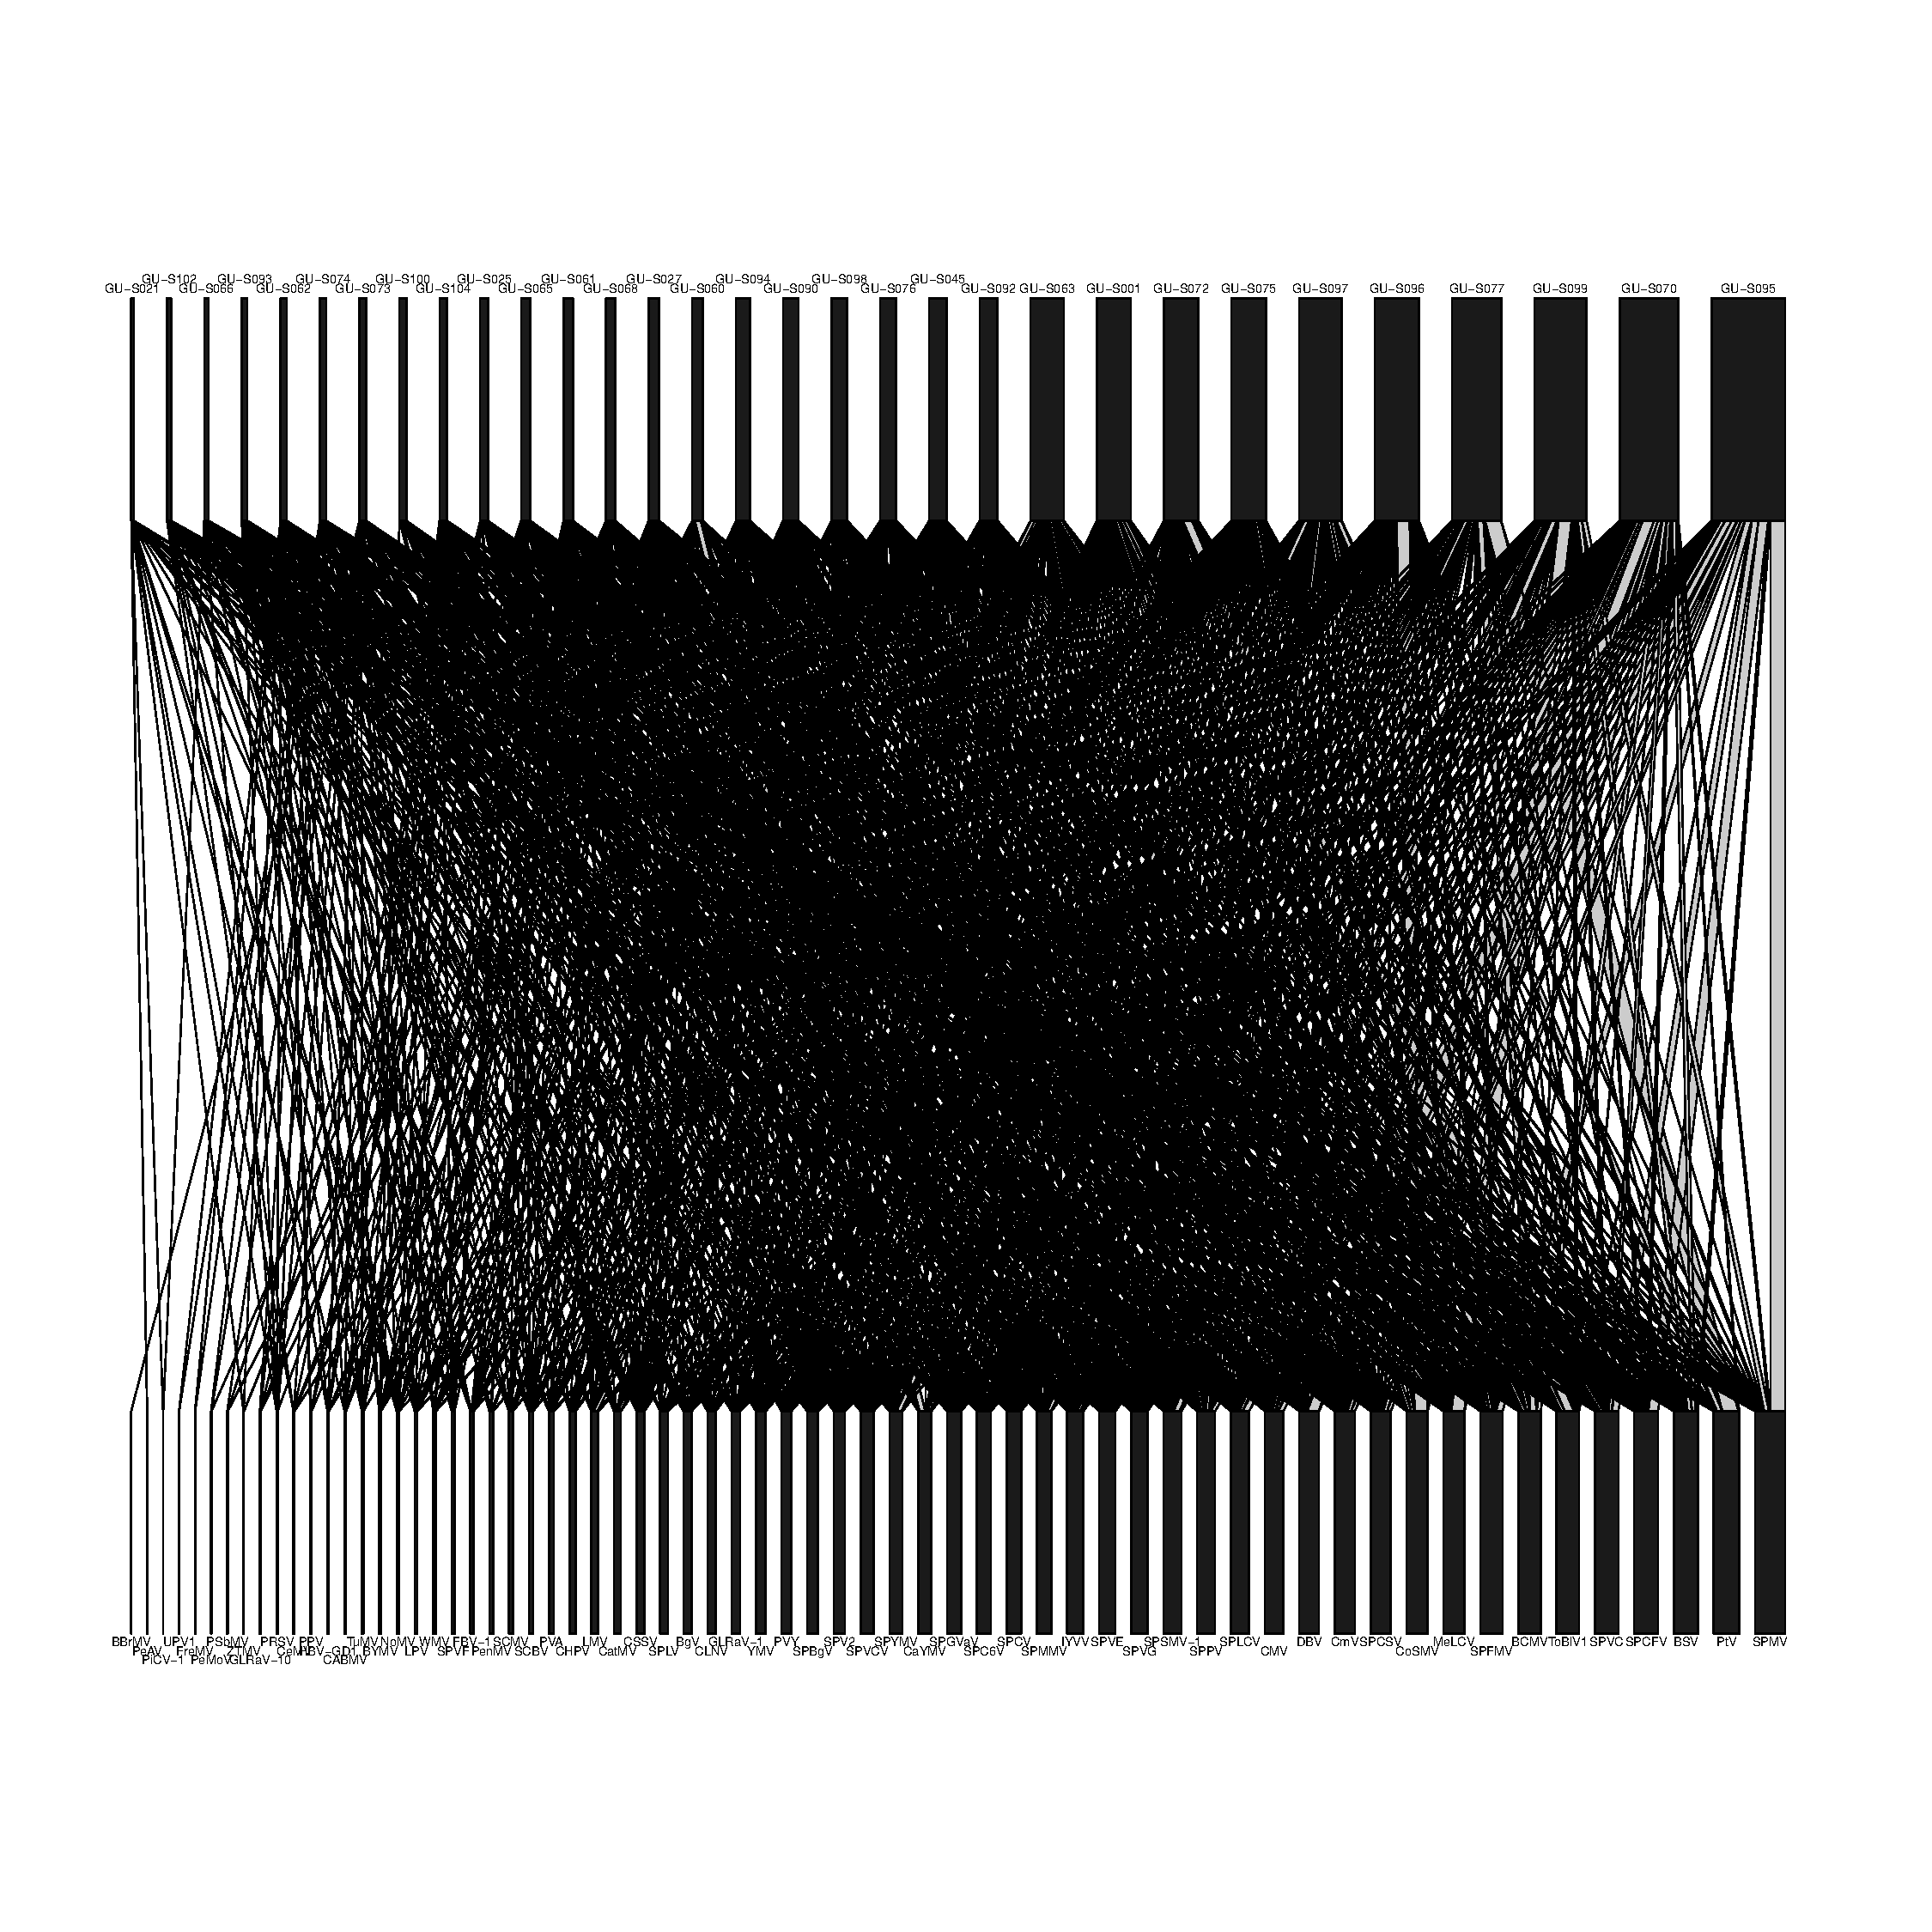
\includegraphics[width=0.75\textwidth]{../results/k-cluster2/2-kcluster_bipartitenetwork_Feb28.pdf
} % Include the image placeholder.png
\caption{Bipartite network Sub-Saharan Africa sweetpotato virome region 1.}
\end{center}
\end{figure}



\begin{figure}[h!]
\begin{center}
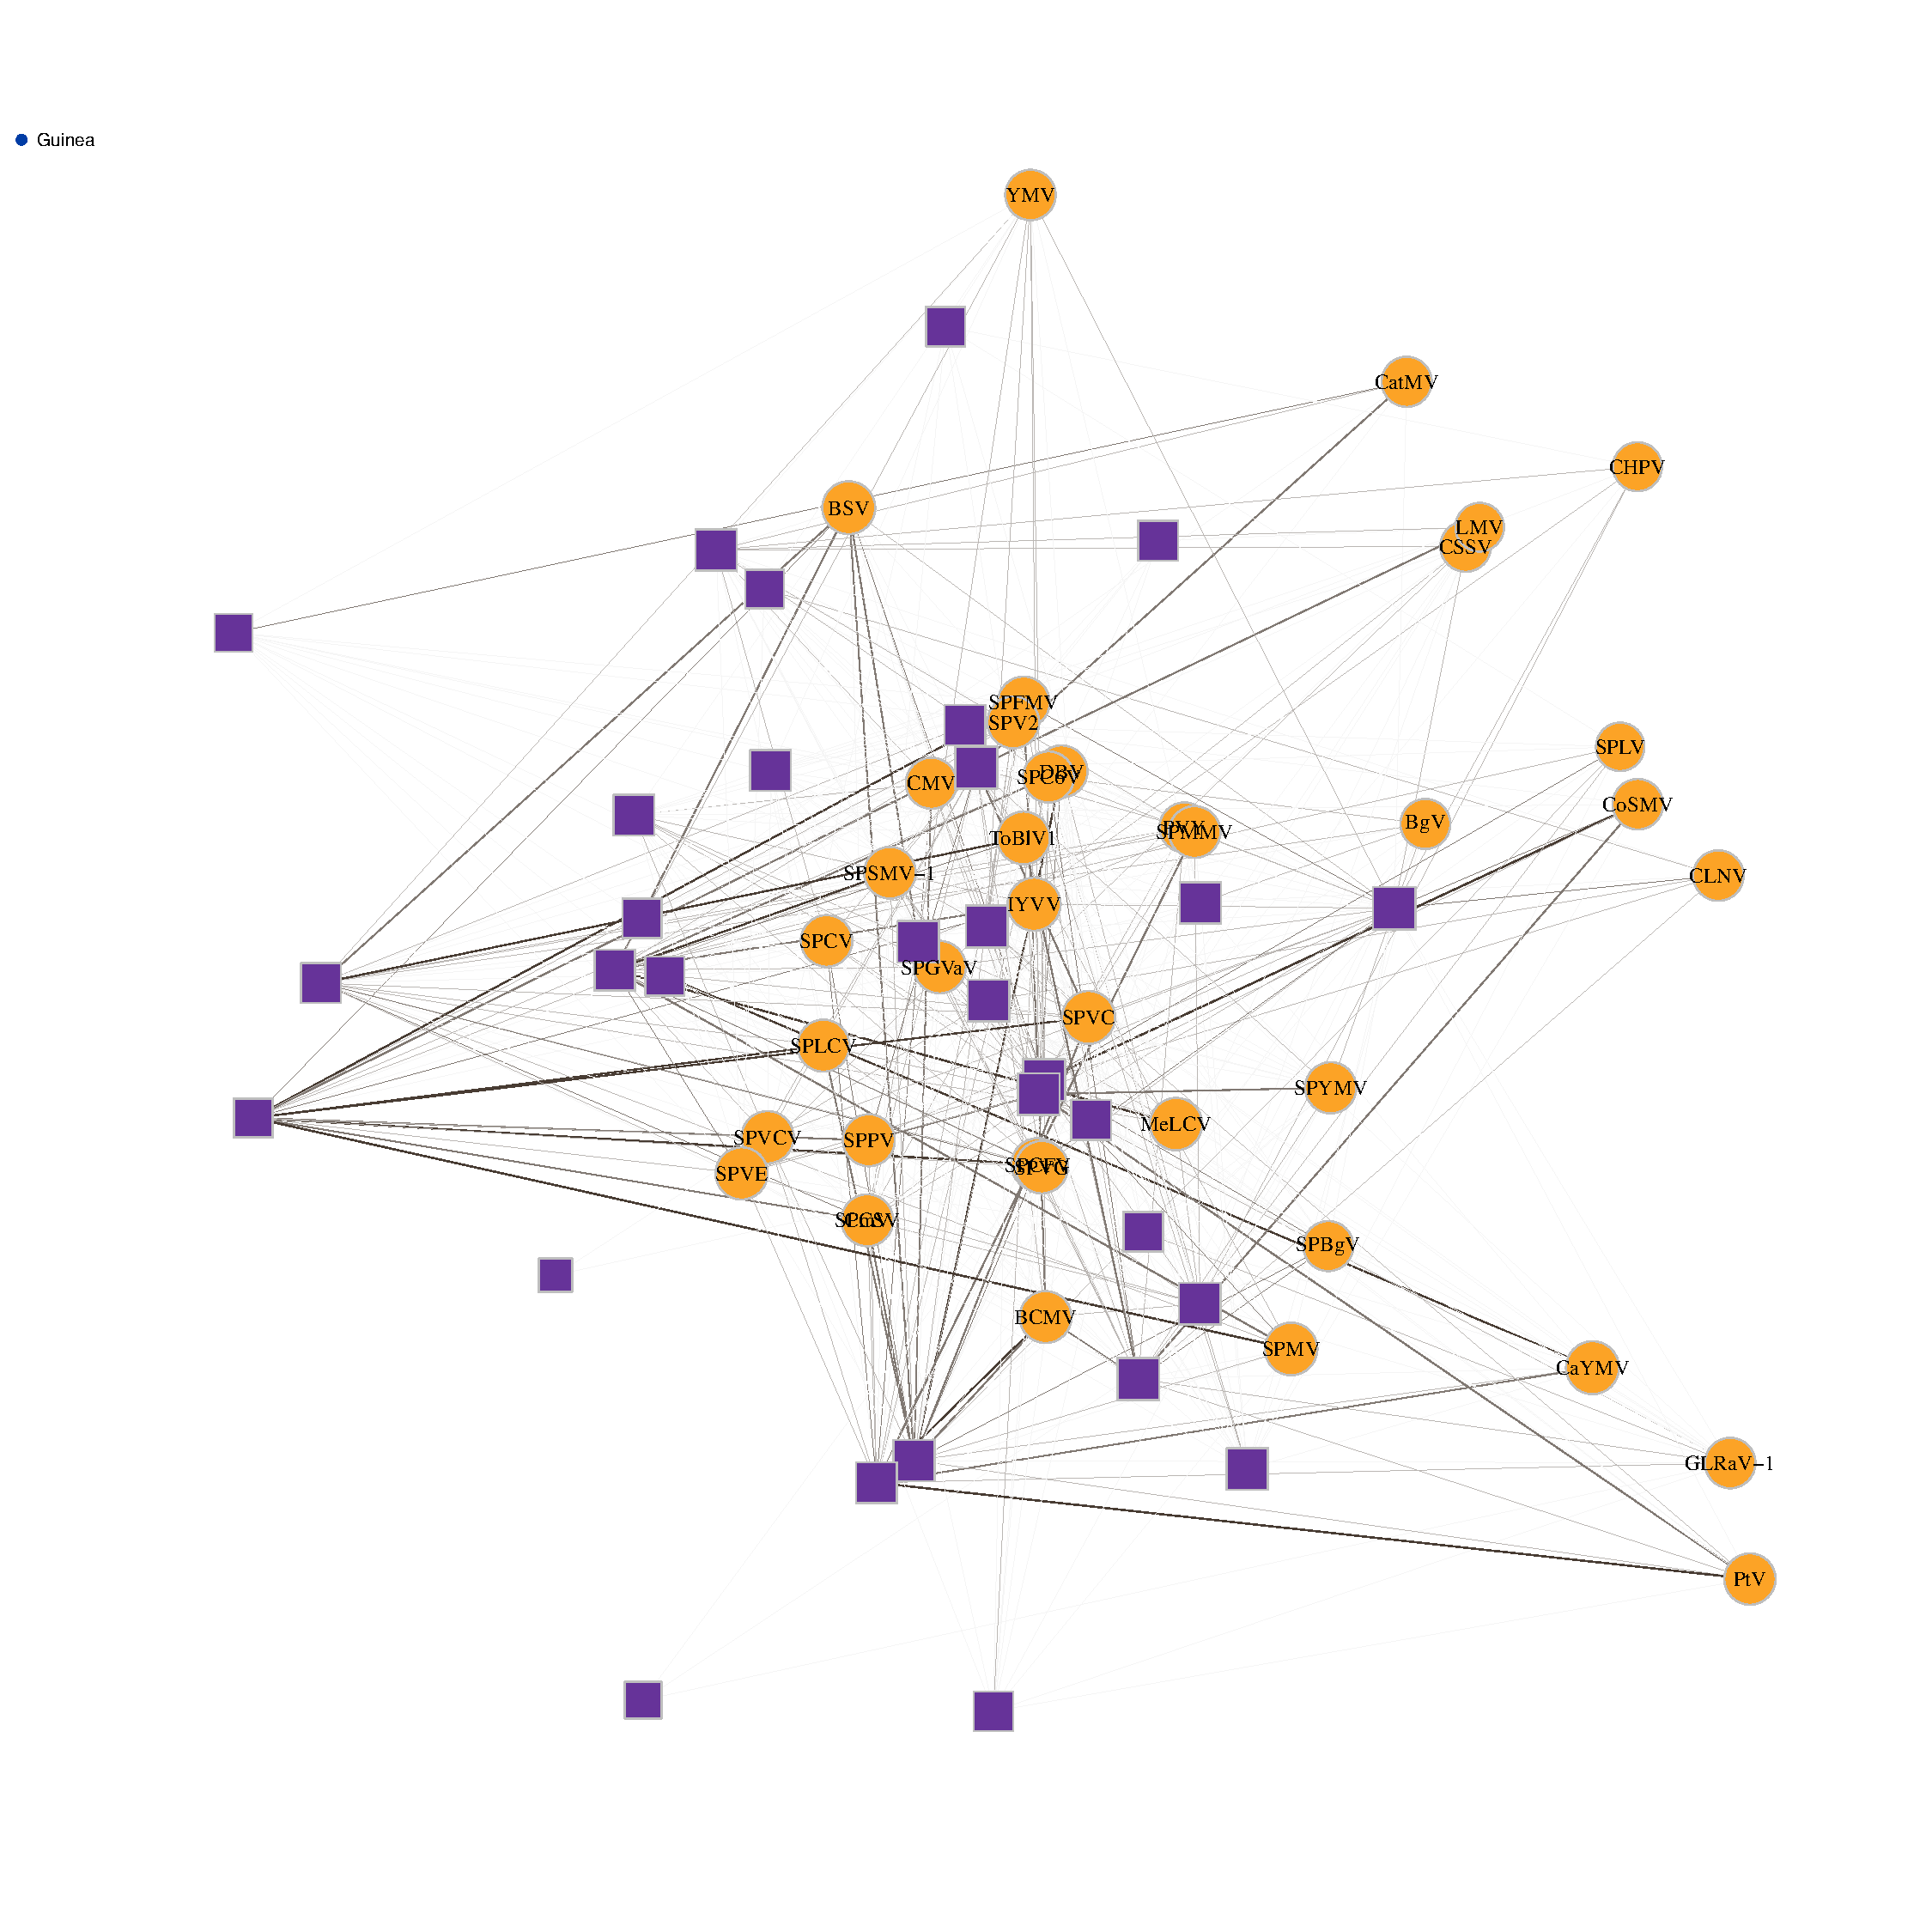
\includegraphics[width=0.85\textwidth]{../results/k-cluster2/2-kcluster_bipartitenetwork-kk_Feb28.pdf
} % Include the image placeholder.png
\caption{Bipartite network Sub-Saharan Africa sweetpotato virome region 1, Kimura-Kawai layout}
\end{center}
\end{figure}

\subsection{Region 3}

\begin{figure}[h!]
\begin{center}
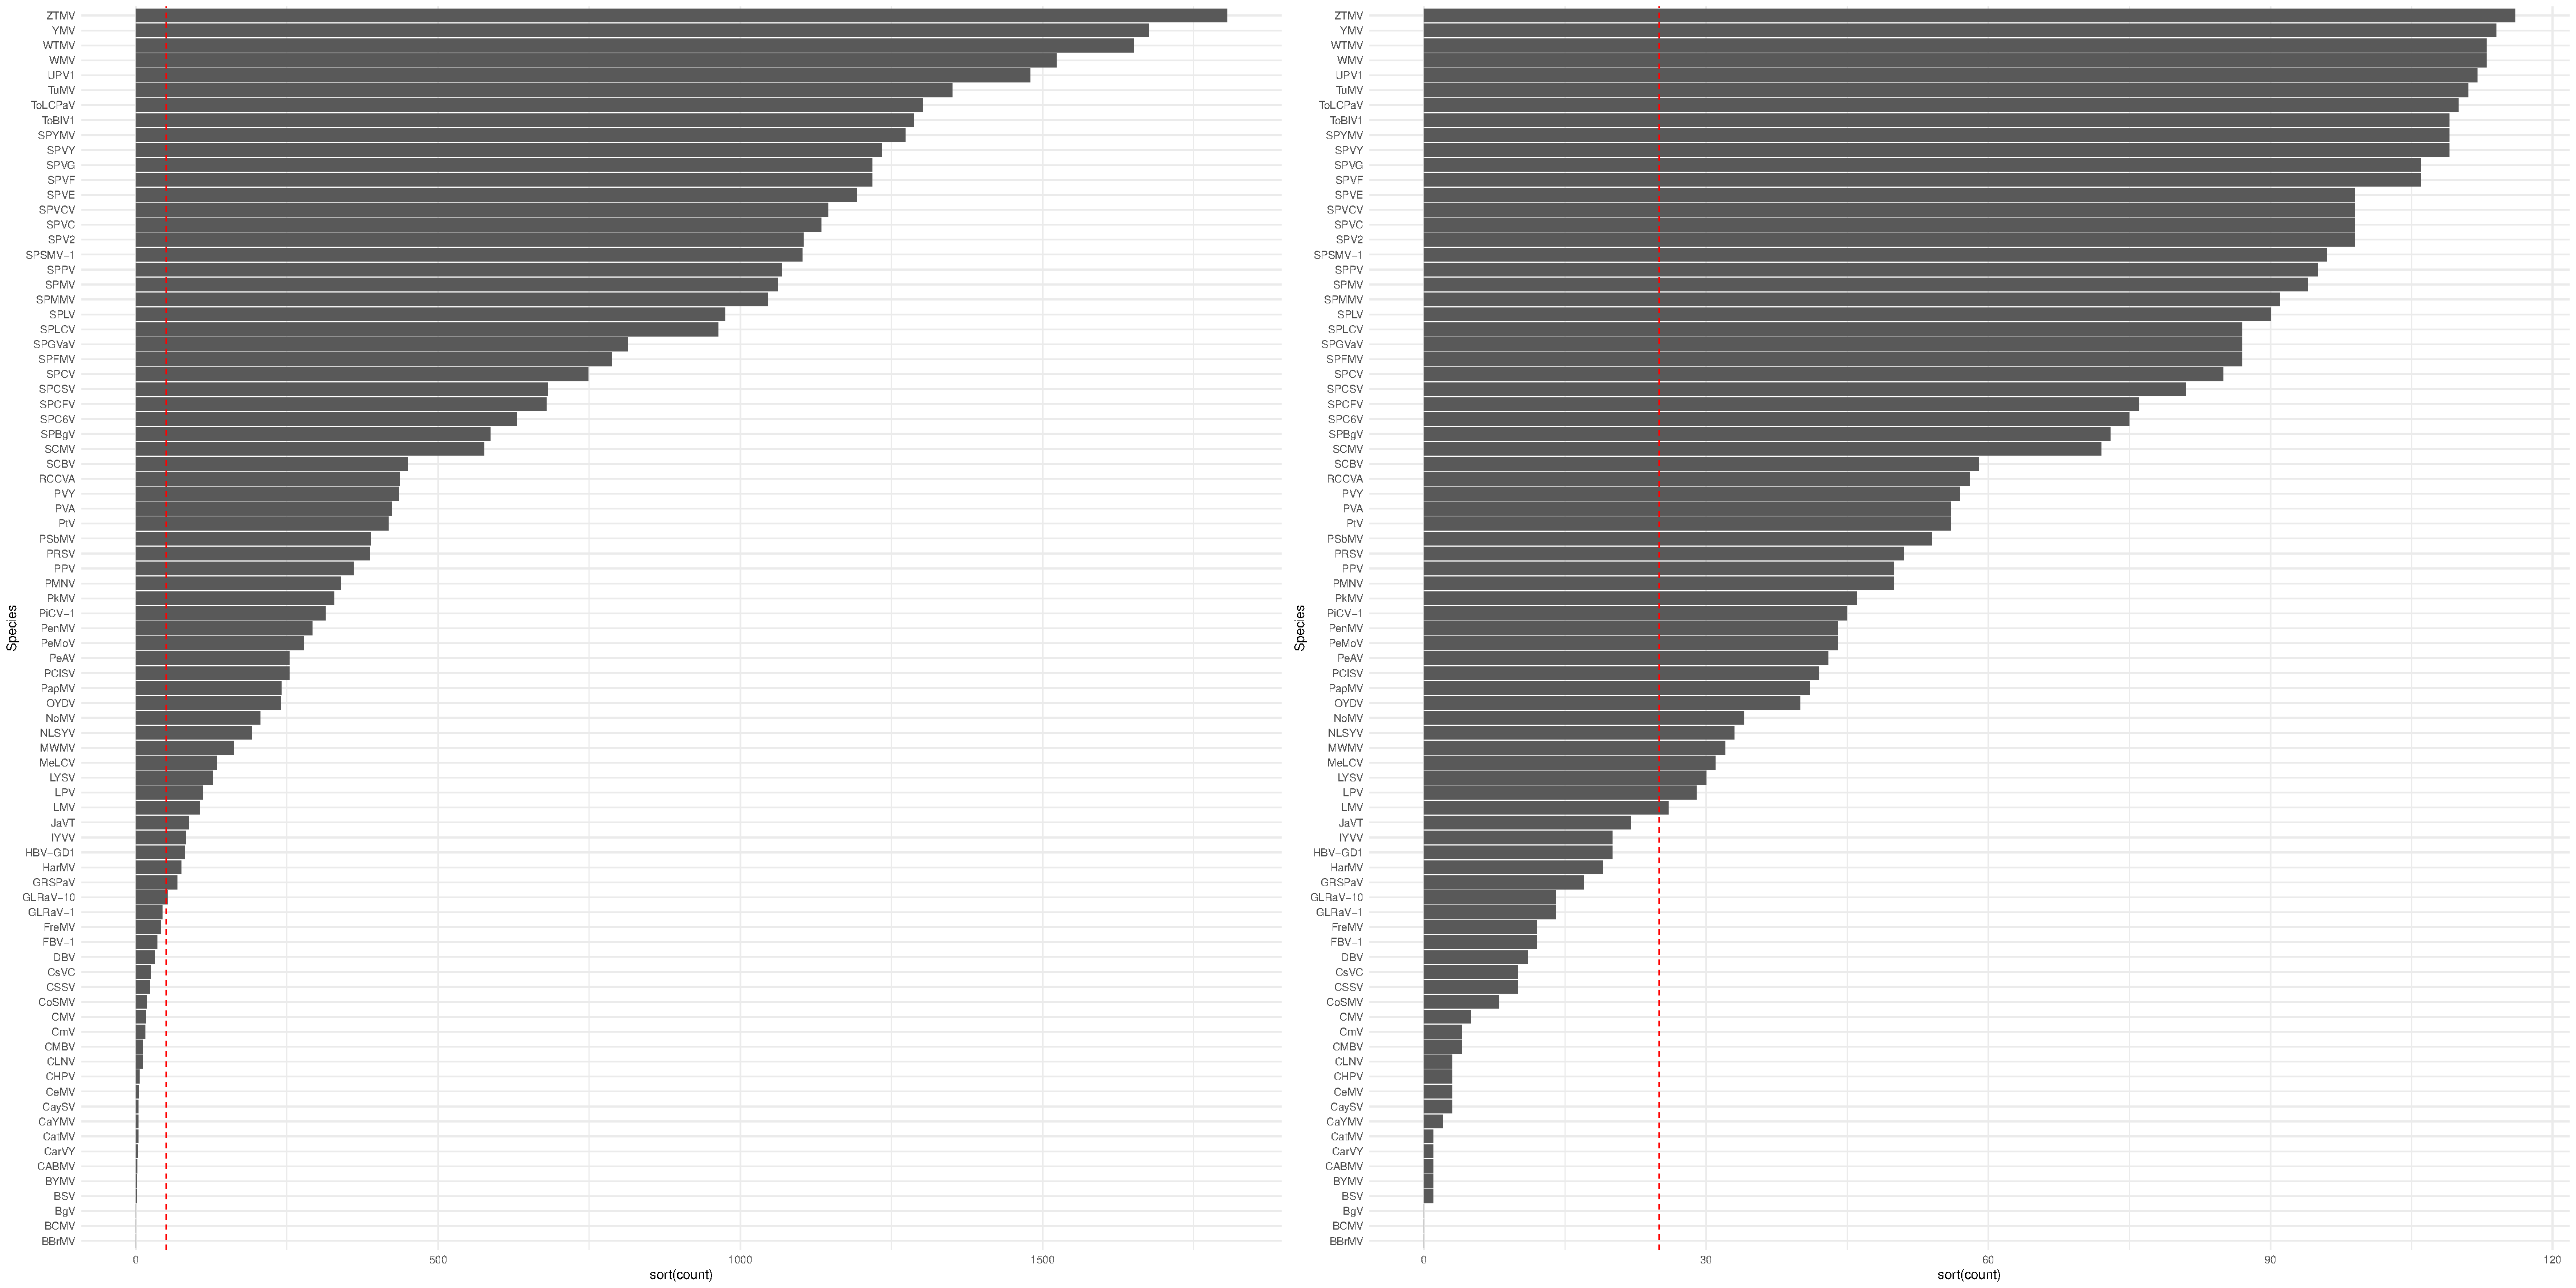
\includegraphics[width=0.95\textwidth]{../results/k-cluster3/3-kcluster_incidence_w+bFeb28.pdf
} % Include the image placeholder.png
\caption{Incidence distribution Sub-Saharan Africa sweetpotato virome region 1.}
\end{center}
\end{figure}


\begin{figure}[h!]
\begin{center}
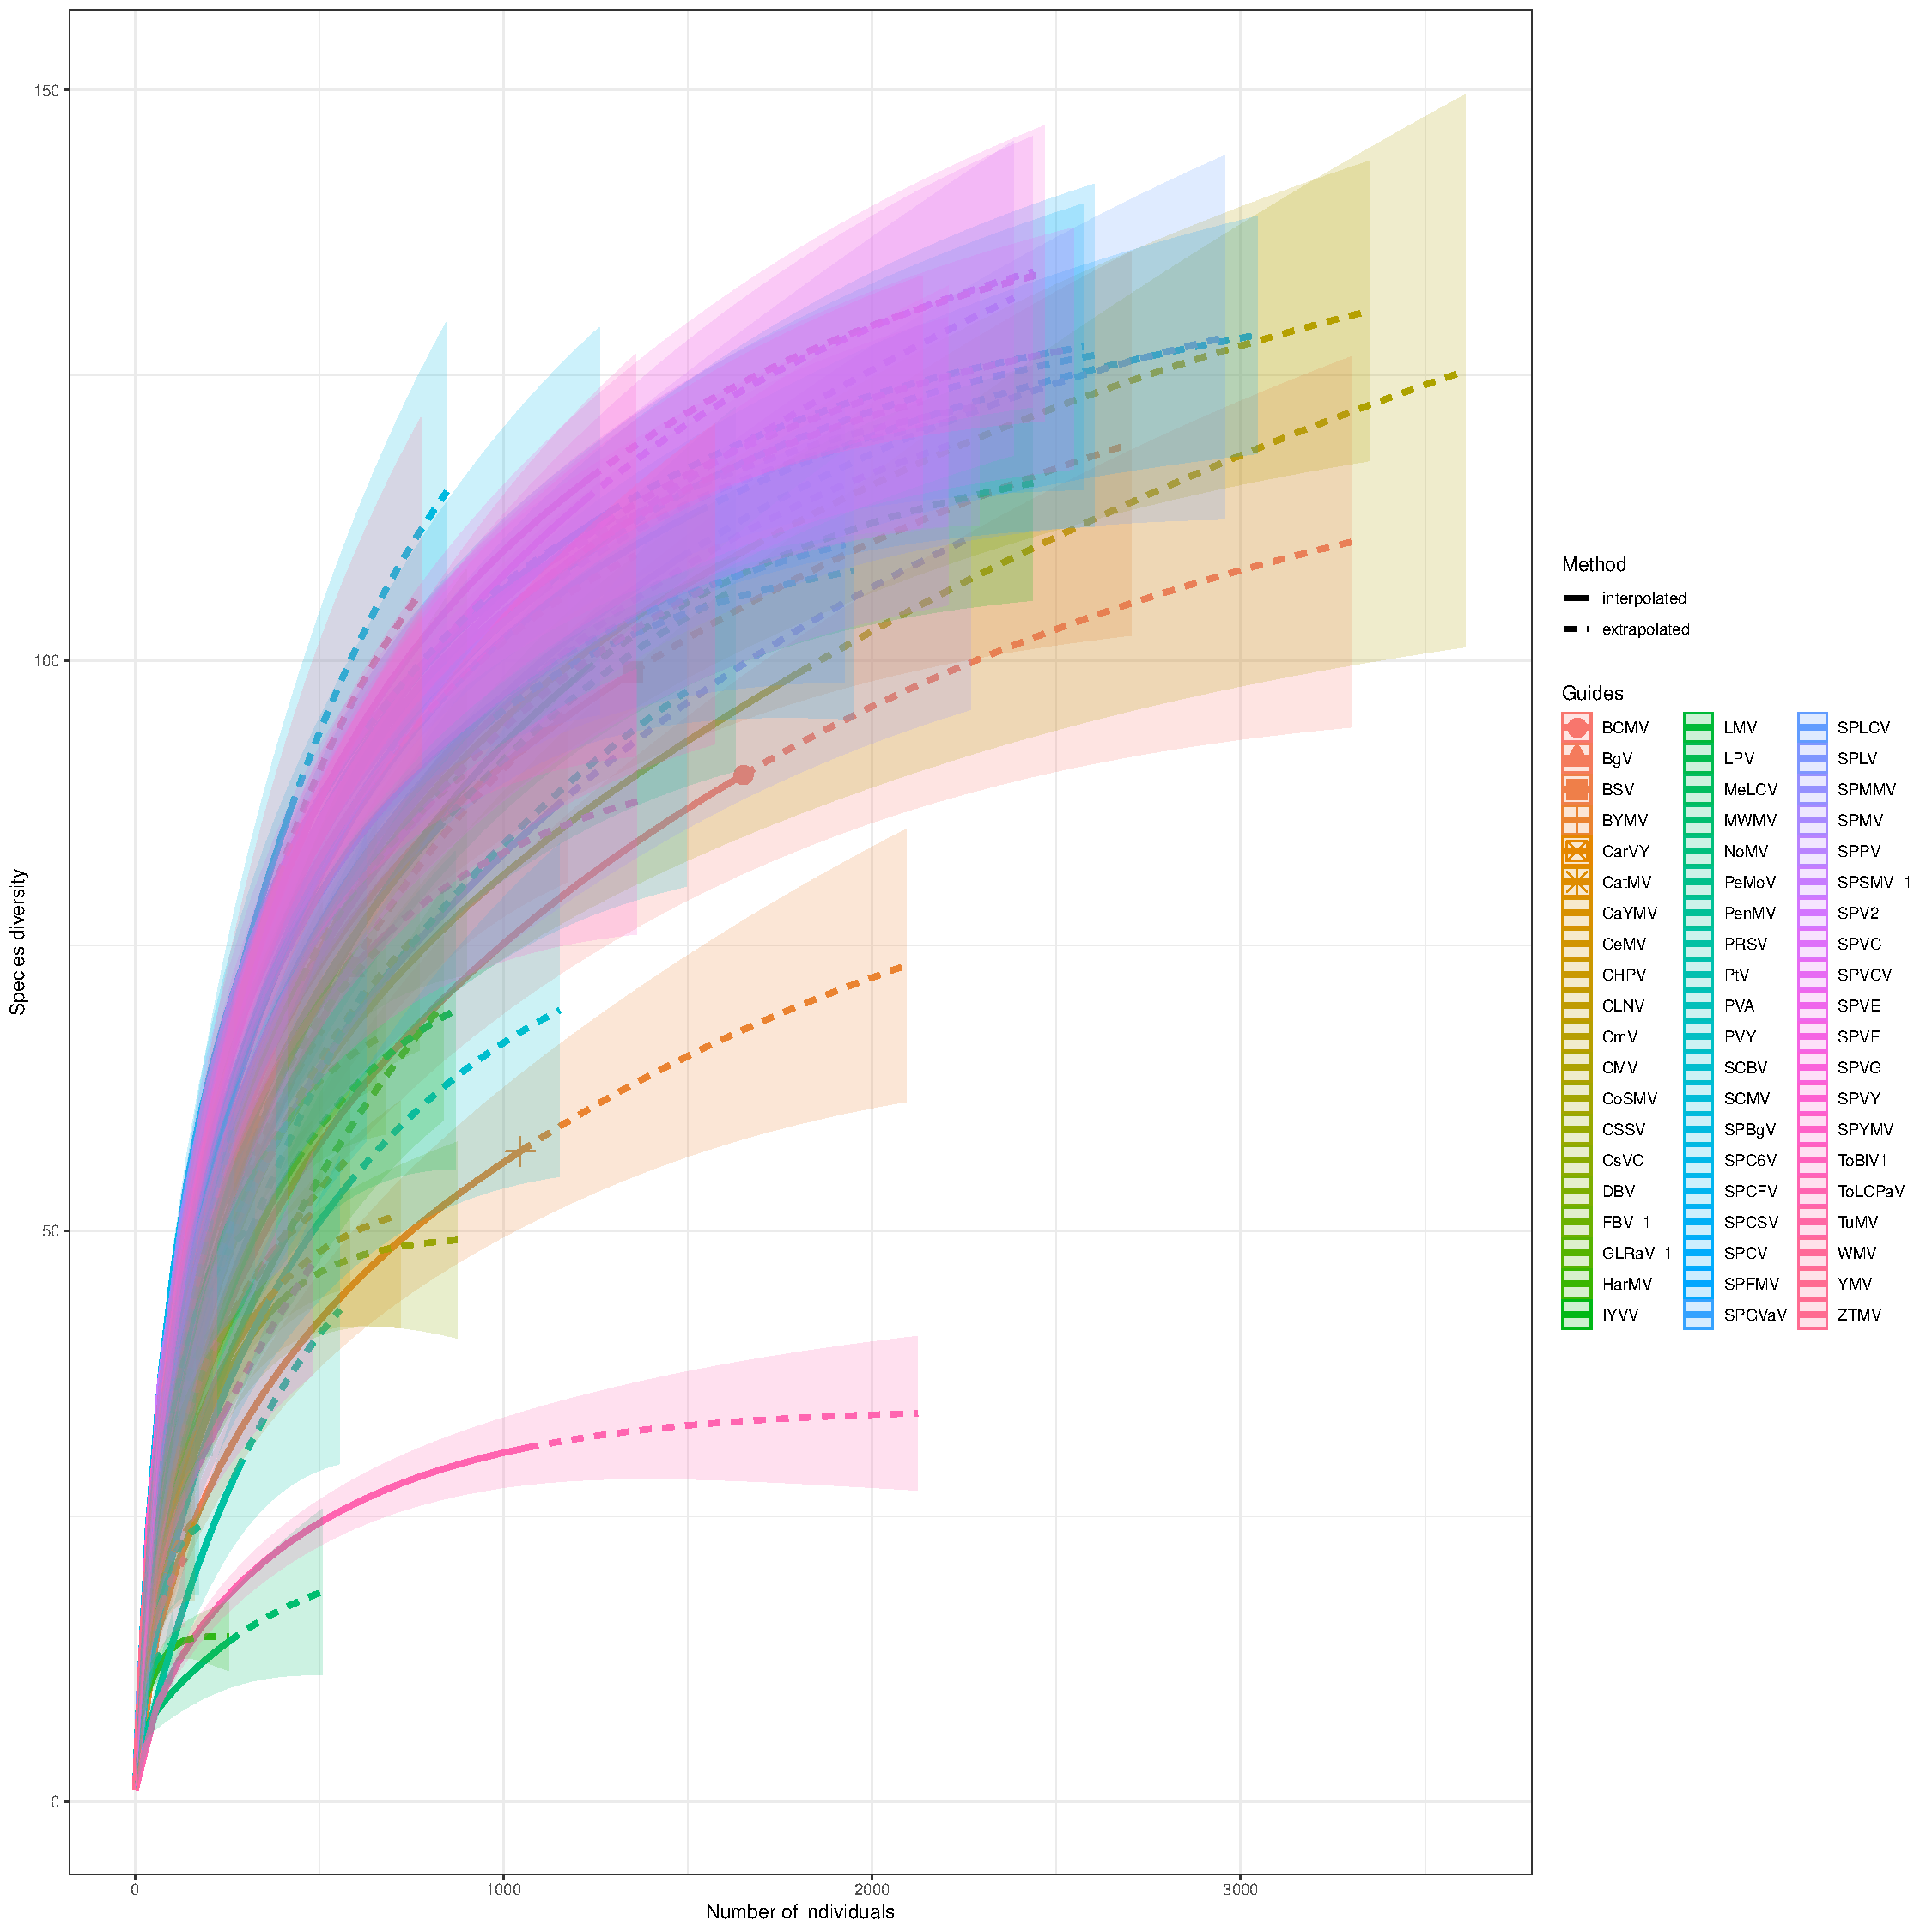
\includegraphics[width=0.75\textwidth]{../results/k-cluster3/3-kcluster_rarefaction-iNEXT_Feb28.pdf
} % Include the image placeholder.png
\caption{Rarefaction of Sub-Saharan Africa sweetpotato virome region 1.}
\end{center}
\end{figure}


\begin{figure}[h!]
\begin{center}
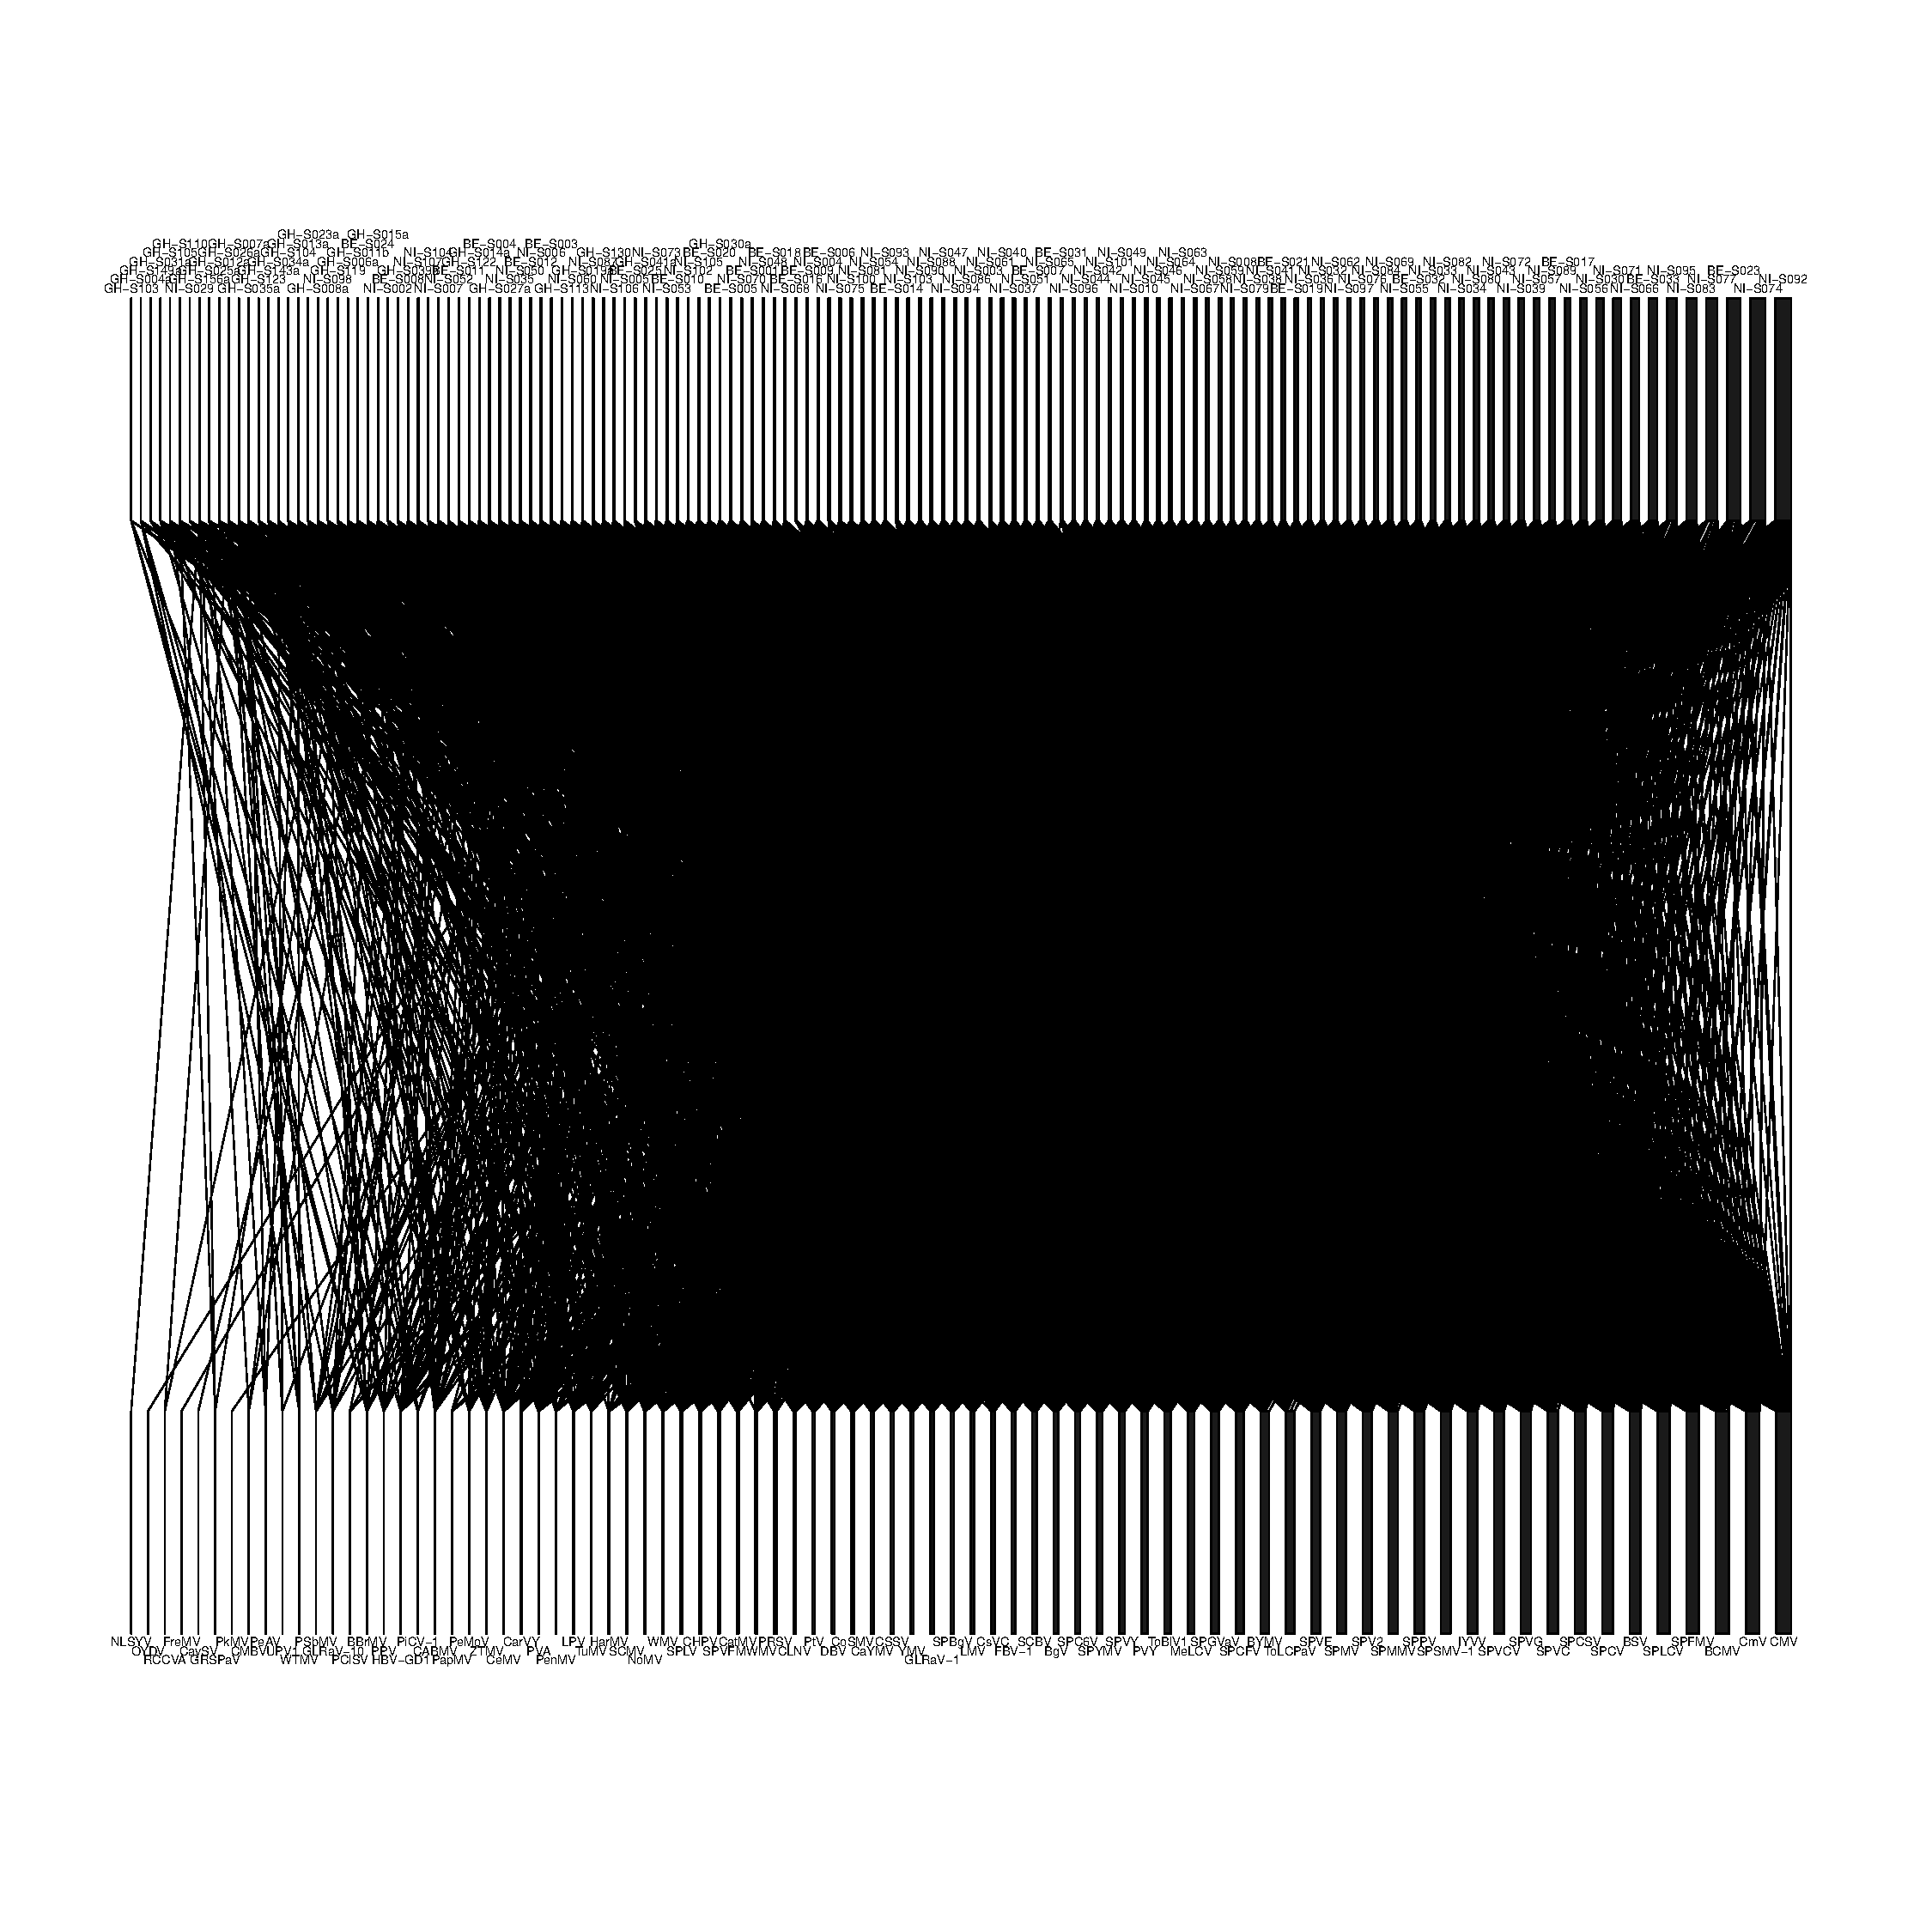
\includegraphics[width=0.75\textwidth]{../results/k-cluster3/3-kcluster_bipartitenetwork_Feb28.pdf
} % Include the image placeholder.png
\caption{Bipartite network Sub-Saharan Africa sweetpotato virome region 1.}
\end{center}
\end{figure}



\begin{figure}[h!]
\begin{center}
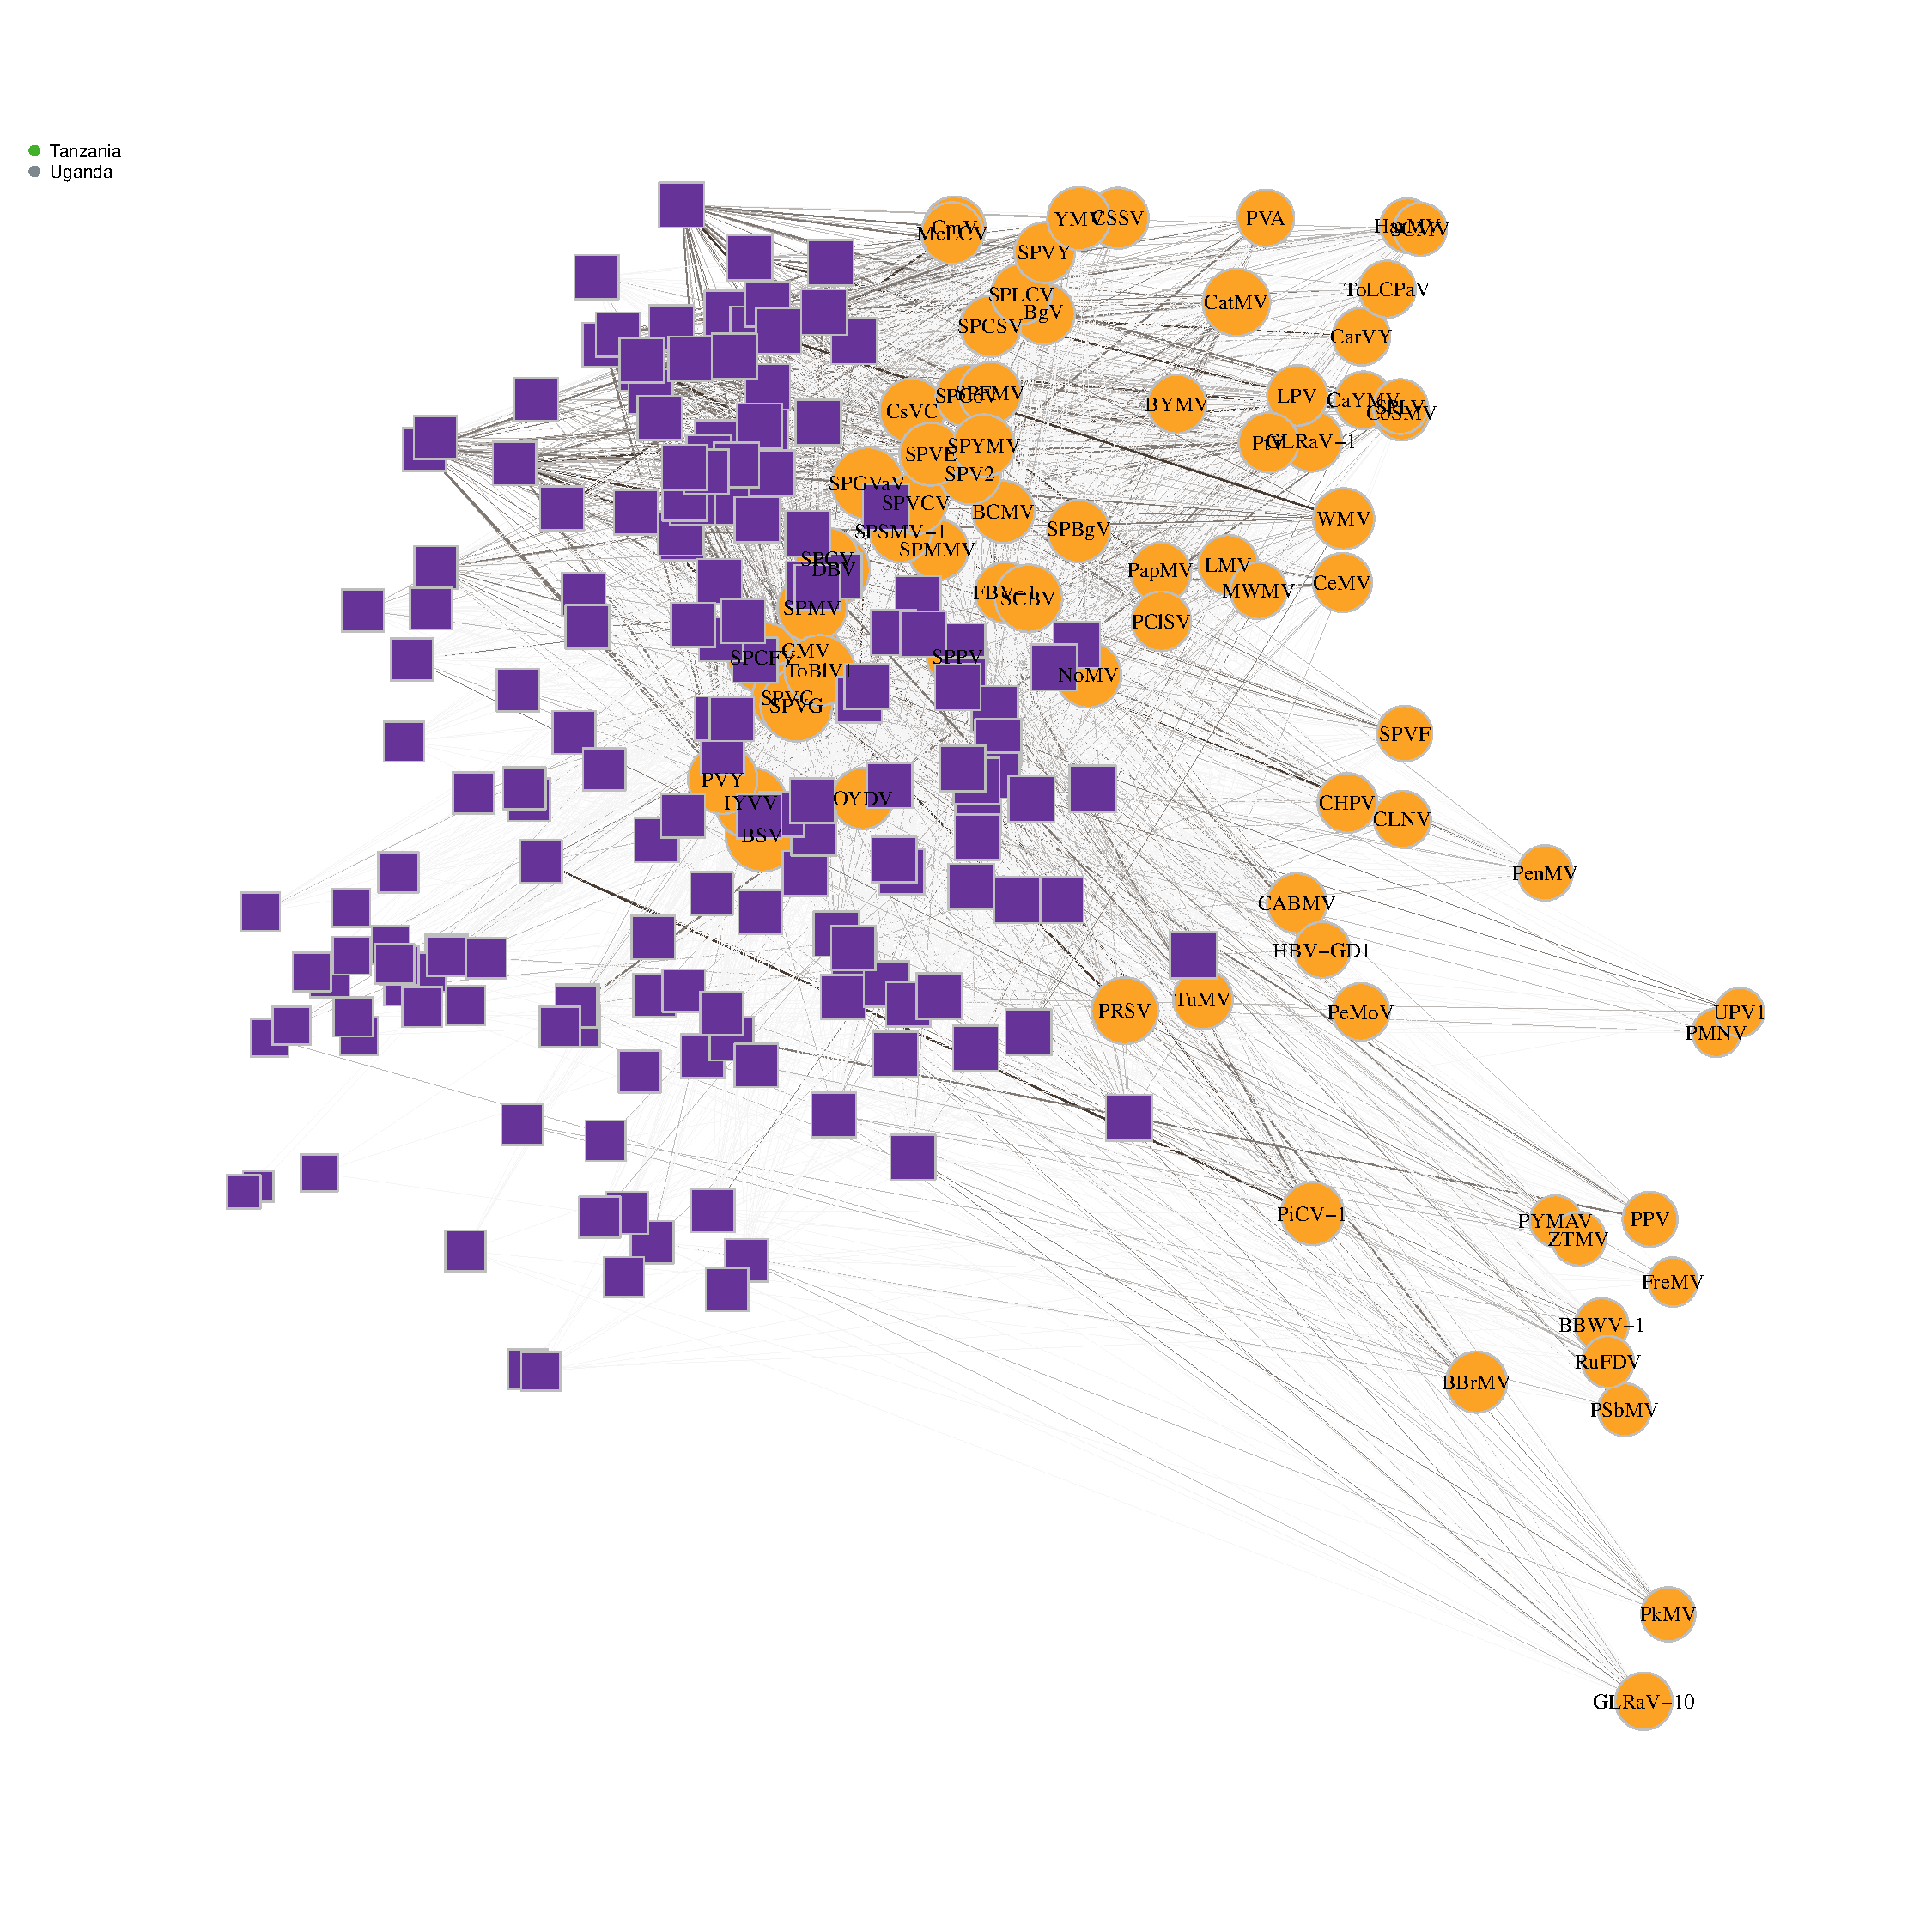
\includegraphics[width=0.85\textwidth]{../results/k-cluster1/1-kcluster_bipartitenetwork-kk_Feb28.pdf
} % Include the image placeholder.png
\caption{Bipartite network Sub-Saharan Africa sweetpotato virome region 1, Kimura-Kawai layout}
\end{center}
\end{figure}

\subsection{Region 4}

\begin{figure}[h!]
\begin{center}
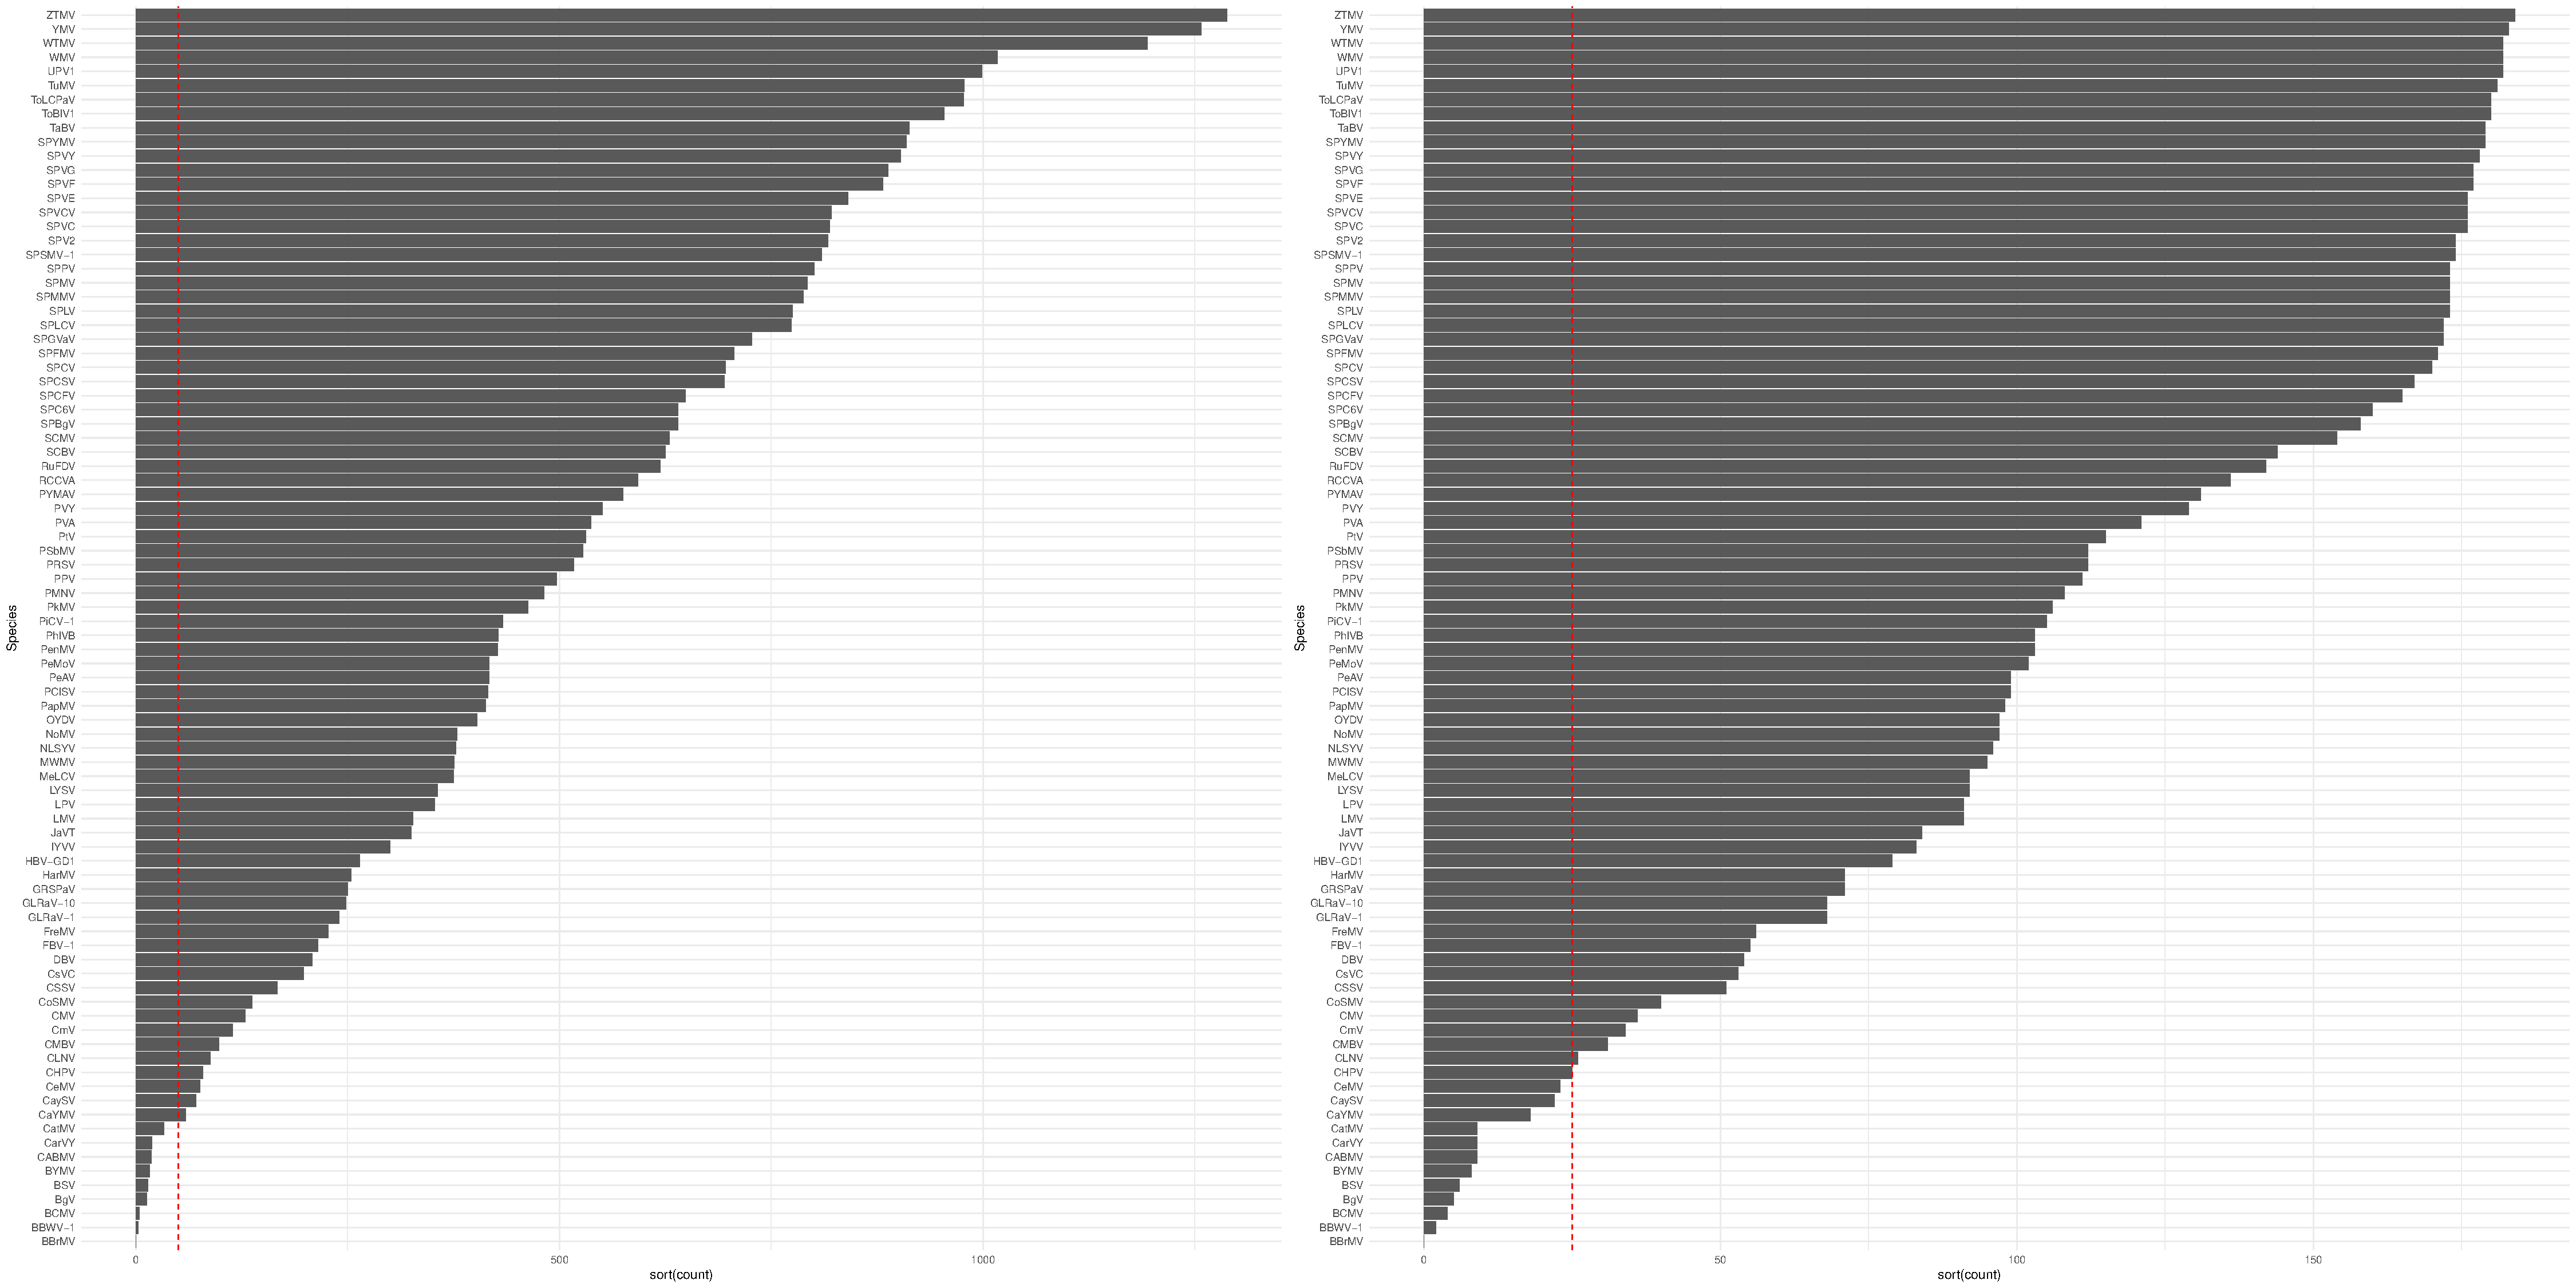
\includegraphics[width=0.95\textwidth]{../results/k-cluster4/4-kcluster_incidence_w+bFeb28.pdf
} % Include the image placeholder.png
\caption{Incidence distribution Sub-Saharan Africa sweetpotato virome region 1.}
\end{center}
\end{figure}


\begin{figure}[h!]
\begin{center}
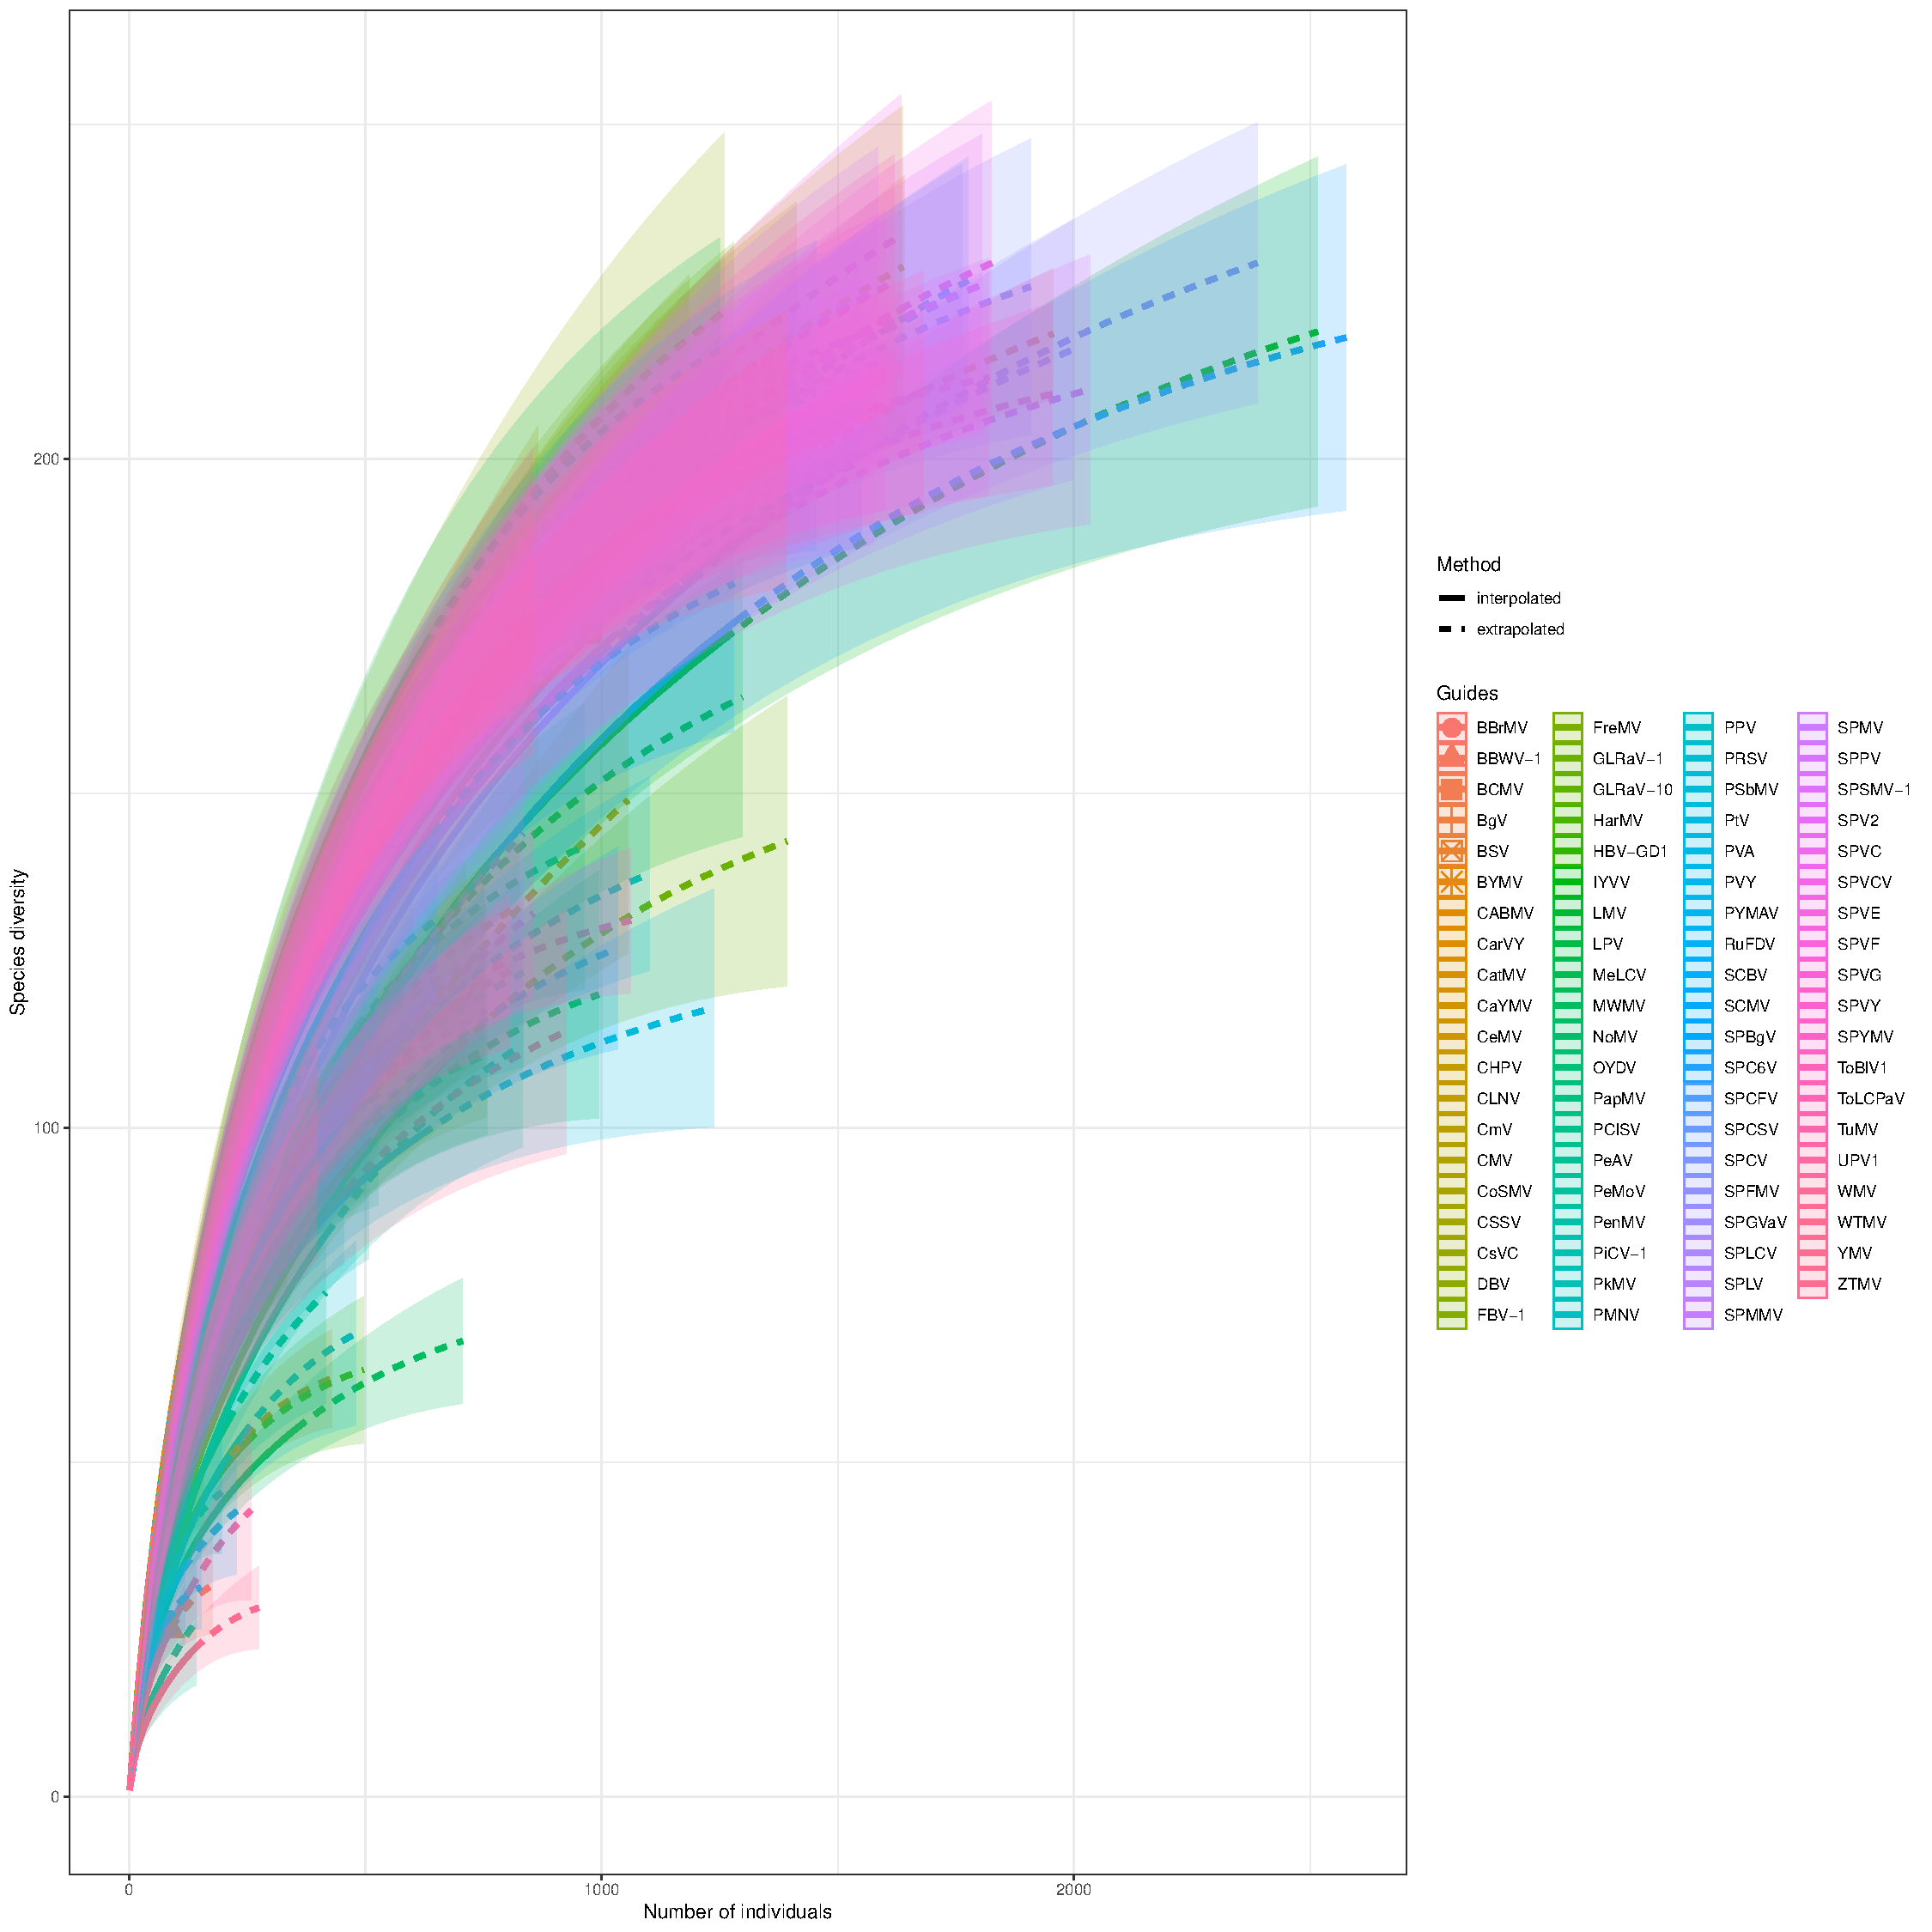
\includegraphics[width=0.75\textwidth]{../results/k-cluster4/4-kcluster_rarefaction-iNEXT_Feb28.pdf
} % Include the image placeholder.png
\caption{Rarefaction of Sub-Saharan Africa sweetpotato virome region 1.}
\end{center}
\end{figure}


\begin{figure}[h!]
\begin{center}
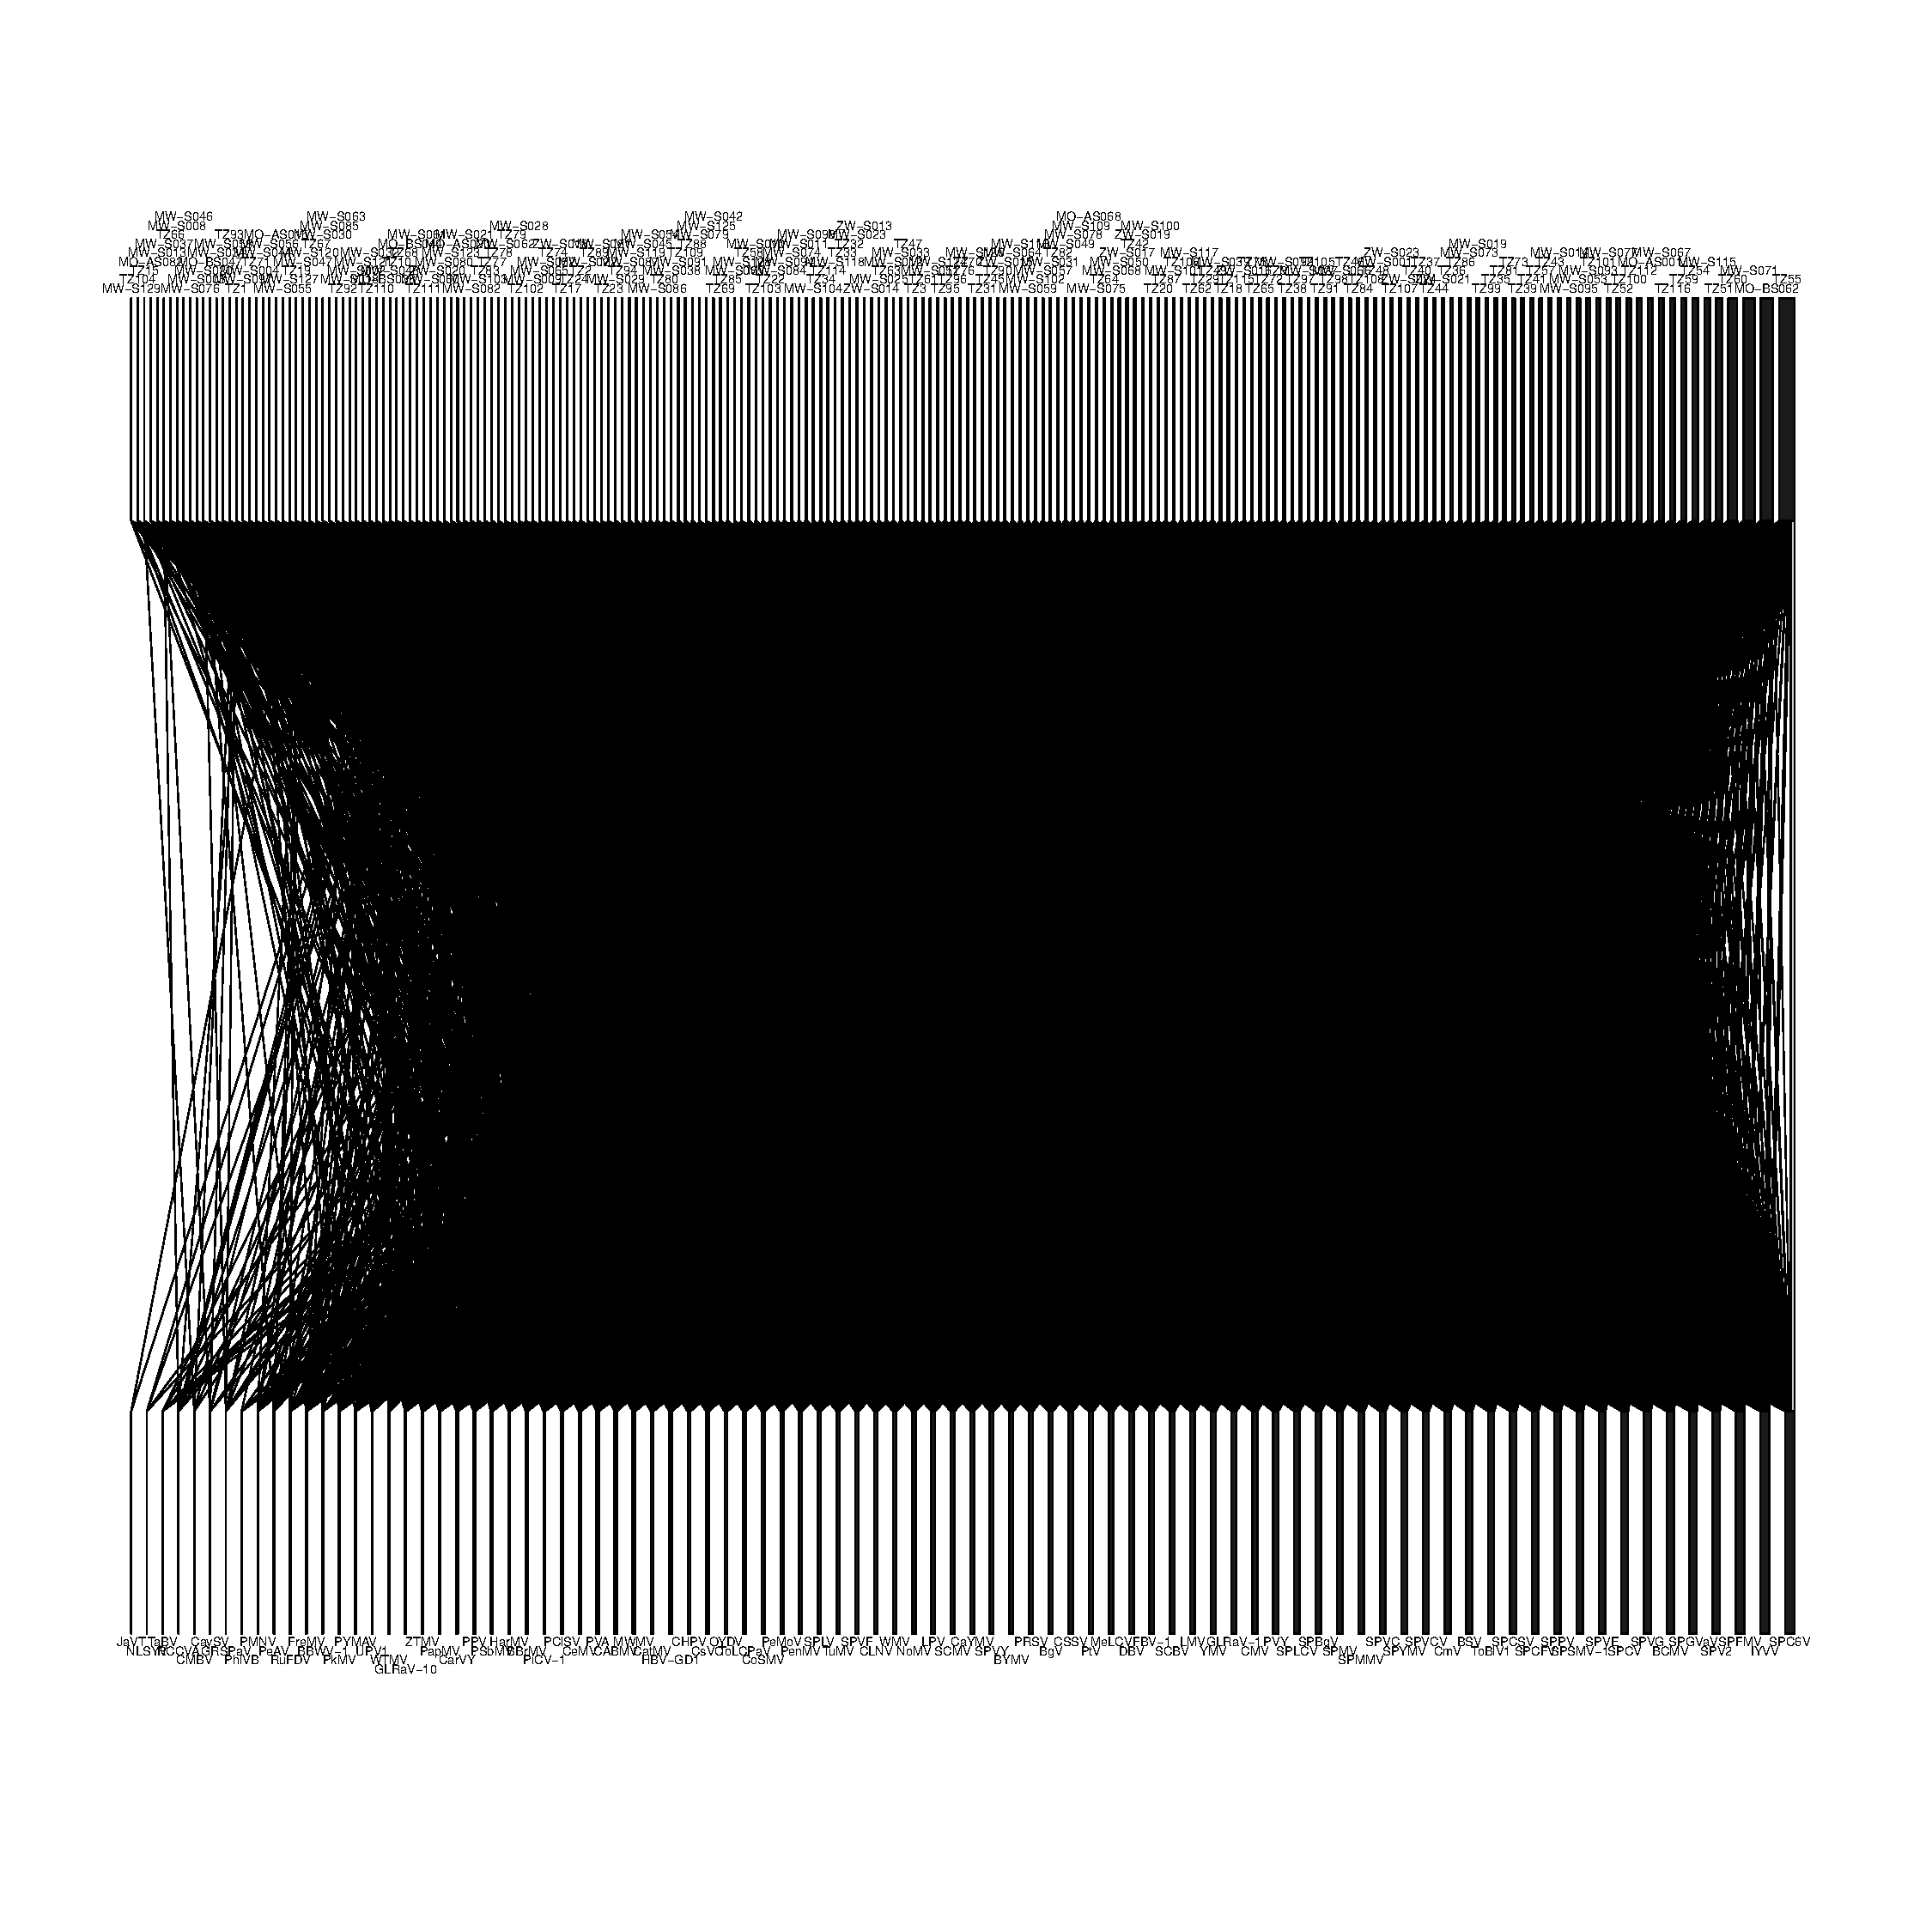
\includegraphics[width=0.75\textwidth]{../results/k-cluster4/4-kcluster_bipartitenetwork_Feb28.pdf
} % Include the image placeholder.png
\caption{Bipartite network Sub-Saharan Africa sweetpotato virome region 1.}
\end{center}
\end{figure}



\begin{figure}[h!]
\begin{center}
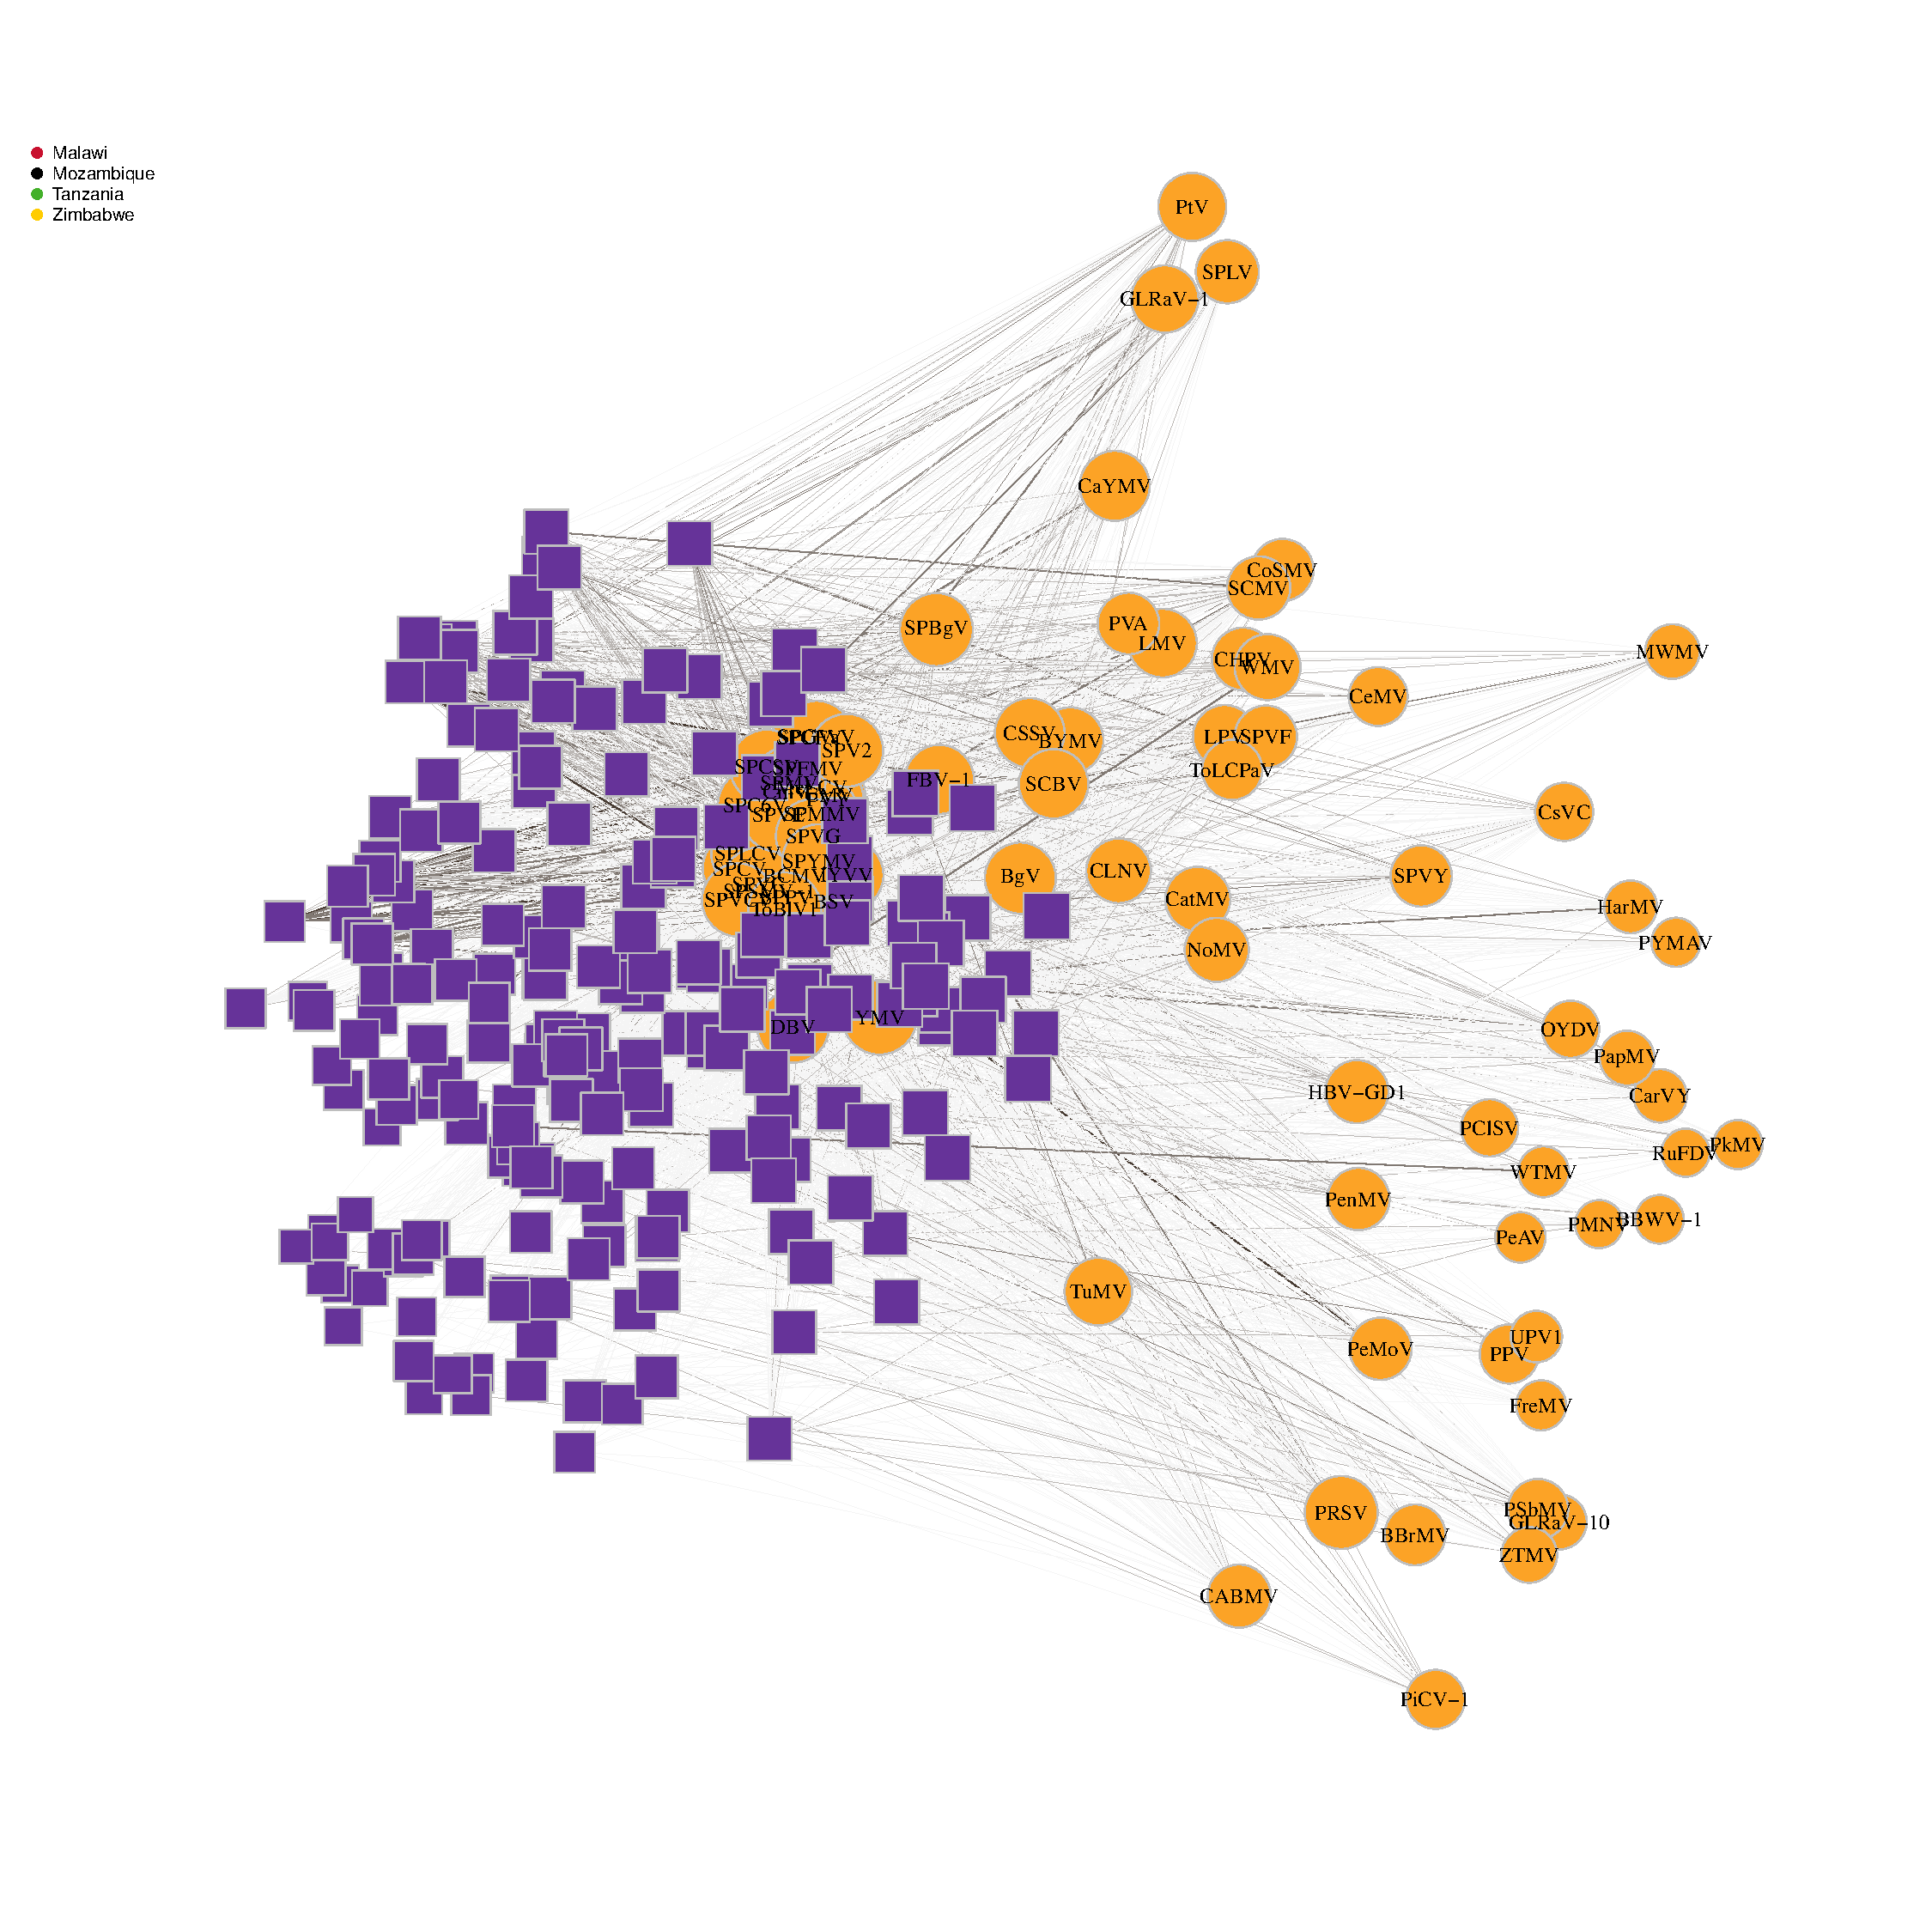
\includegraphics[width=0.85\textwidth]{../results/k-cluster4/4-kcluster_bipartitenetwork-kk_Feb28.pdf
} % Include the image placeholder.png
\caption{Bipartite network Sub-Saharan Africa sweetpotato virome region 1, Kimura-Kawai layout}
\end{center}
\end{figure}

\subsection{Region 5}

\begin{figure}[h!]
\begin{center}
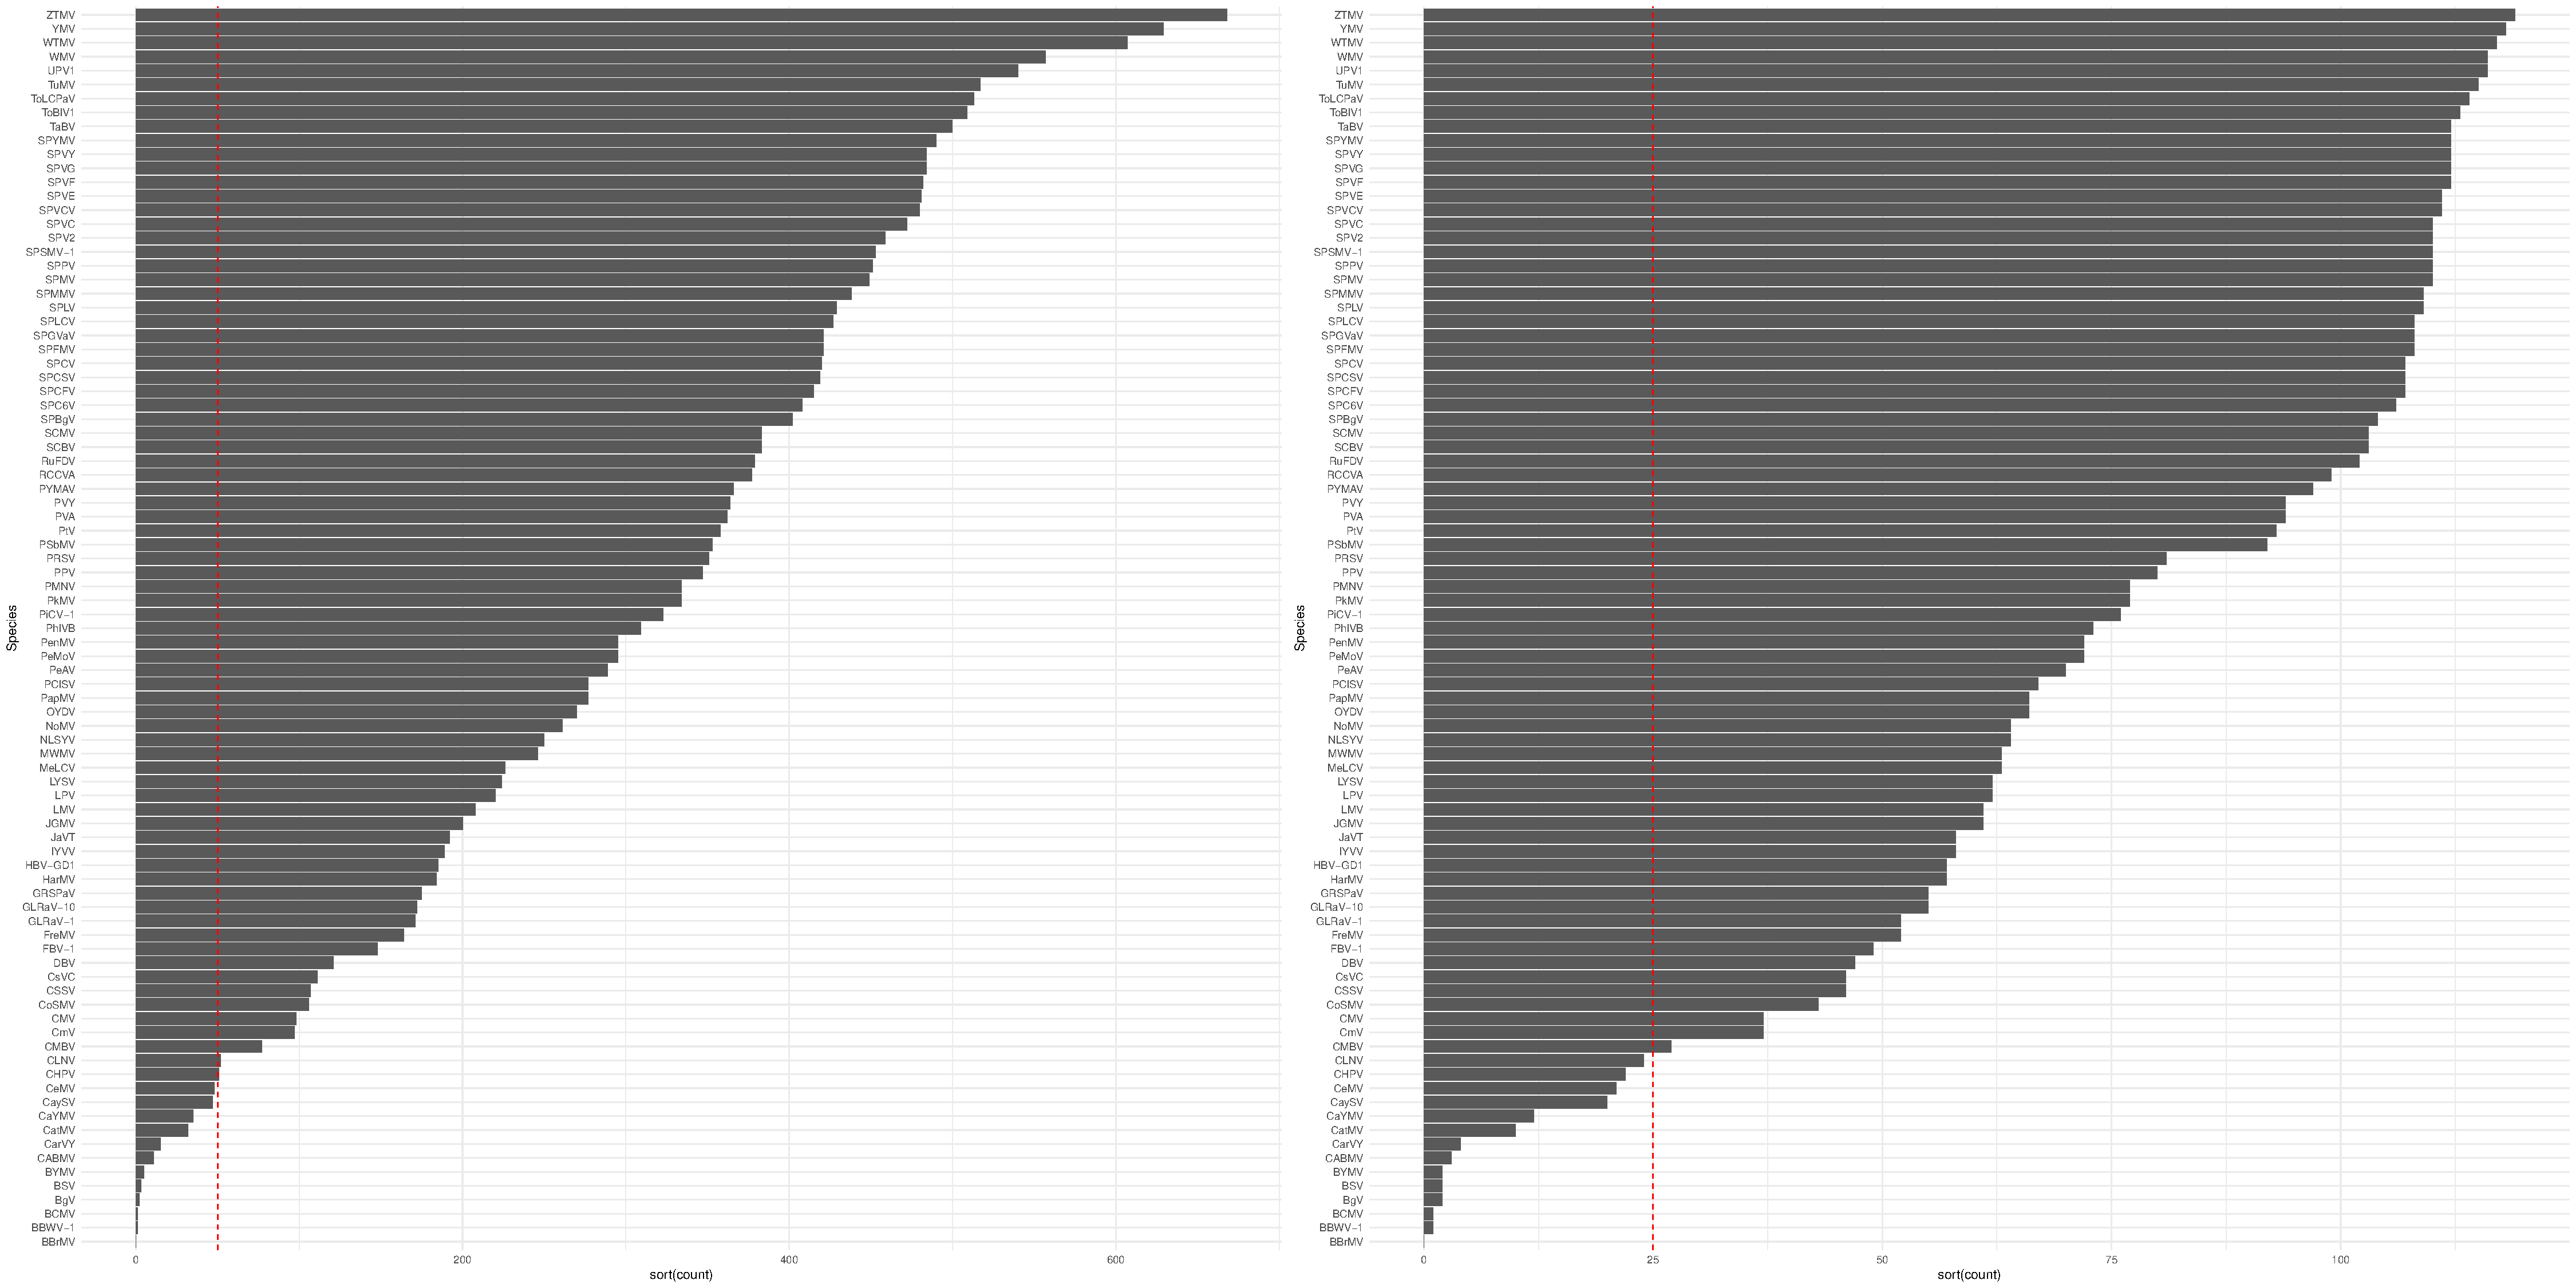
\includegraphics[width=0.95\textwidth]{../results/k-cluster5/5-kcluster_incidence_w+bFeb28.pdf
} % Include the image placeholder.png
\caption{Incidence distribution Sub-Saharan Africa sweetpotato virome region 1.}
\end{center}
\end{figure}


\begin{figure}[h!]
\begin{center}
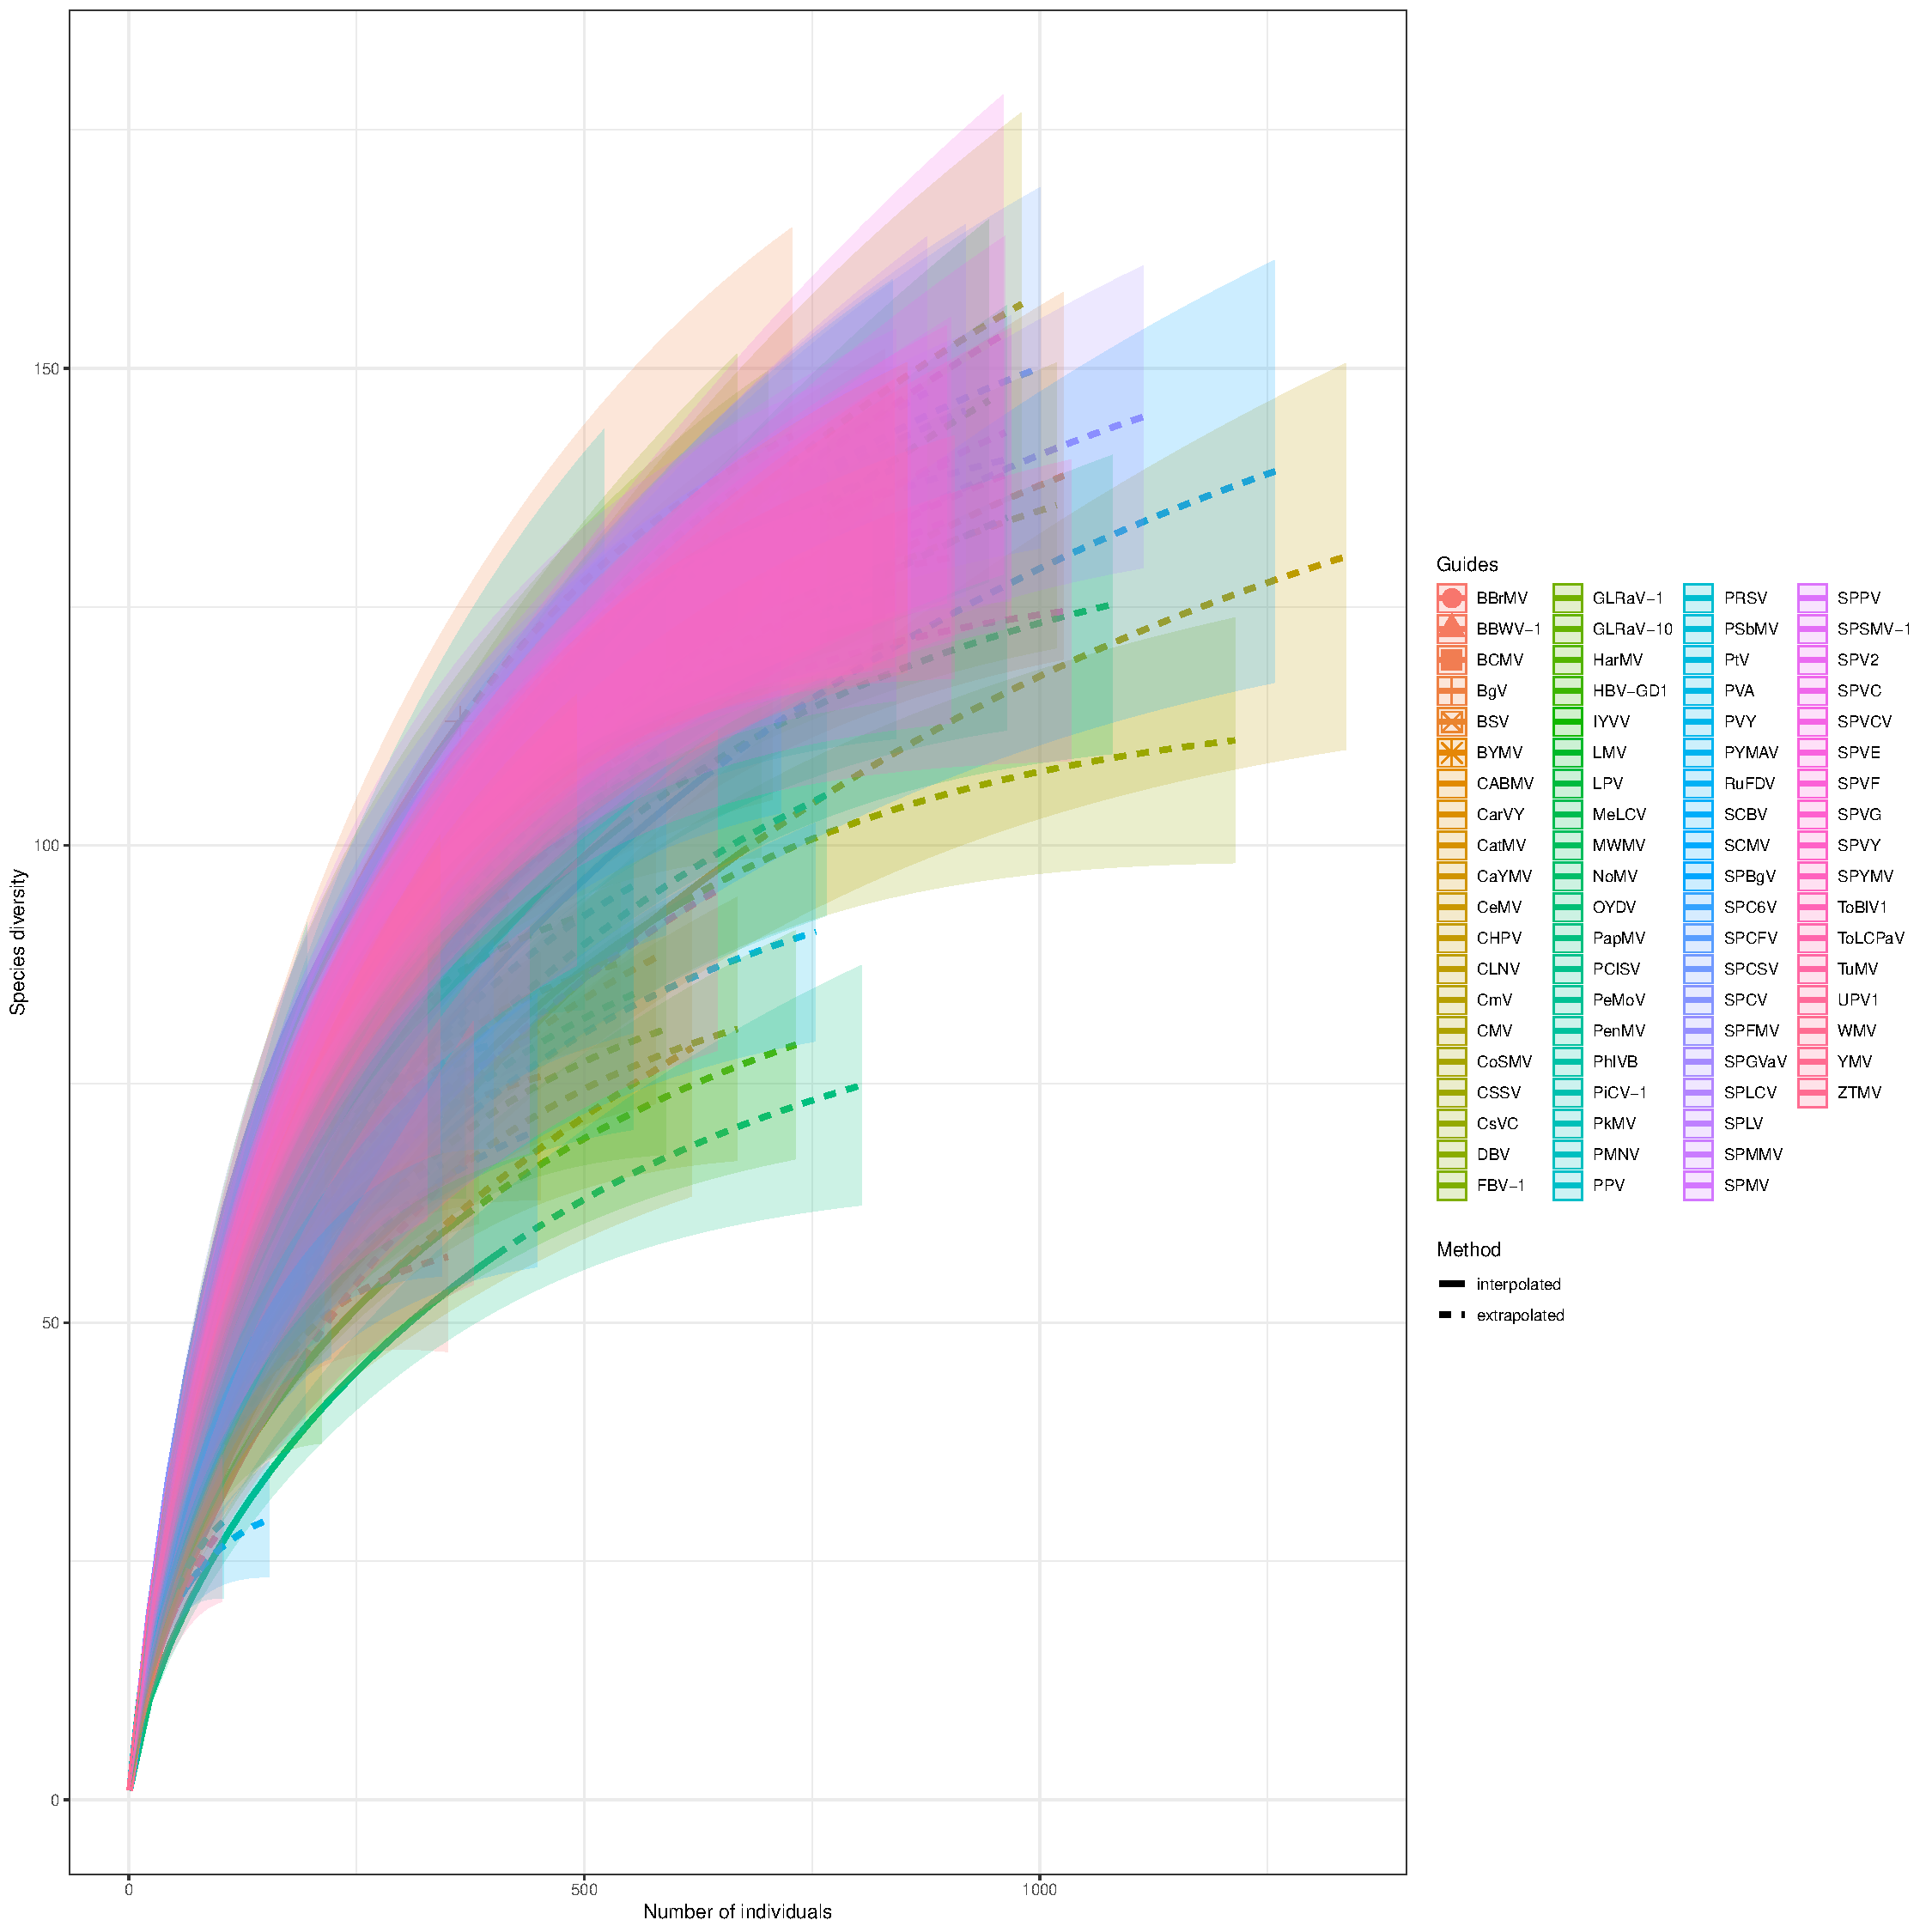
\includegraphics[width=0.75\textwidth]{../results/k-cluster5/5-kcluster_rarefaction-iNEXT_Feb28.pdf
} % Include the image placeholder.png
\caption{Rarefaction of Sub-Saharan Africa sweetpotato virome region 1.}
\end{center}
\end{figure}


\begin{figure}[h!]
\begin{center}
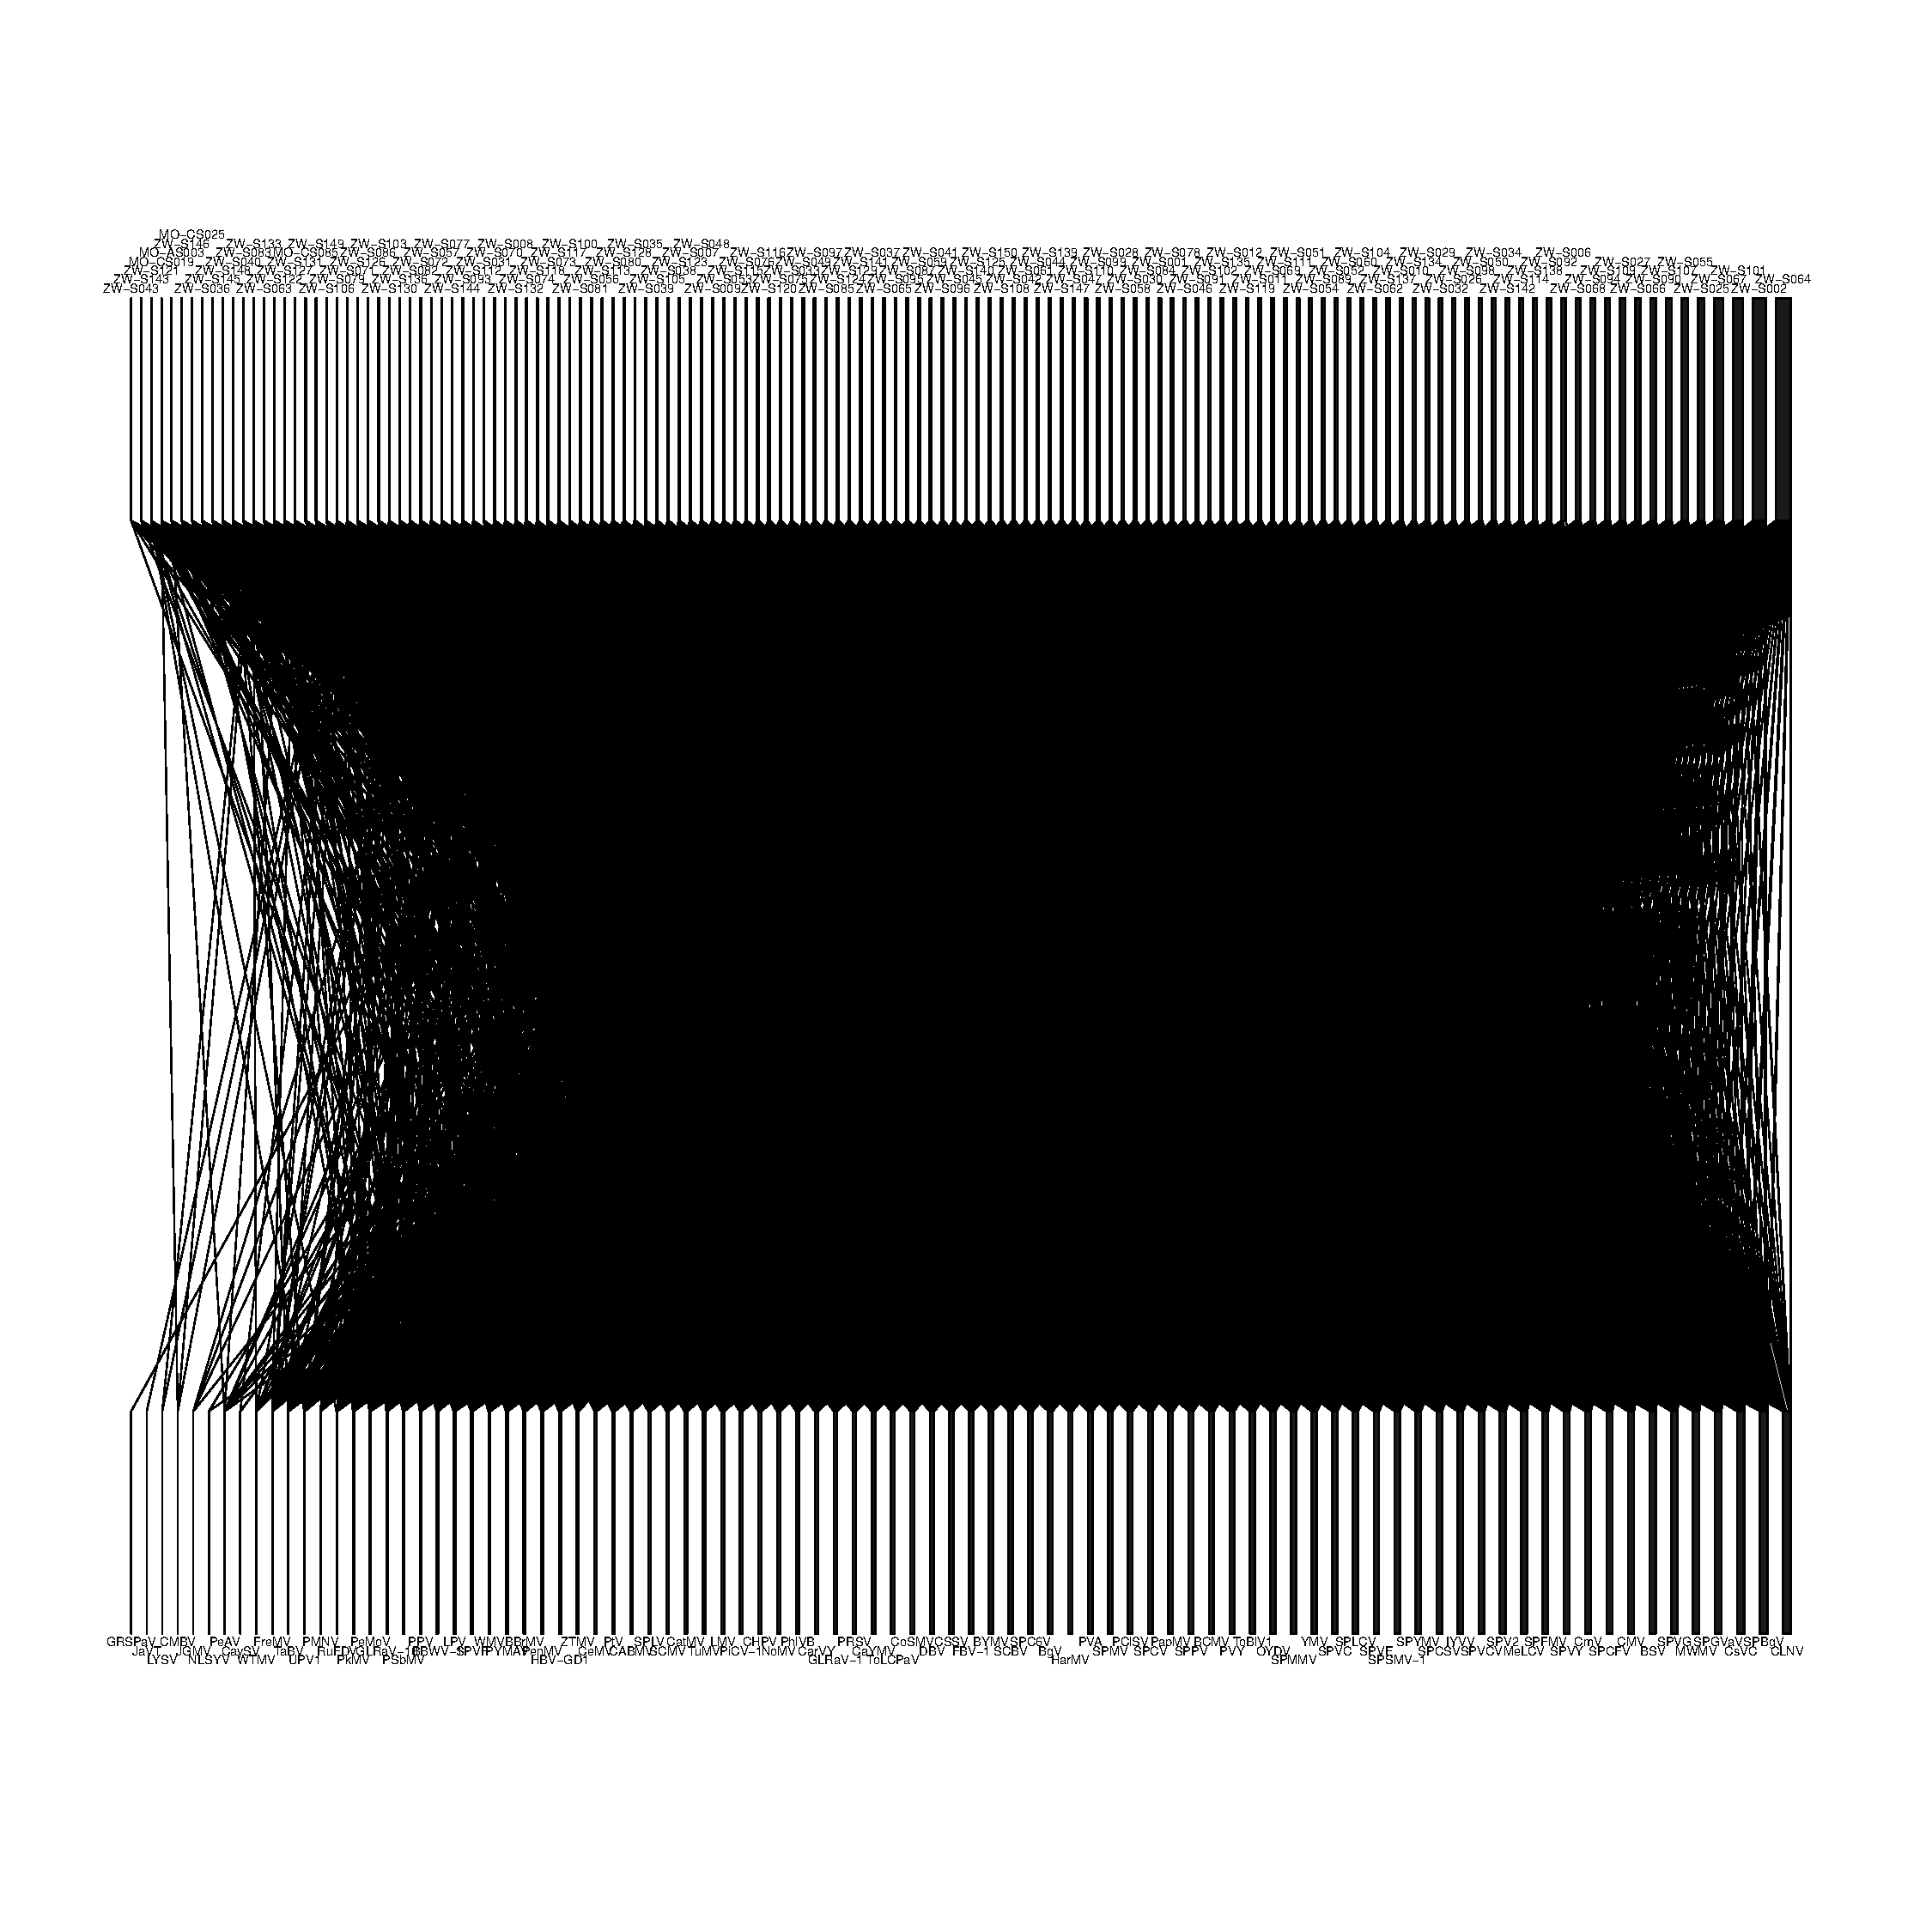
\includegraphics[width=0.75\textwidth]{../results/k-cluster5/5-kcluster_bipartitenetwork_Feb28.pdf
} % Include the image placeholder.png
\caption{Bipartite network Sub-Saharan Africa sweetpotato virome region 1.}
\end{center}
\end{figure}



\begin{figure}[h!]
\begin{center}
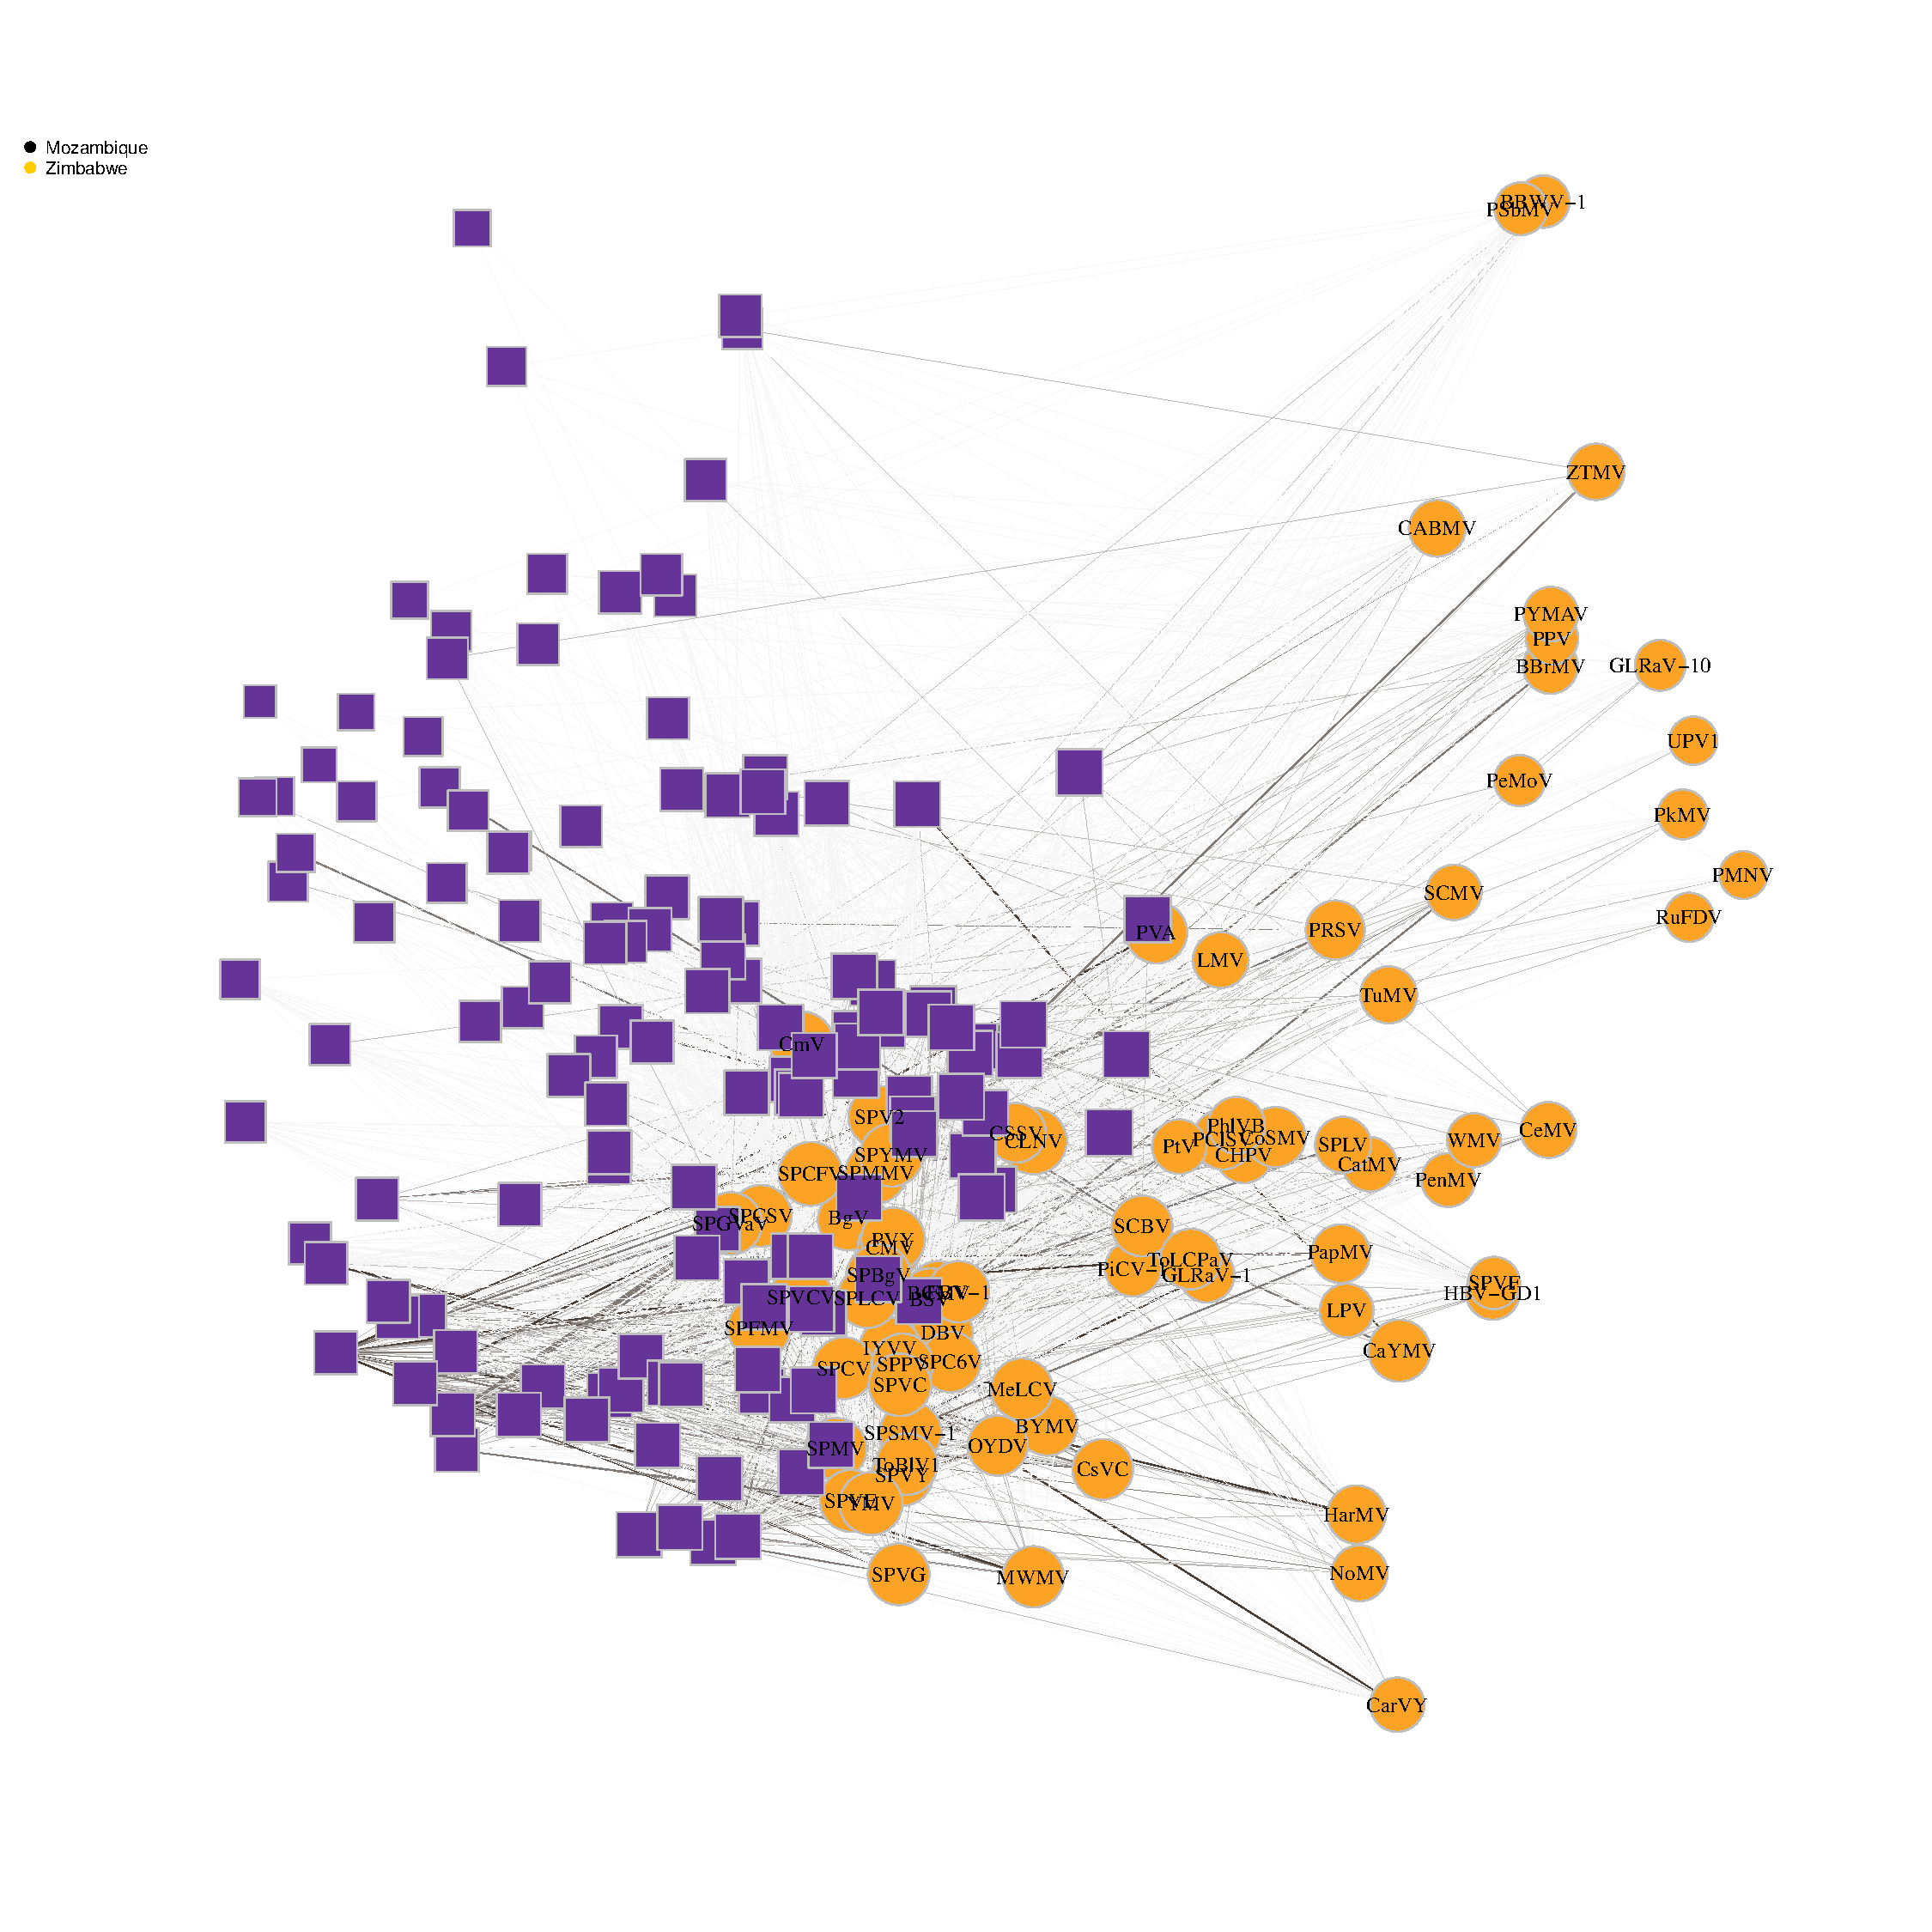
\includegraphics[width=0.85\textwidth]{../results/k-cluster5/5-kcluster_bipartitenetwork-kk_Feb28.pdf
} % Include the image placeholder.png
\caption{Bipartite network Sub-Saharan Africa sweetpotato virome region 1, Kimura-Kawai layout}
\end{center}
\end{figure}

\subsection{Region 6}

\begin{figure}[h!]
\begin{center}
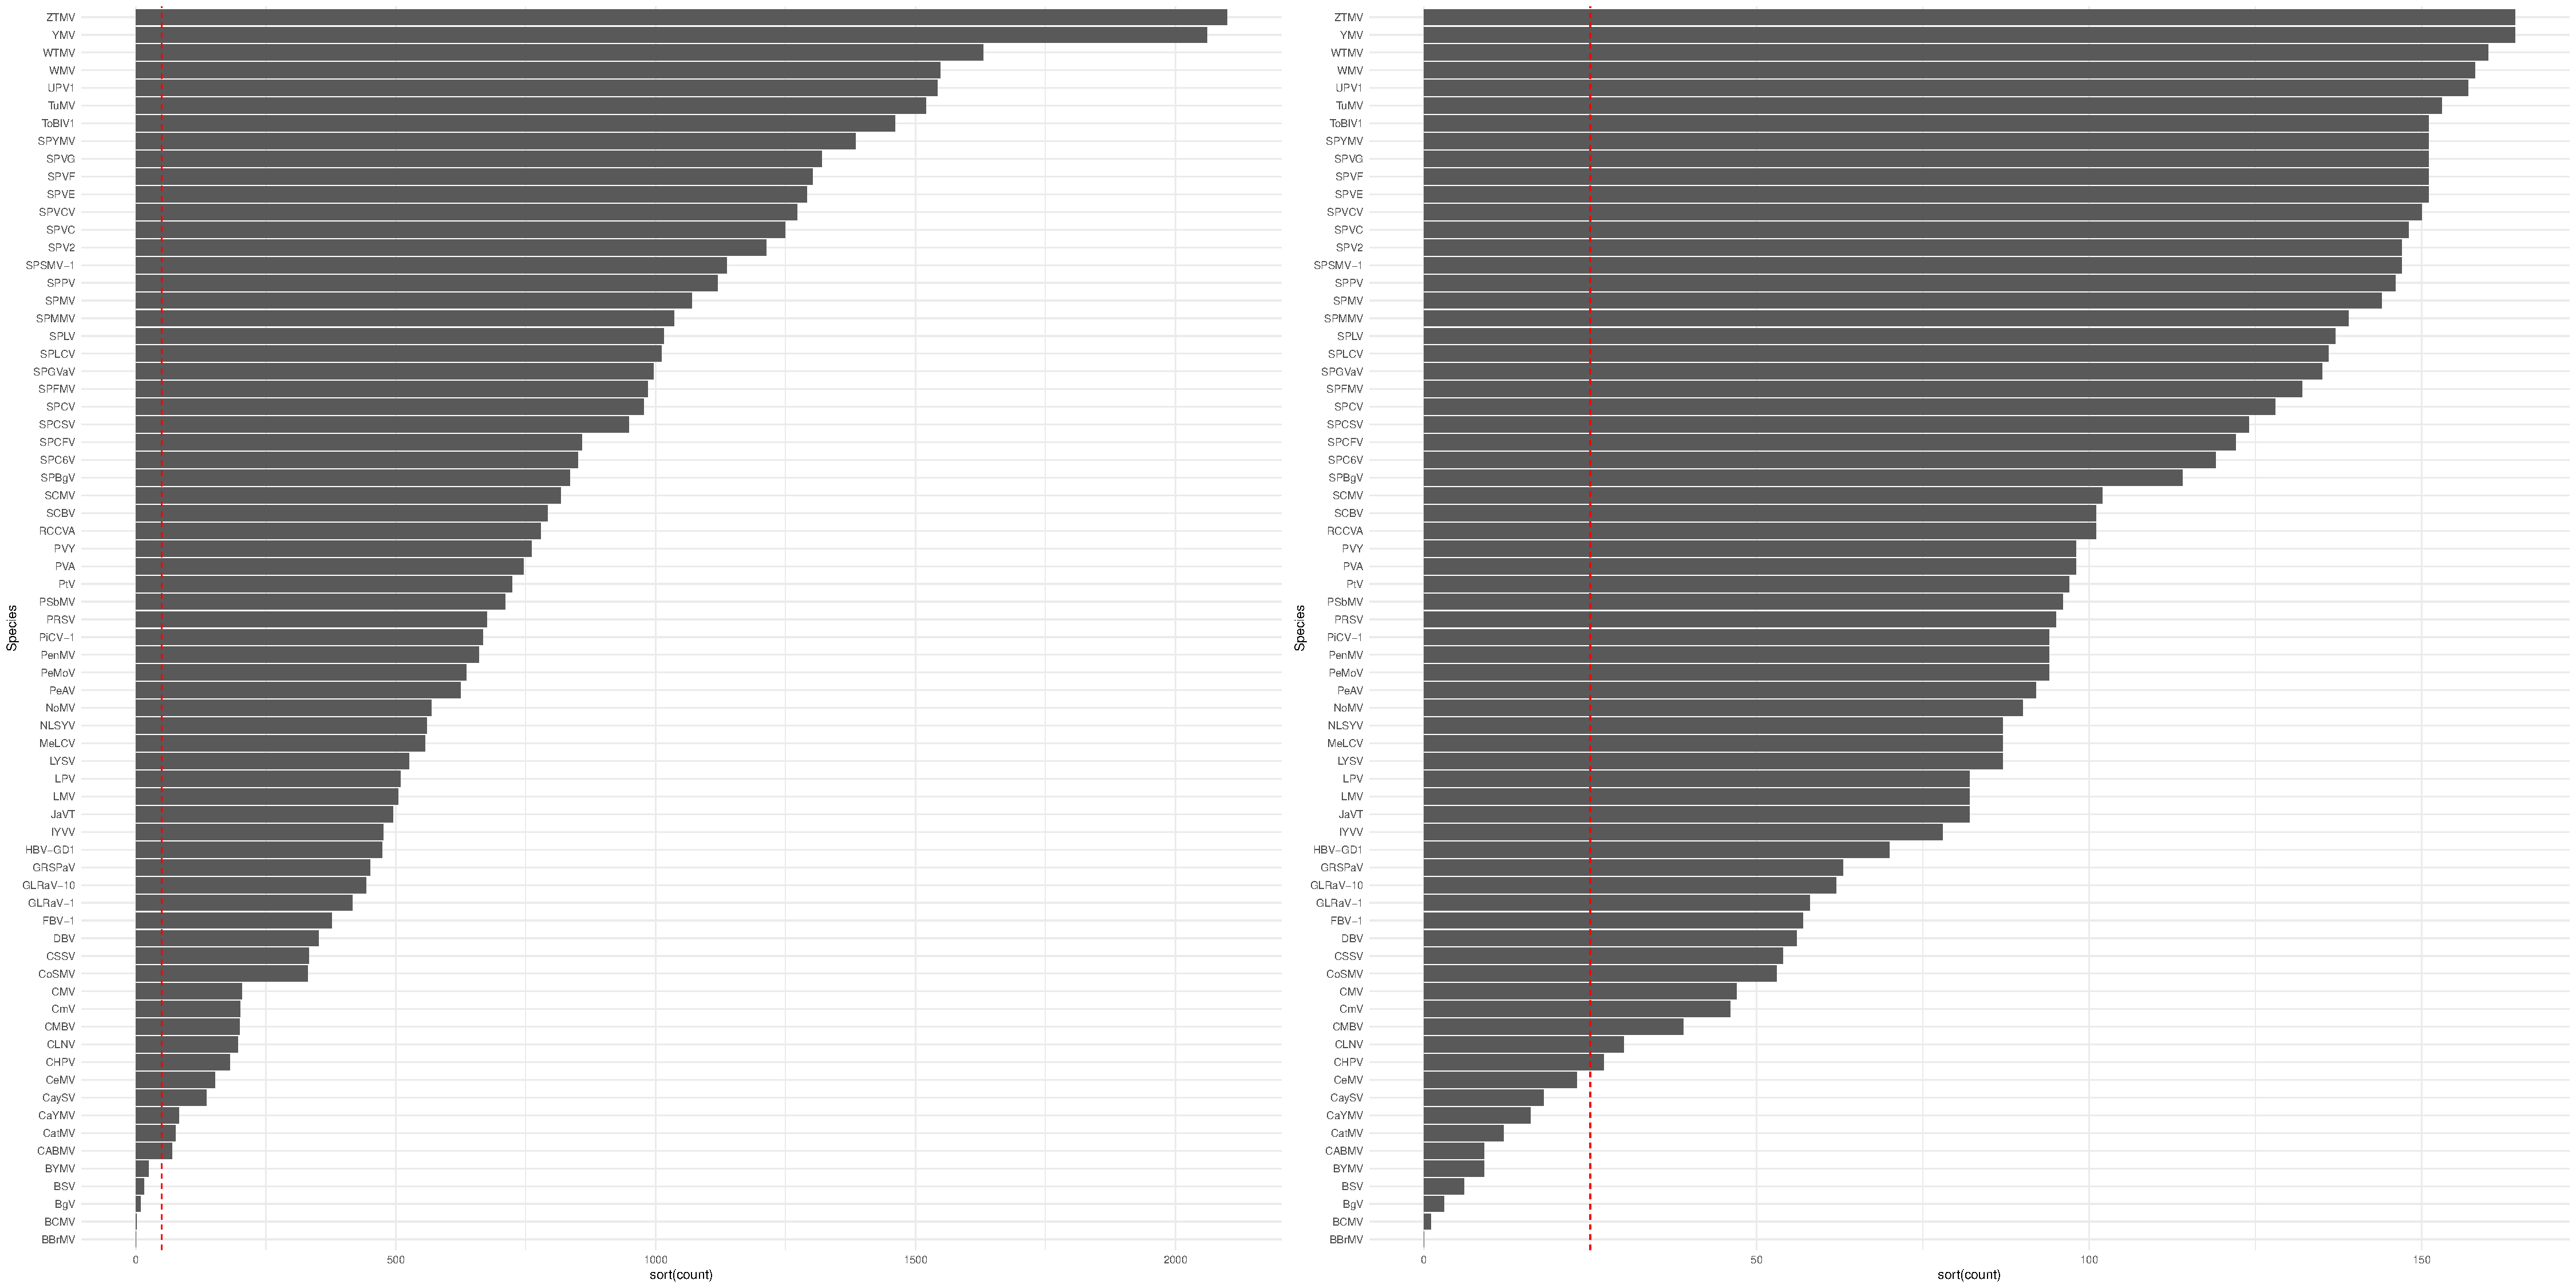
\includegraphics[width=0.95\textwidth]{../results/k-cluster6/6-kcluster_incidence_w+bFeb28.pdf
} % Include the image placeholder.png
\caption{Incidence distribution Sub-Saharan Africa sweetpotato virome region 1.}
\end{center}
\end{figure}


\begin{figure}[h!]
\begin{center}
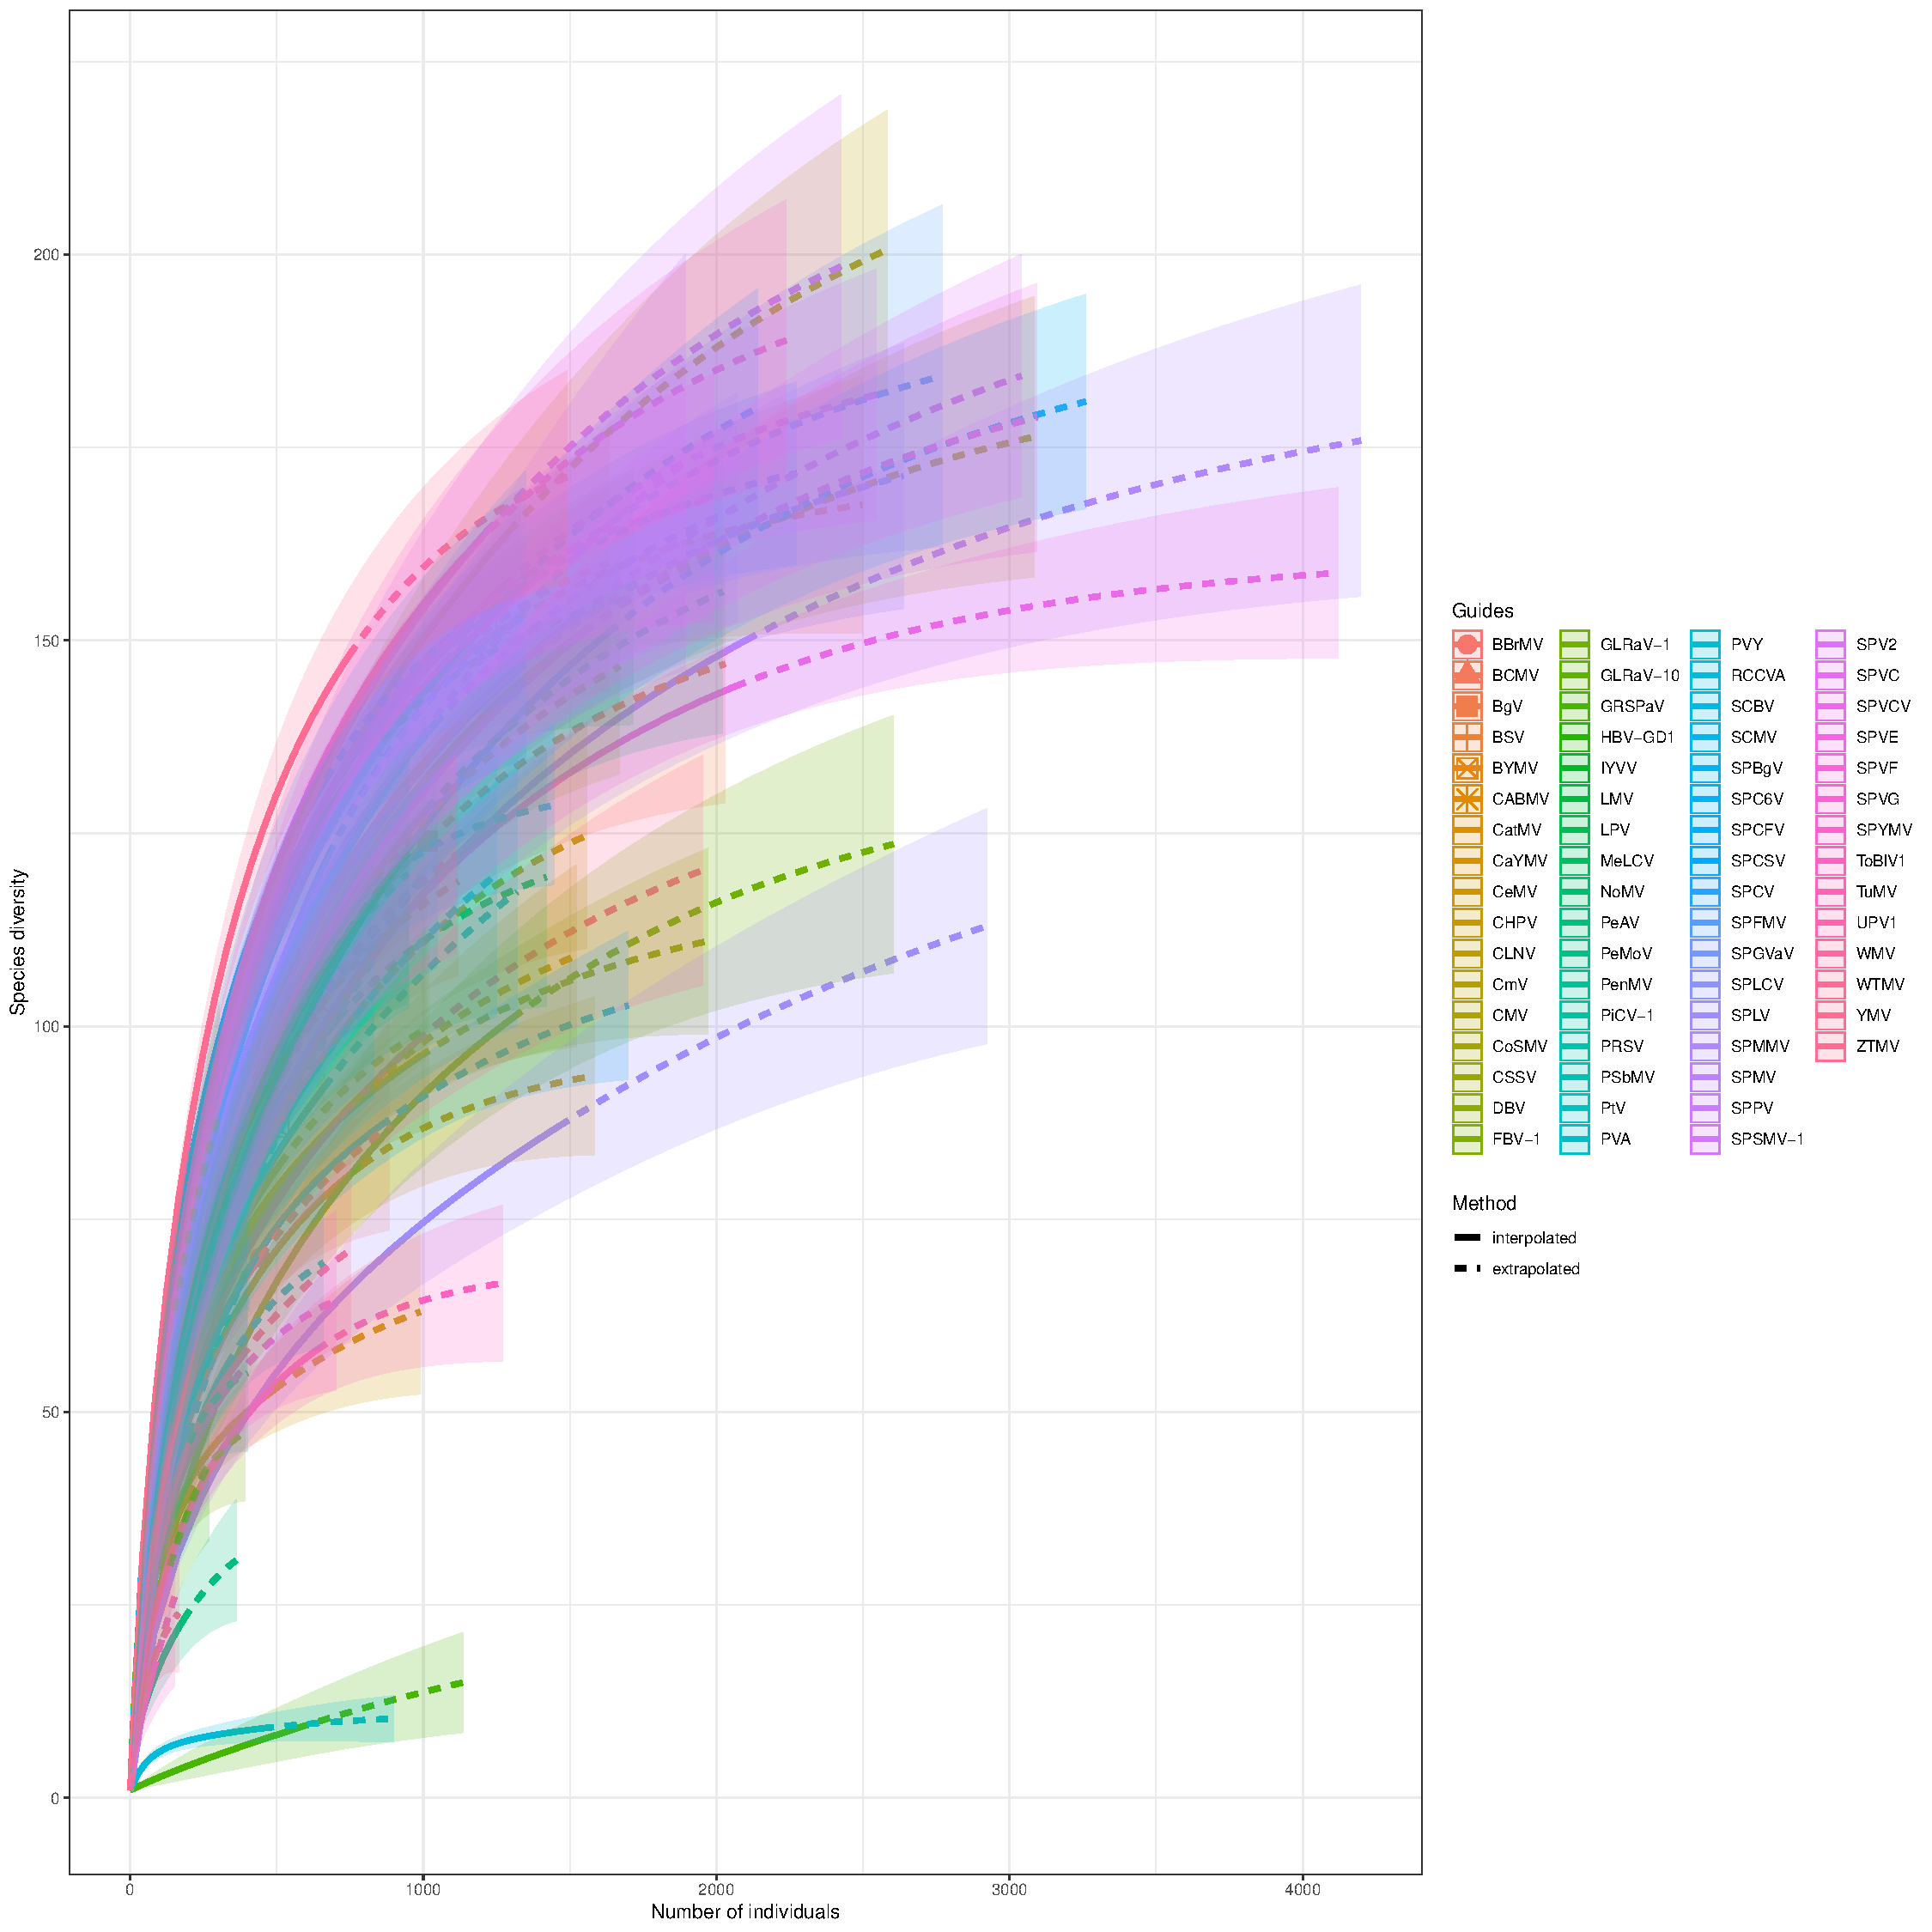
\includegraphics[width=0.75\textwidth]{../results/k-cluster6/6-kcluster_rarefaction-iNEXT_Feb28.pdf
} % Include the image placeholder.png
\caption{Rarefaction of Sub-Saharan Africa sweetpotato virome region 1.}
\end{center}
\end{figure}


\begin{figure}[h!]
\begin{center}
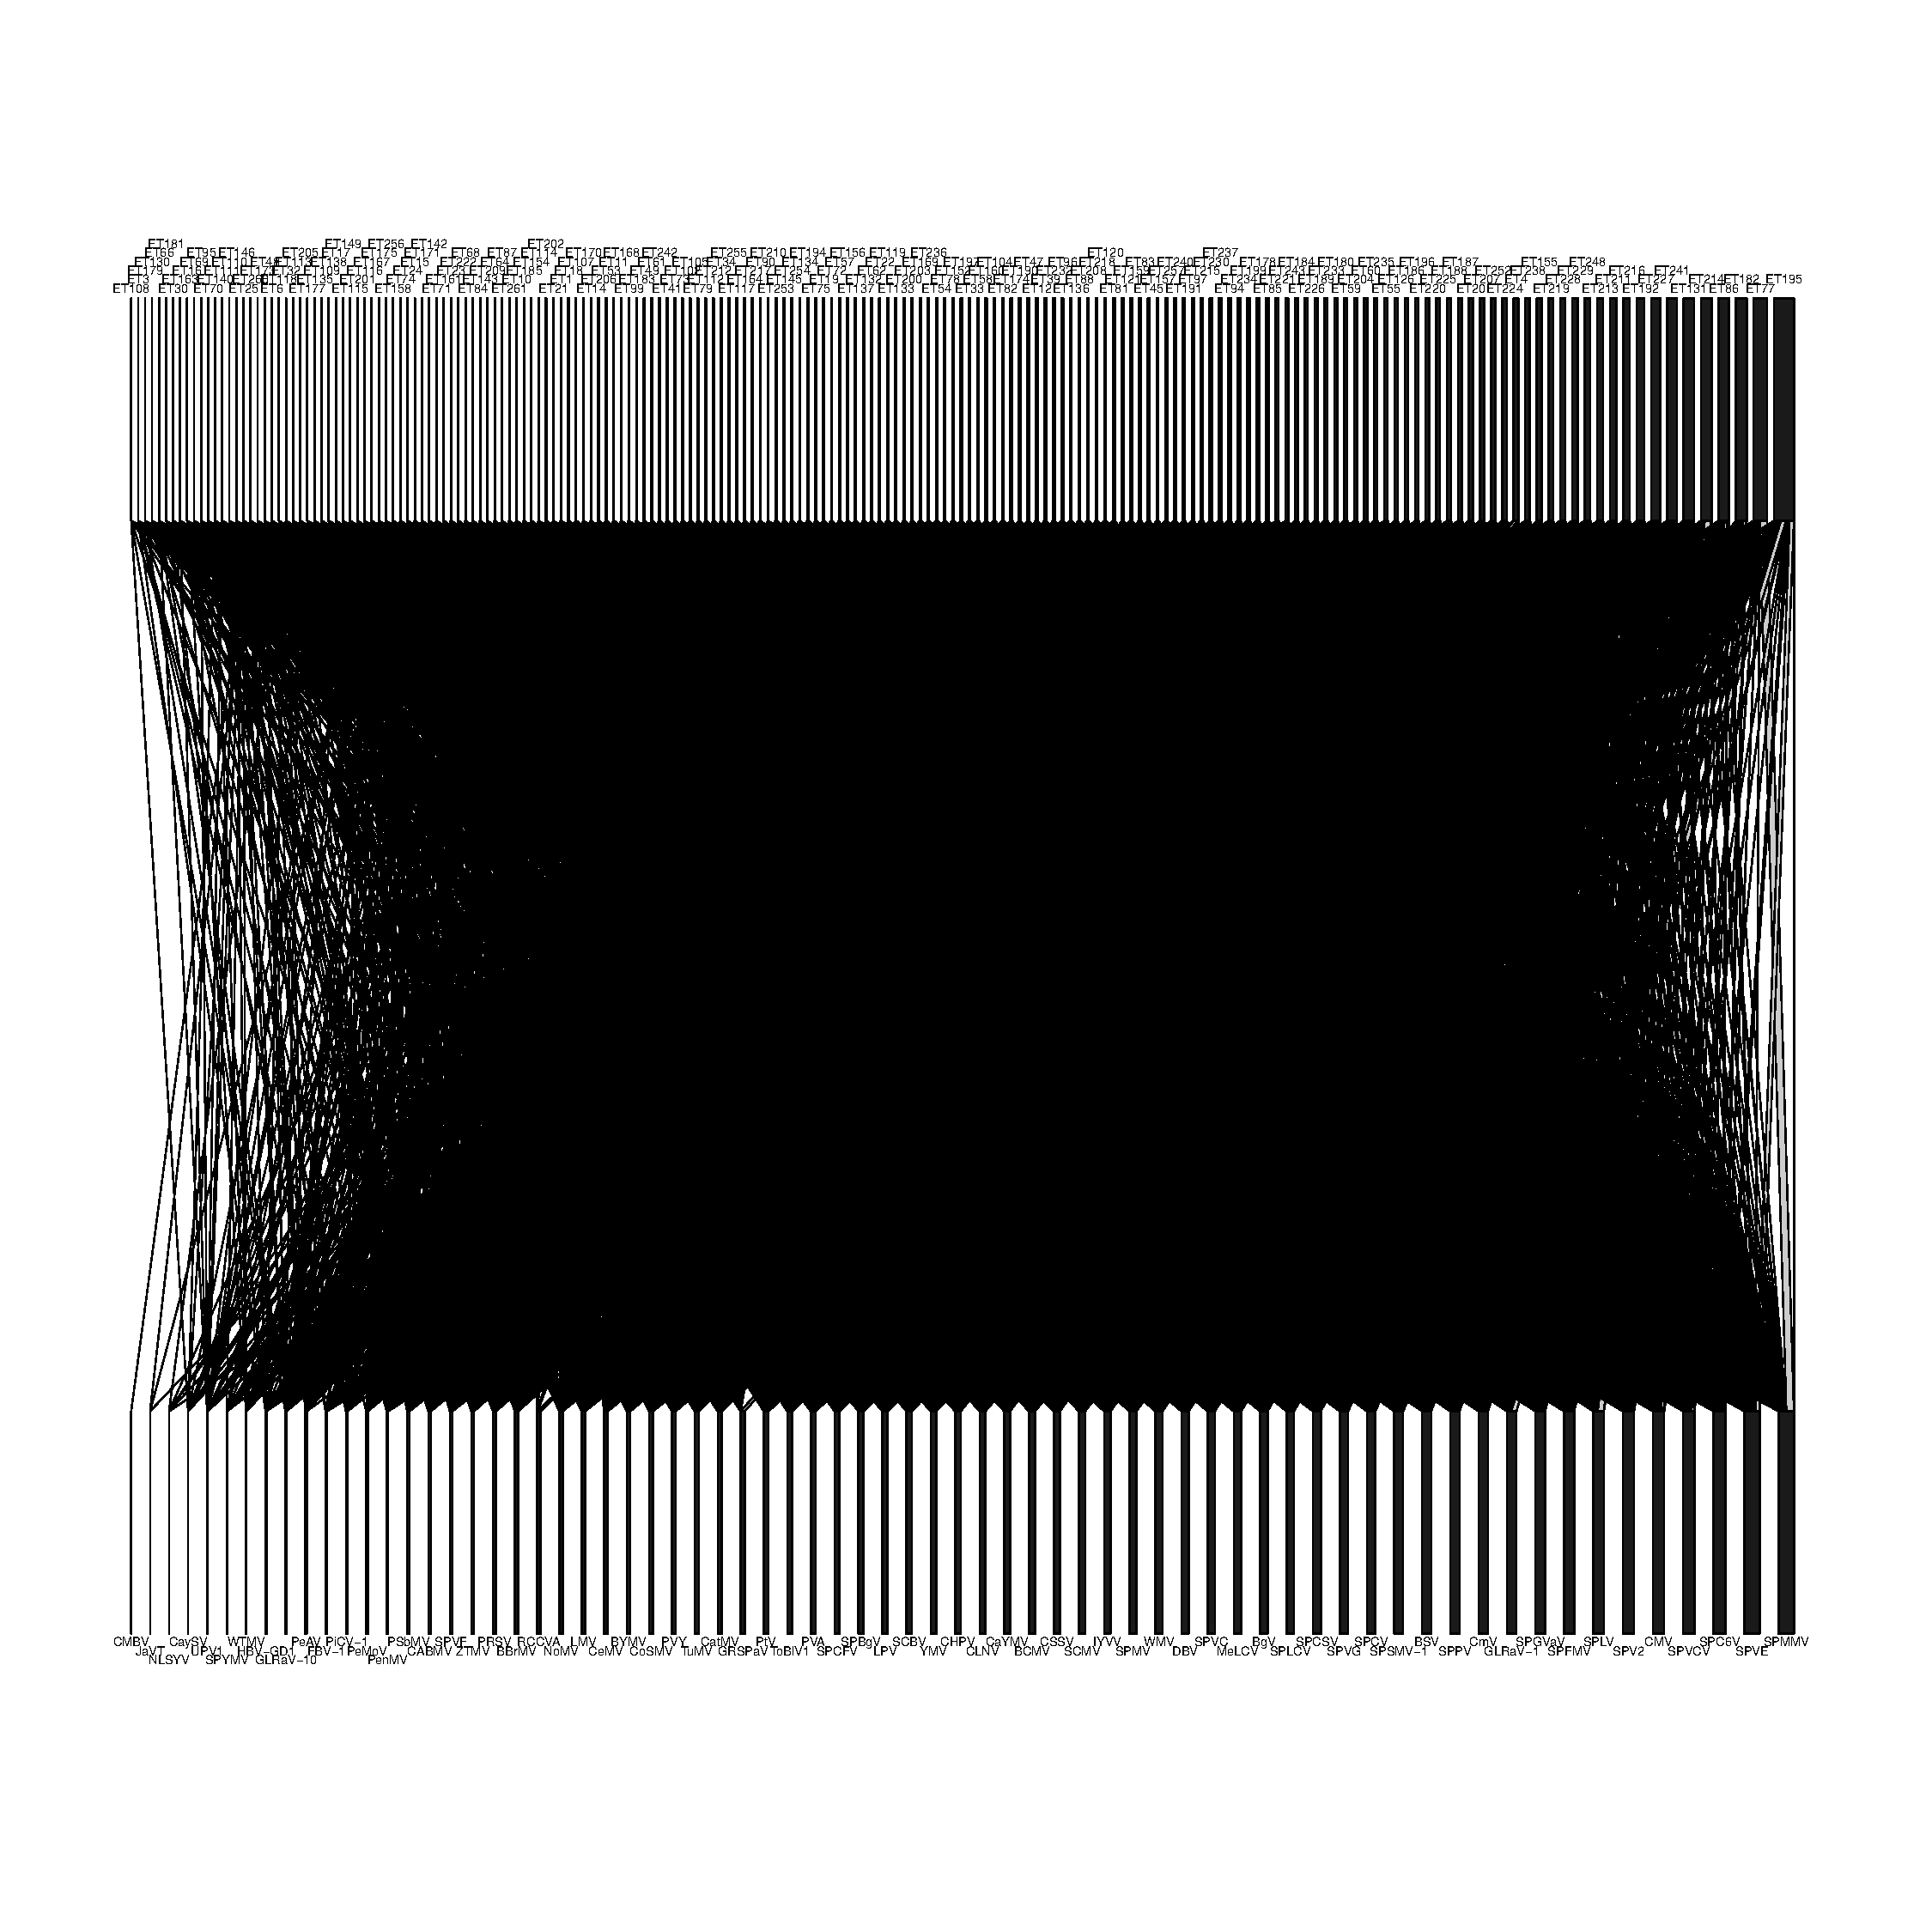
\includegraphics[width=0.75\textwidth]{../results/k-cluster6/6-kcluster_bipartitenetwork_Feb28.pdf
} % Include the image placeholder.png
\caption{Bipartite network Sub-Saharan Africa sweetpotato virome region 1.}
\end{center}
\end{figure}



\begin{figure}[h!]
\begin{center}
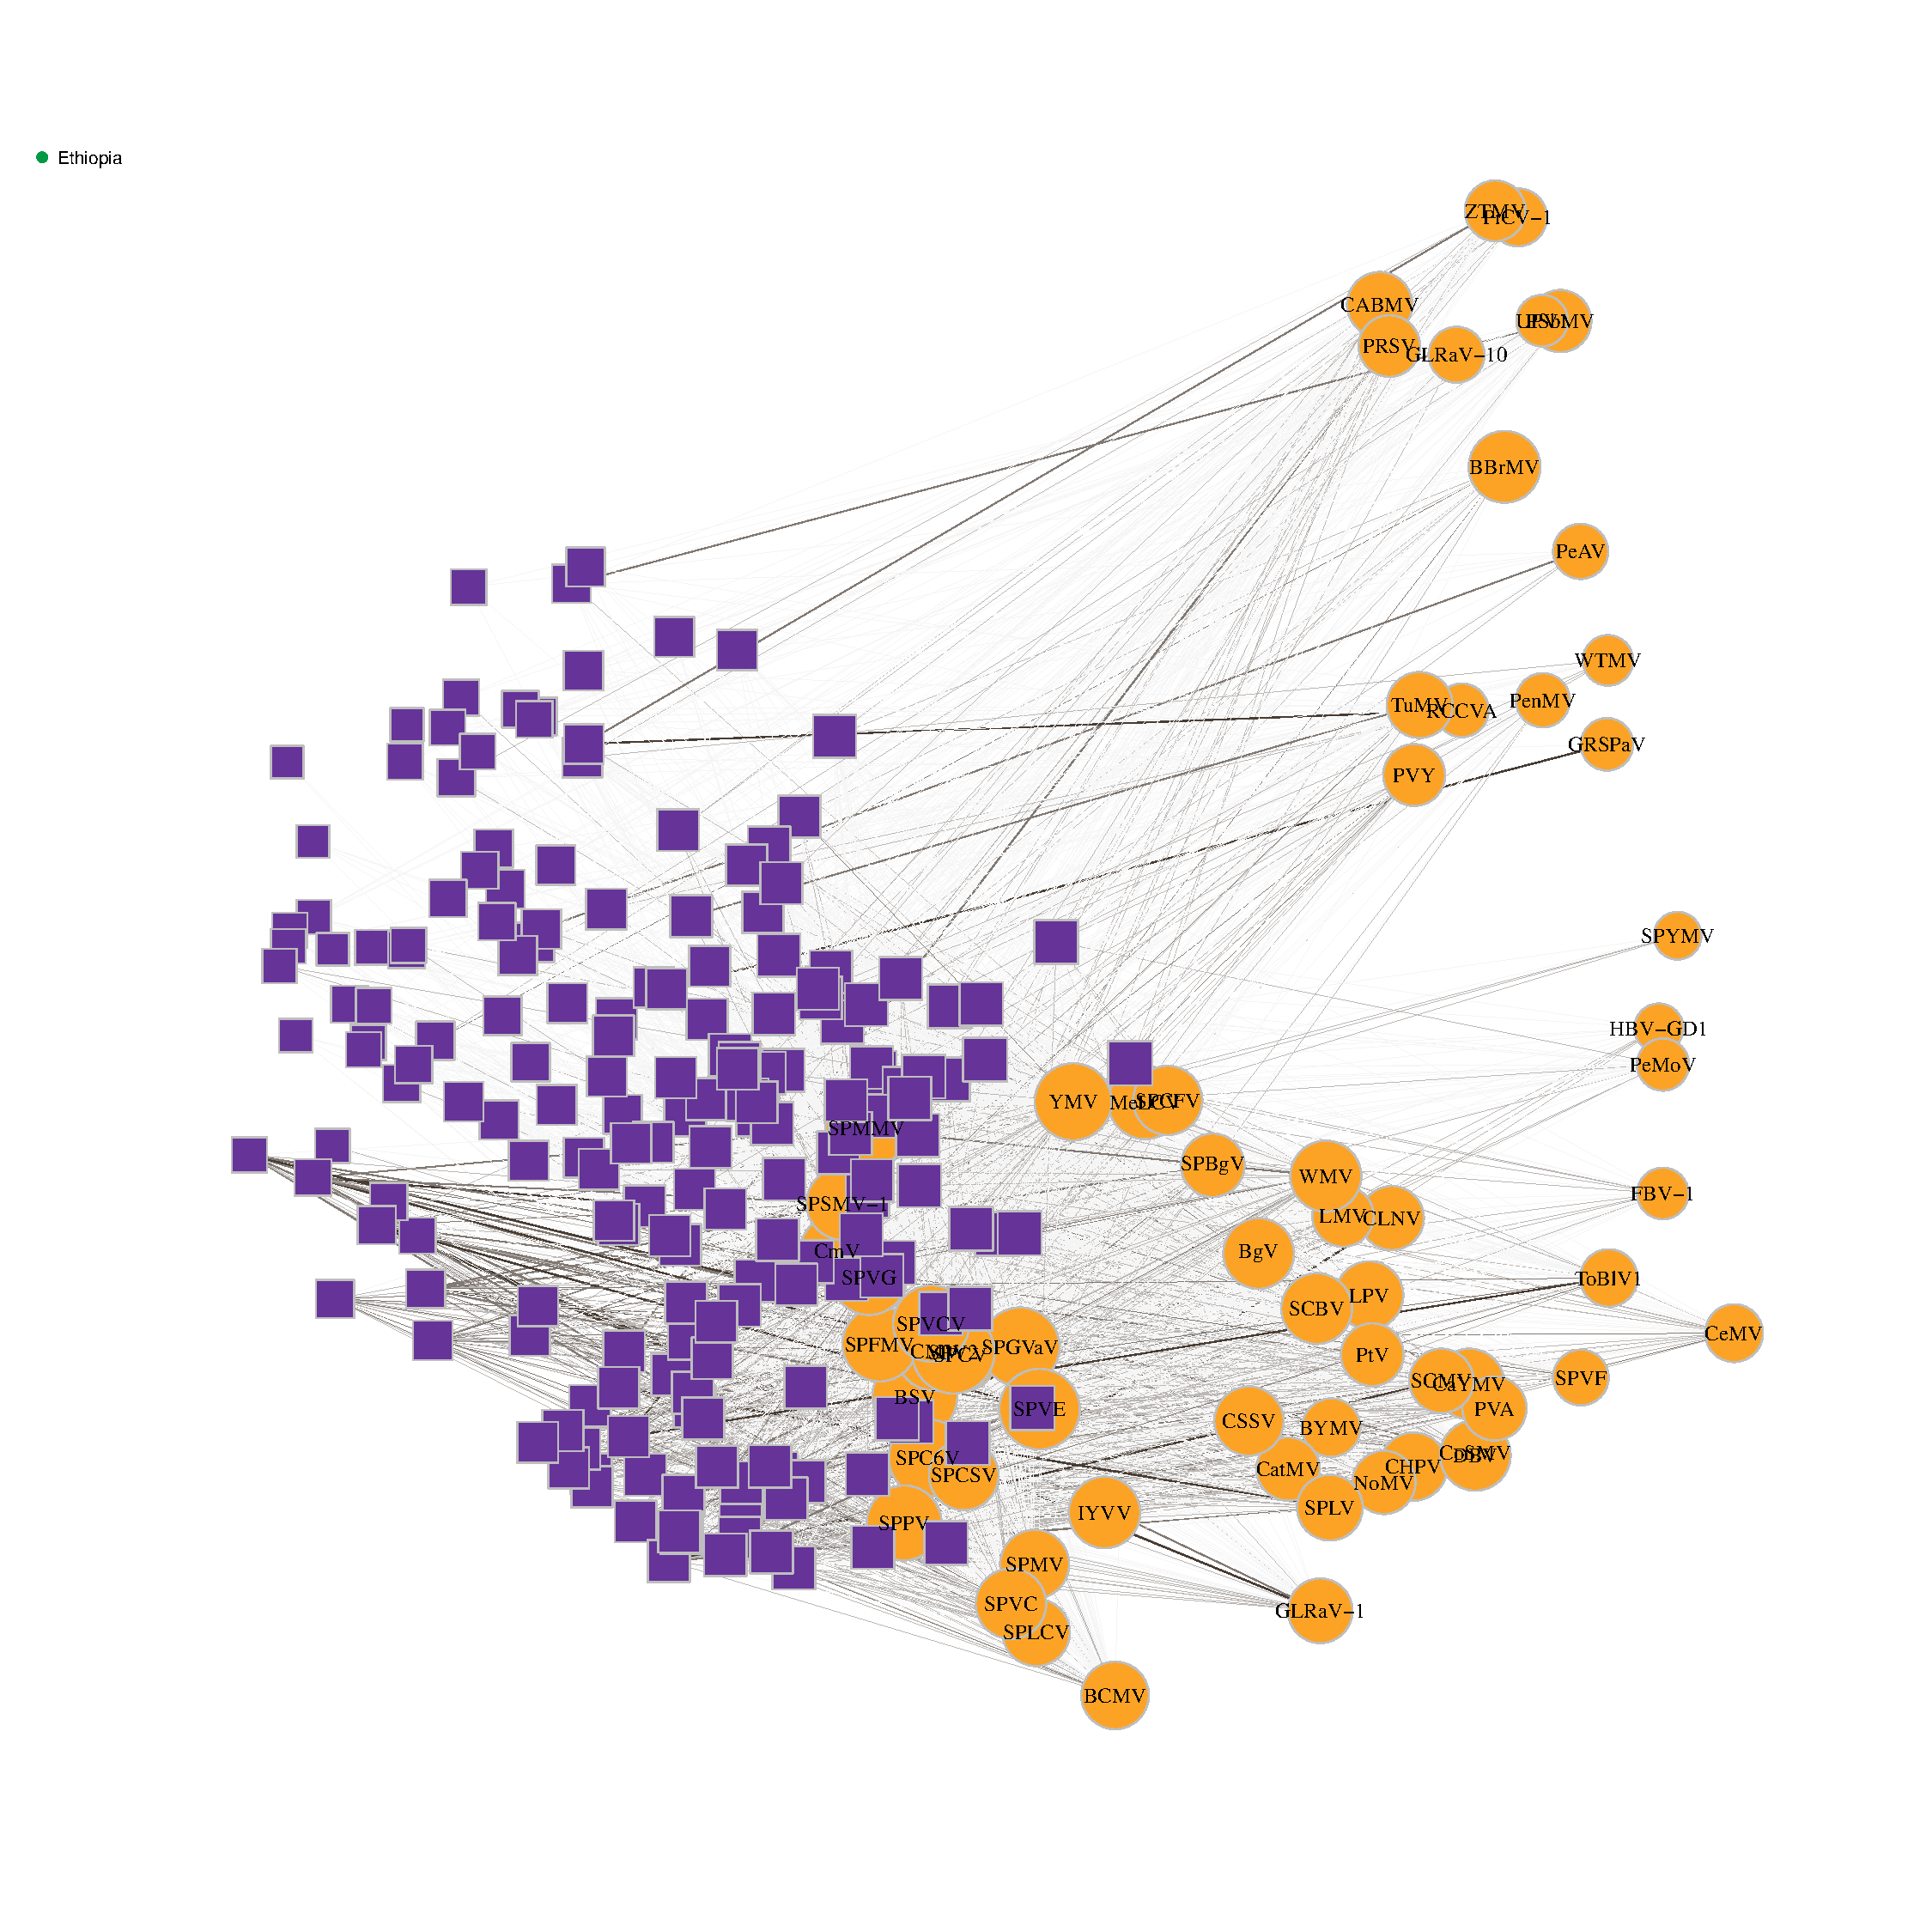
\includegraphics[width=0.85\textwidth]{../results/k-cluster6/6-kcluster_bipartitenetwork-kk_Feb28.pdf
} % Include the image placeholder.png
\caption{Bipartite network Sub-Saharan Africa sweetpotato virome region 1, Kimura-Kawai layout}
\end{center}
\end{figure}

\subsection{Region 7}

\begin{figure}[h!]
\begin{center}
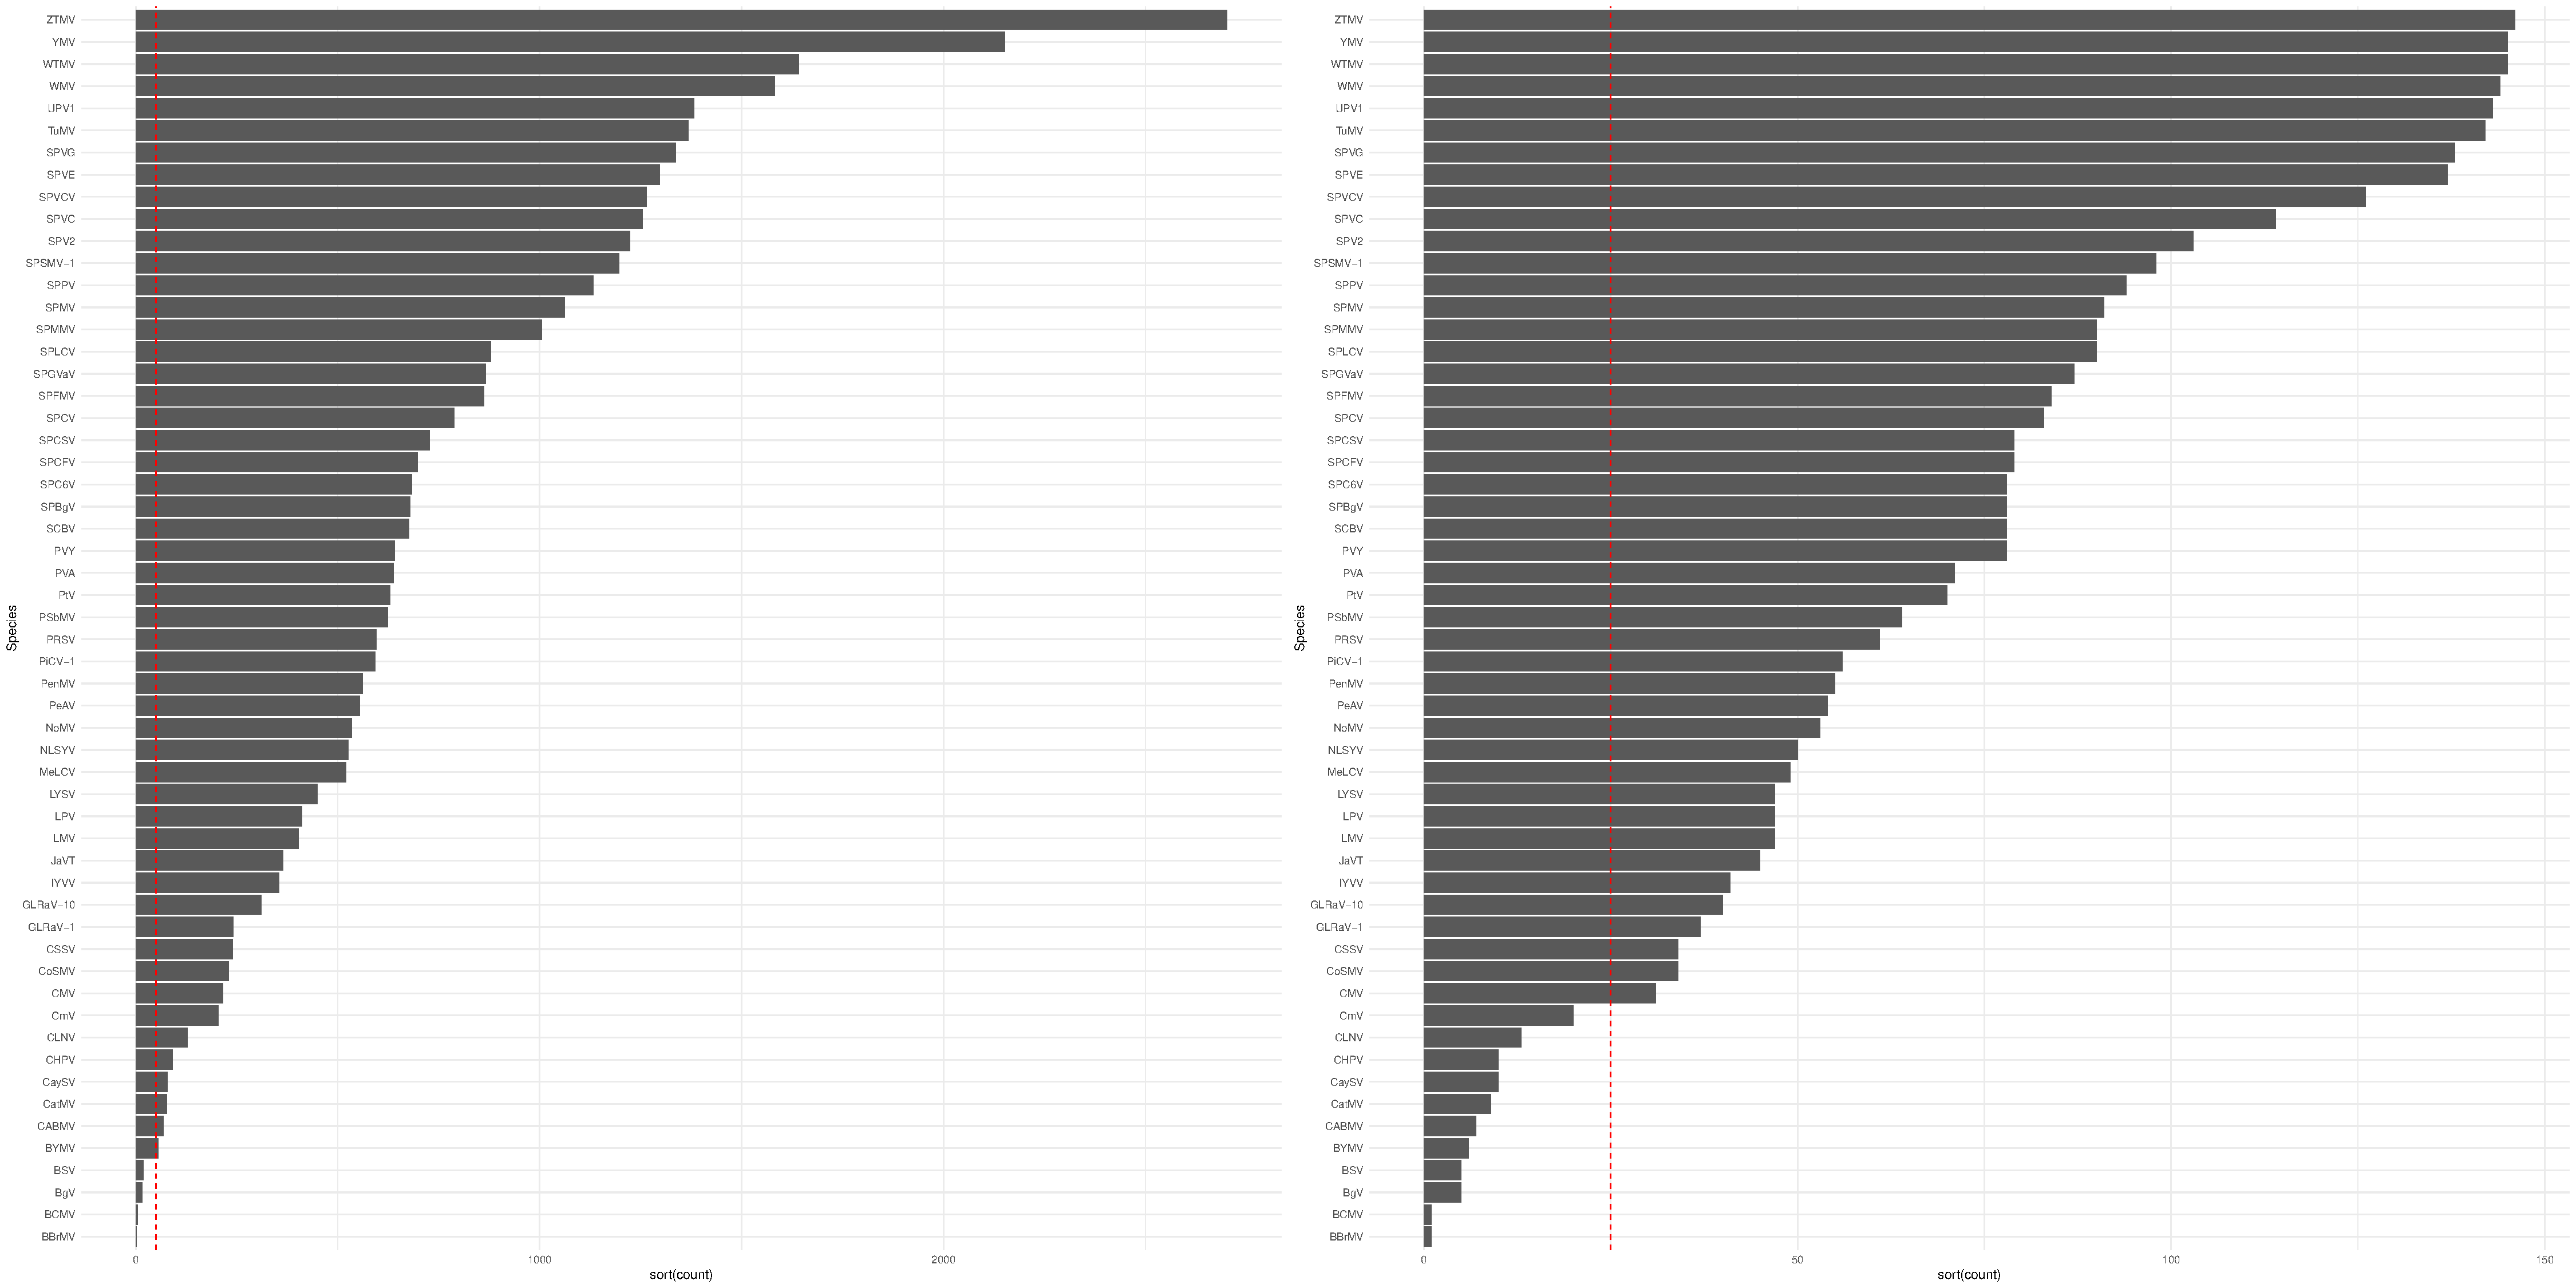
\includegraphics[width=0.95\textwidth]{../results/k-cluster7/7-kcluster_incidence_w+bFeb28.pdf
} % Include the image placeholder.png
\caption{Incidence distribution Sub-Saharan Africa sweetpotato virome region 1.}
\end{center}
\end{figure}


\begin{figure}[h!]
\begin{center}
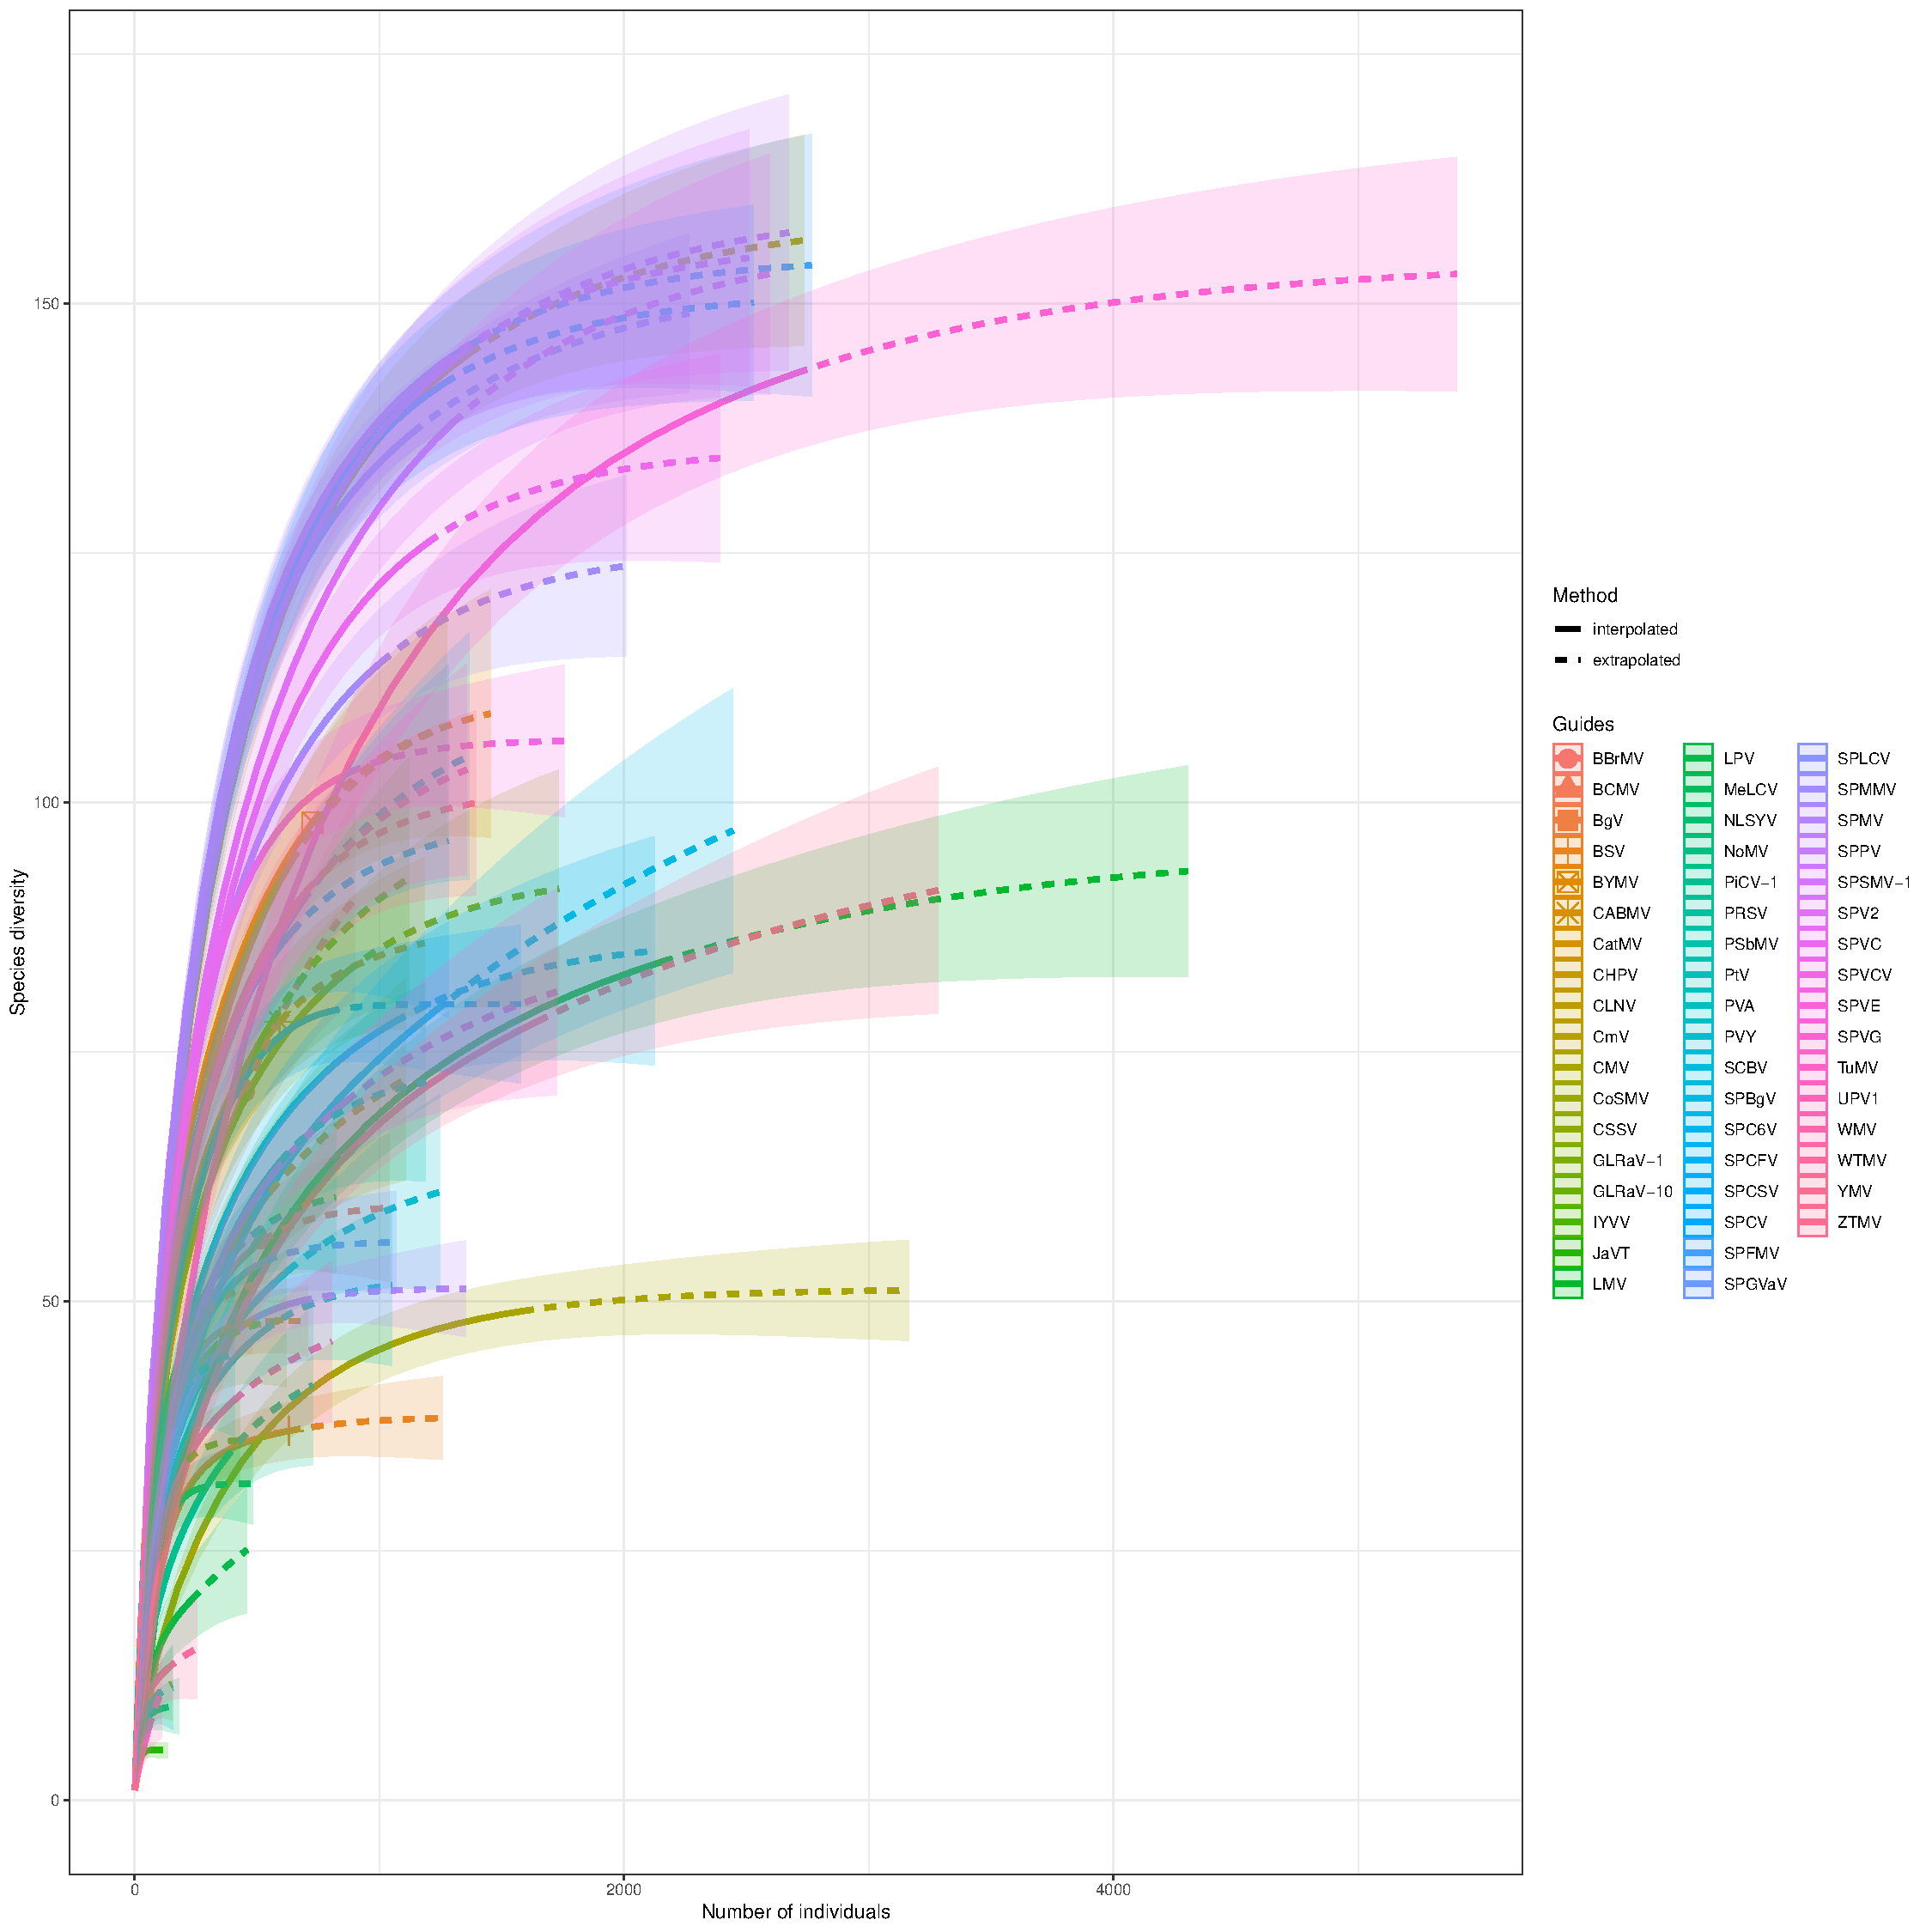
\includegraphics[width=0.75\textwidth]{../results/k-cluster7/7-kcluster_rarefaction-iNEXT_Feb28.pdf
} % Include the image placeholder.png
\caption{Rarefaction of Sub-Saharan Africa sweetpotato virome region 1.}
\end{center}
\end{figure}


\begin{figure}[h!]
\begin{center}
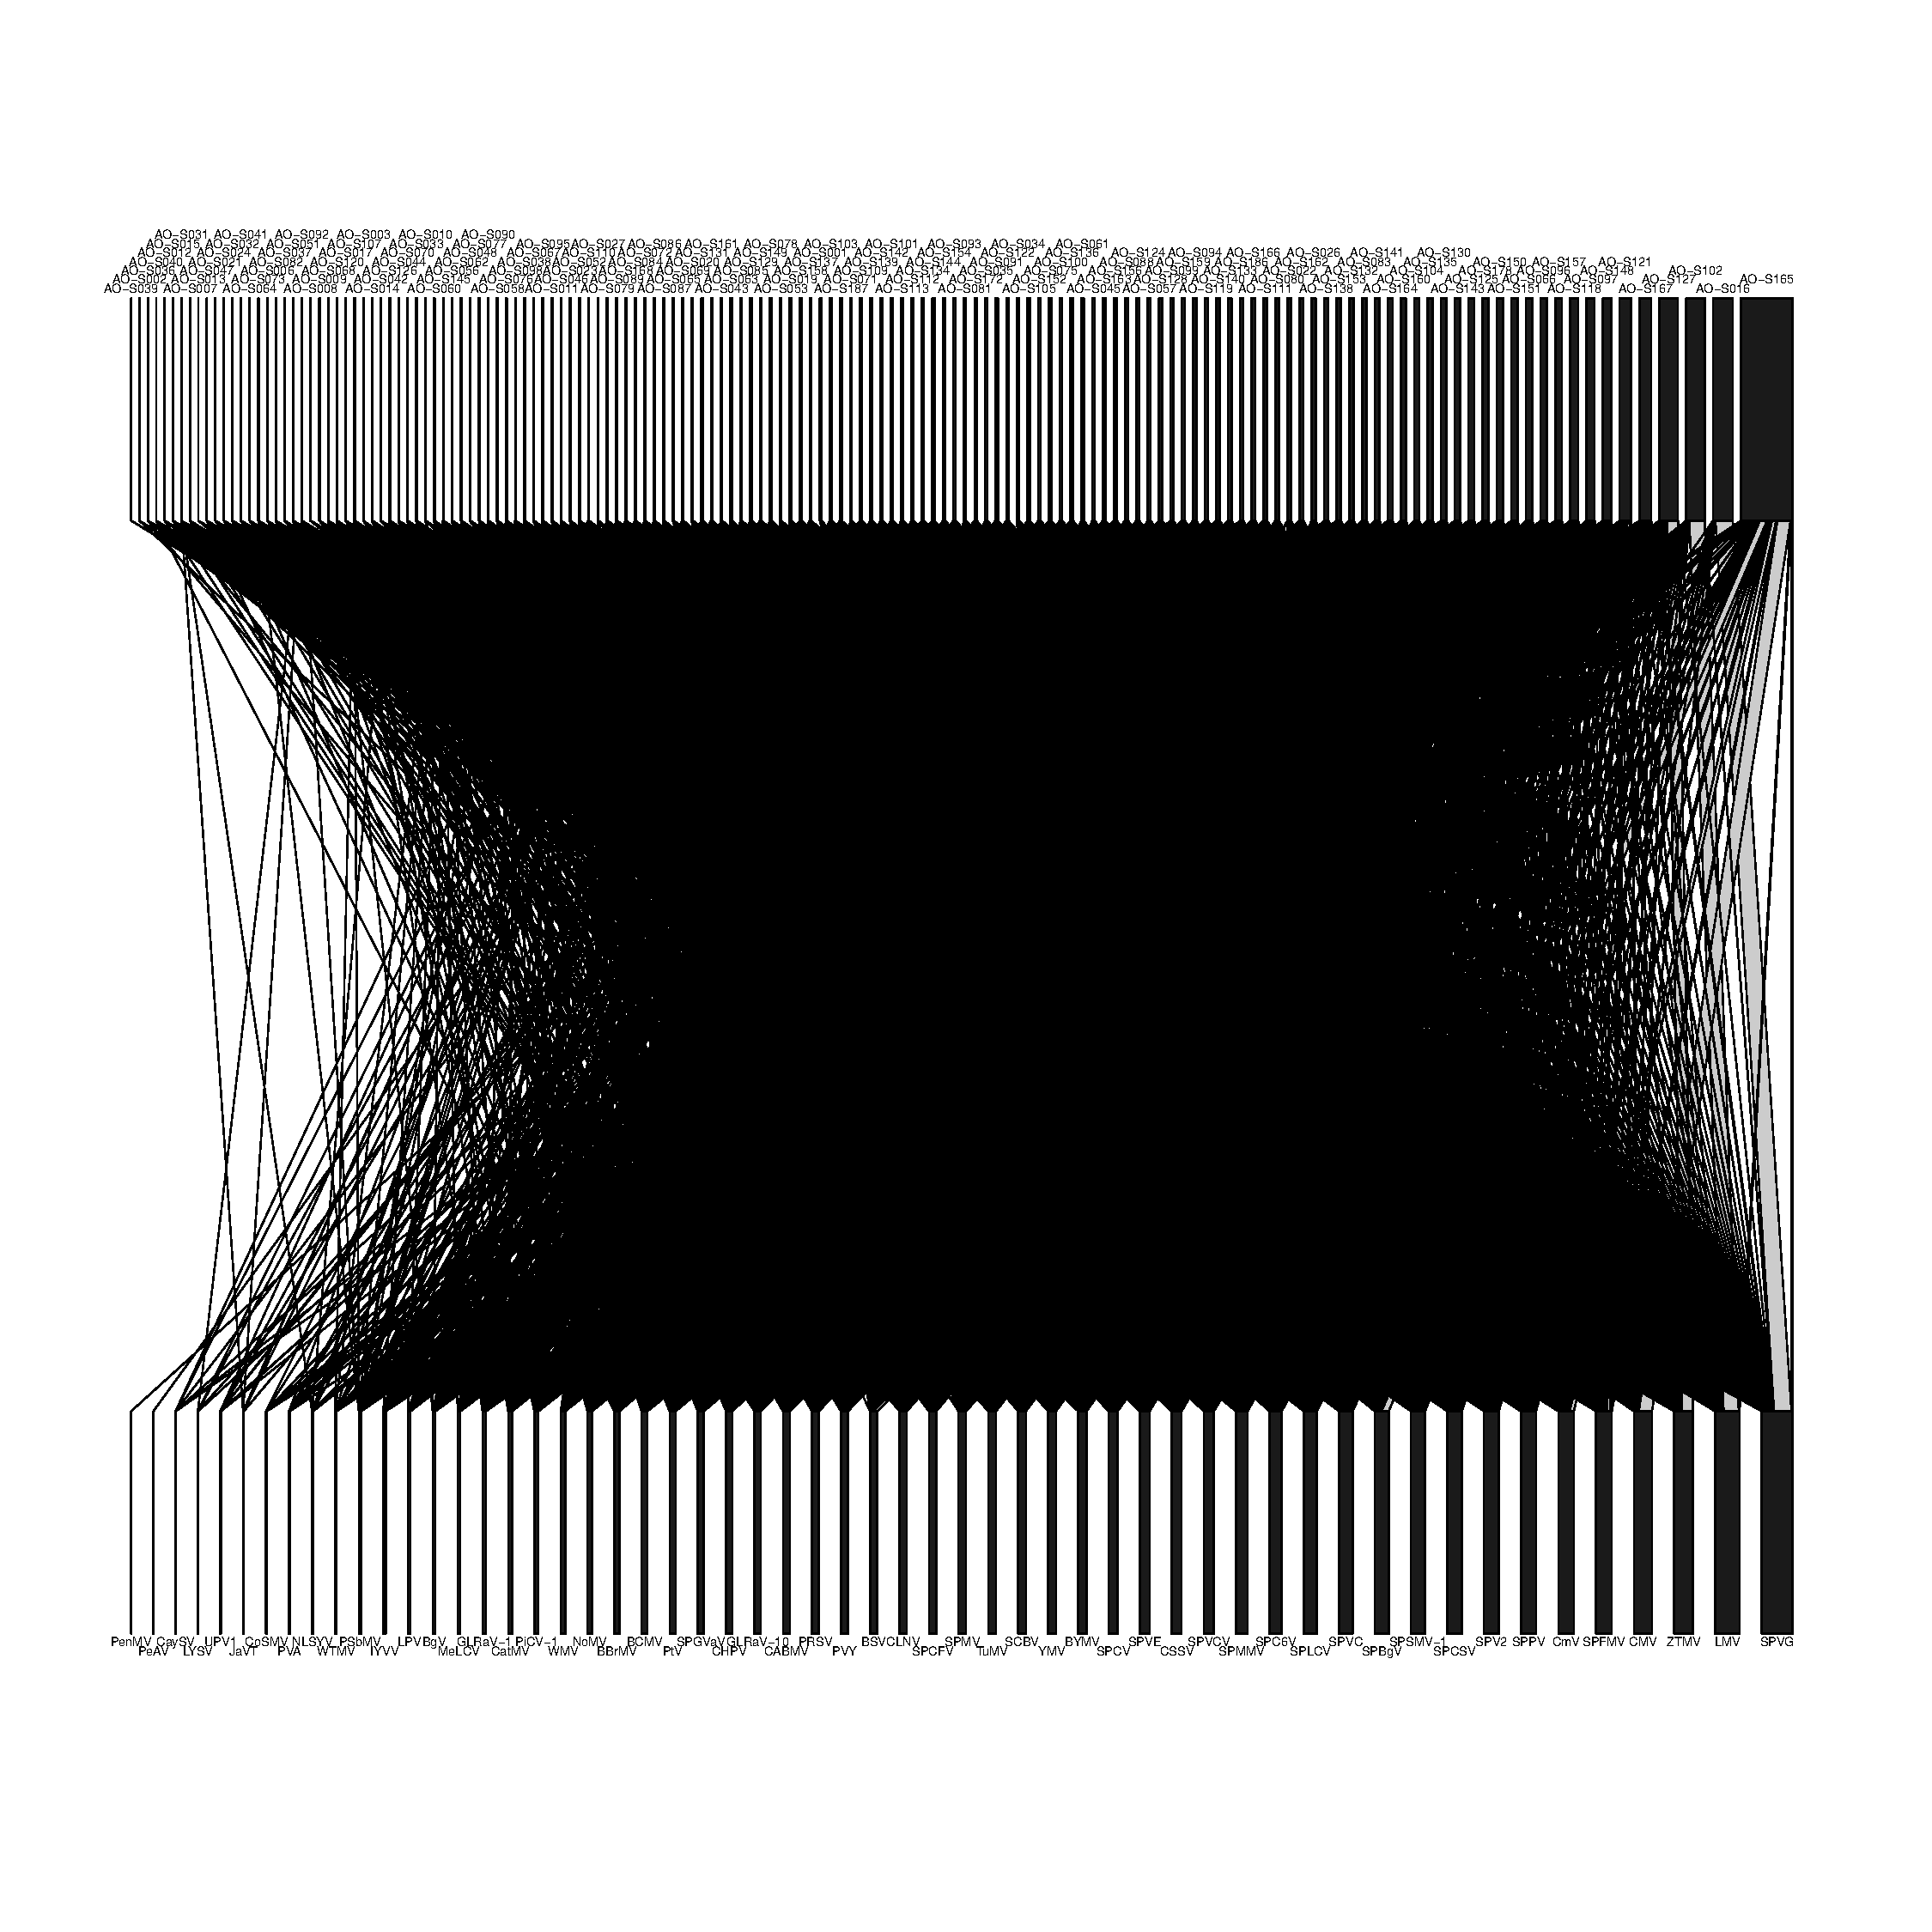
\includegraphics[width=0.75\textwidth]{../results/k-cluster7/7-kcluster_bipartitenetwork_Feb28.pdf
} % Include the image placeholder.png
\caption{Bipartite network Sub-Saharan Africa sweetpotato virome region 1.}
\end{center}
\end{figure}



\begin{figure}[h!]
\begin{center}
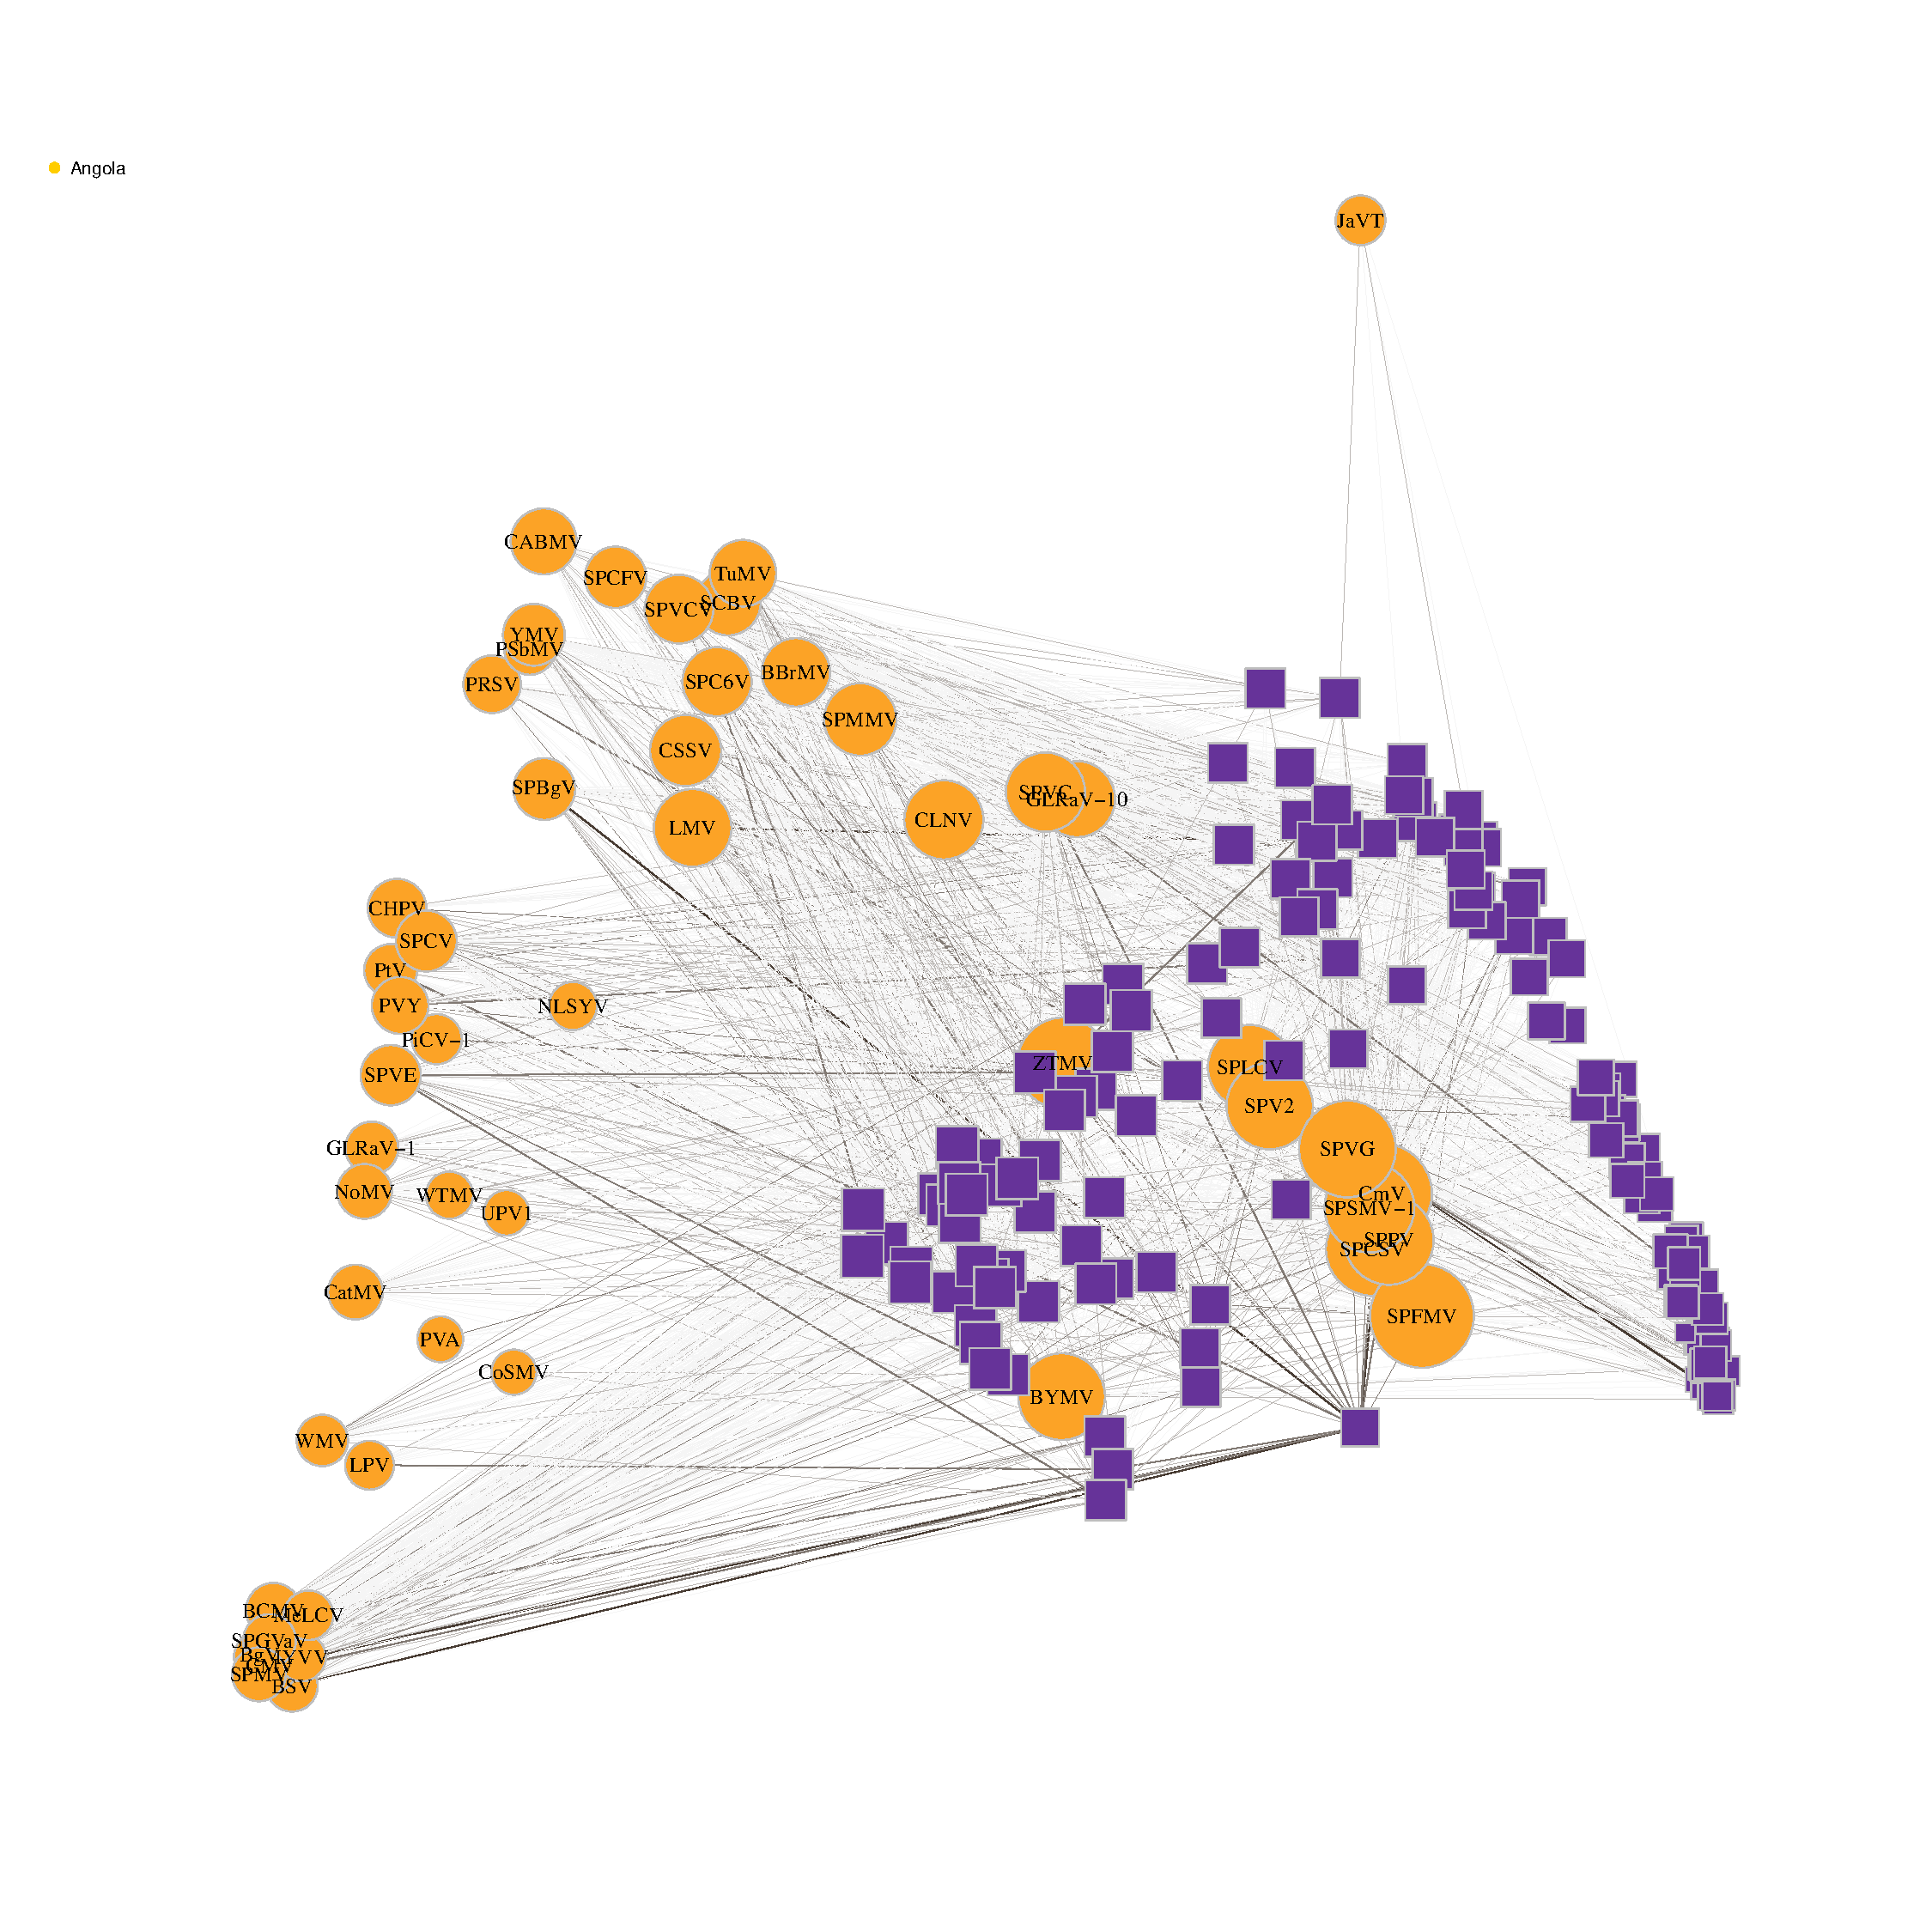
\includegraphics[width=0.85\textwidth]{../results/k-cluster7/7-kcluster_bipartitenetwork-kk_Feb28.pdf
} % Include the image placeholder.png
\caption{Bipartite network Sub-Saharan Africa sweetpotato virome region 1, Kimura-Kawai layout}
\end{center}
\end{figure}

%----------------------------------------------------------------------------------------
%	SECTION 3
%----------------------------------------------------------------------------------------

\section{Networks metrics}

\begin{tabular}{ll}
Mass of magnesium metal & = \SI{8.59}{\gram} - \SI{7.28}{\gram}\\
& = \SI{1.31}{\gram}\\
Mass of magnesium oxide & = \SI{9.46}{\gram} - \SI{7.28}{\gram}\\
& = \SI{2.18}{\gram}\\
Mass of oxygen & = \SI{2.18}{\gram} - \SI{1.31}{\gram}\\
& = \SI{0.87}{\gram}
\end{tabular}

Because of this reaction, the required ratio is the atomic weight of magnesium: \SI{16.00}{\gram} of oxygen as experimental mass of Mg: experimental mass of oxygen or $\frac{x}{1.31}=\frac{16}{0.87}$ from which, $M_{\ce{Mg}} = 16.00 \times \frac{1.31}{0.87} = 24.1 = \SI{24}{\gram\per\mole}$ (to two significant figures).

%----------------------------------------------------------------------------------------
%	SECTION 4
%----------------------------------------------------------------------------------------

\section{Results and Conclusions}

The atomic weight of magnesium is concluded to be \SI{24}{\gram\per\mol}, as determined by the stoichiometry of its chemical combination with oxygen. This result is in agreement with the accepted value.

\begin{figure}[h]
\begin{center}

\includegraphics[width=0.65\textwidth]{placeholder} % Include the image placeholder.png
\caption{Figure caption.}
\end{center}
\end{figure}

%----------------------------------------------------------------------------------------
%	SECTION 5
%----------------------------------------------------------------------------------------

\section{Discussion of Experimental Uncertainty}

The accepted value (periodic table) is \SI{24.3}{\gram\per\mole} \cite{Smith:2012qr}. The percentage discrepancy between the accepted value and the result obtained here is 1.3\%. Because only a single measurement was made, it is not possible to calculate an estimated standard deviation.

The most obvious source of experimental uncertainty is the limited precision of the balance. Other potential sources of experimental uncertainty are: the reaction might not be complete; if not enough time was allowed for total oxidation, less than complete oxidation of the magnesium might have, in part, reacted with nitrogen in the air (incorrect reaction); the magnesium oxide might have absorbed water from the air, and thus weigh ``too much." Because the result obtained is close to the accepted value it is possible that some of these experimental uncertainties have fortuitously cancelled one another.

%----------------------------------------------------------------------------------------
%	SECTION 6
%----------------------------------------------------------------------------------------

\section{Answers to Definitions}

\begin{enumerate}
\begin{item}
The \emph{atomic weight of an element} is the relative weight of one of its atoms compared to C-12 with a weight of 12.0000000$\ldots$, hydrogen with a weight of 1.008, to oxygen with a weight of 16.00. Atomic weight is also the average weight of all the atoms of that element as they occur in nature.
\end{item}
\begin{item}
The \emph{units of atomic weight} are two-fold, with an identical numerical value. They are g/mole of atoms (or just g/mol) or amu/atom.
\end{item}
\begin{item}
\emph{Percentage discrepancy} between an accepted (literature) value and an experimental value is
\begin{equation*}
\frac{\mathrm{experimental\;result} - \mathrm{accepted\;result}}{\mathrm{accepted\;result}}
\end{equation*}
\end{item}
\end{enumerate}

%----------------------------------------------------------------------------------------
%	BIBLIOGRAPHY
%----------------------------------------------------------------------------------------

\bibliographystyle{apalike}

\bibliography{sample}

%----------------------------------------------------------------------------------------


\end{document}